% !TeX spellcheck = fr_FR
%%%%%%%%%%%%%%%%%%%%%%%%%%%%%%%%%%%%%%%%%
% Created by Natanael Braga
% 06.03.2017
% Changelog: -v1: customized title page, added TOC, added headers and footers
%----------------------------------------------------------------------
% PACKAGES AND OTHER DOCUMENT CONFIGURATIONS
%----------------------------------------------------------------------
\documentclass[a4paper, 12pt]{article}
\usepackage[francais]{babel}
\usepackage[utf8]{inputenc}
\usepackage[T1]{fontenc}
\usepackage{lastpage}
\usepackage{listings}
\usepackage{textcomp}
\usepackage{float}
\usepackage{helvet}
\usepackage{amsmath}
\usepackage{pdfpages}
\usepackage{fancyhdr}
\usepackage{graphicx}
\usepackage{setspace}
\usepackage[colorinlistoftodos]{todonotes}
\usepackage[tmargin = 3.5cm, bmargin = 2cm, lmargin = 2.5cm, rmargin = 2cm, headheight=110pt]{geometry}
\usepackage{tocloft}
\renewcommand\cftsecdotsep{\cftdotsep}

\pagestyle{fancy}
\fancypagestyle{plain}

% customization for code listing
\lstset{
 backgroundcolor=\color{white},
 tabsize=4,
 language=java,
 basicstyle=\scriptsize,
 upquote=true,
 aboveskip={1.5\baselineskip},
 columns=fixed,
 showstringspaces=false,
 extendedchars=true,
 breaklines=true,
 frame=single,
 showtabs=false,
 showspaces=false,
 showstringspaces=false,
 identifierstyle=\ttfamily,
 keywordstyle=\color[RGB]{98,0,74},
 commentstyle=\color{gray},
 stringstyle=\color{orange},
}
\fancyhf{}
% header configuration
\lhead{SP 2016-2017} % left part of the header
\chead{Projet de semestre QCar} % centered part " " "
\rhead{Groupe 4} % right part " " "
% footer configuration
\lfoot{HEIA-FR}
\rfoot{Page \thepage \ sur \pageref{findudocument}} % right part of the footer

\begin{document}
\begin{titlepage}
\newcommand{\HRule}{\rule{\linewidth}{0.5mm}} % Defines a new command for the horizontal lines, change thickness here
\center % Center everything on the page
%----------------------------------------------------------------------------------------
% HEADING SECTIONS
%----------------------------------------------------------------------------------------
\begin{minipage}{0.2\textwidth}
\begin{center} \large
  %----------------------------------------------------------------------------------------
  % LOGO SECTION
  %----------------------------------------------------------------------------------------
  
\includegraphics{includes/images/logo_heia.png}\\[0.8cm] % Include a department/university logo - this will require the graphicx package
  %----------------------------------------------------------------------------------------
\end{center}
\end{minipage}
~
\begin{minipage}{0.75\textwidth}
\begin{center} \large
  \begin{doublespacing}
  \textsc{\LARGE Haute école d'ingénierie et d'architecture de Fribourg}\\[1cm] % Name of your university/college
  \end{doublespacing}
\end{center}
\end{minipage}\\[1cm]
\textsc{\Large Semestre de printemps 2016-2017}\\[0.5cm] % Major heading such as course name
\textsc{\large Projet de semestre - Groupe 4}\\[0.5cm] % Minor heading such as course title
%----------------------------------------------------------------------------------------
% TITLE SECTION
%----------------------------------------------------------------------------------------
\HRule \\[0.4cm]
{ \huge \bfseries QCar - Rapport de projet}\\[0.4cm] % Title of your document
\HRule \\[1.5cm]
%----------------------------------------------------------------------------------------
% PROJECT LOGO SECTION
%----------------------------------------------------------------------------------------
\includegraphics[width=0.65\linewidth]{includes/images/logo}\\[1cm] % Include a department/university logo - this will require the graphicx package
%----------------------------------------------------------------------------------------
% AUTHOR SECTION
%----------------------------------------------------------------------------------------
\begin{minipage}{0.4\textwidth}
\begin{flushleft} \large
\emph{Auteurs:}\\
Cédric \textsc{Bouteille}\\ % Your name
Jérôme \textsc{Vonlanthen}\\
Karim \textsc{Romanens}\\
Natanael \textsc{Braga}\\
Nicolas \textsc{Fuchs}\\
\end{flushleft}
\end{minipage}
~
\begin{minipage}{0.4\textwidth}
\begin{flushright} \large
\emph{Superviseurs:} \\
François \textsc{Kilchoer}\\ % Supervisor's Name
Frédéric \textsc{Bapst}\\
Sandy \textsc{Ingram}\\
\end{flushright}
\end{minipage}\\[2cm]
% If you don't want a supervisor, uncomment the two lines below and remove the section above
%\Large \emph{Author:}\\
%John \textsc{Smith}\\[3cm] % Your name
%----------------------------------------------------------------------------------------
% DATE SECTION
%----------------------------------------------------------------------------------------
{\large Fribourg, le \today}\\[1cm]
\vfill % Fill the rest of the page with whitespace
\newpage
\end{titlepage}
%----------------------------------------------------------------------------------------
% TABLE OF CONTENTS
%----------------------------------------------------------------------------------------
\tableofcontents
\newpage
%----------------------------------------------------------------------------------------
% COMMAND EXAMPLES
%----------------------------------------------------------------------------------------
% Commands to include a figure:
%\begin{figure}[H]
%\centering
%\includegraphics[width=0.5\textwidth]{frog.jpg}
%\caption{\label{fig:frog}This is a figure caption.}
%\end{figure}
%Comments can be added to the margins of the document using the \todo{Here's a comment in the margin!} todo command, as shown in the example on the right. You can also add inline comments too:
%\todo[inline, color=green!40]{This is an inline comment.}
%\begin{abstract}
%Your abstract.
%\end{abstract}
\section{Introduction}
Le projet QCar est le projet du 4\up{ème} semestre de bachelor de la section Informatique de la Haute école d'ingénierie et d'architecture de Fribourg pour la période 2015-2018. L'objectif est d'utiliser dans un cadre concret les notions acquises dans les différents cours suivis jusqu'à maintenant (algorithmique, génie logiciel, interface homme-machine, programmation concurrente, etc.). L'accent est également mis sur le travail de groupe. Vu l'ampleur du projet, il est nécessaire d'organiser et de coordonner l'apport de chacun. Ce projet est un premier pas vers les projets de plus grande envergure qui attendent les étudiants dans leur vie professionnelle future. Il est alors important de se confronter aux exigences de la gestion de tels projets.
\paragraph{Détail du projet} L'objectif est de réaliser en Java une simulation d'un monde en 2D rempli de QCars. Ces QCars sont des parallélogrammes qui peuvent gagner des points de différentes manières et qui peuvent être de différentes natures.
\subparagraph{Nature et repésentation des QCars :}
\begin{itemize}
\item Les QCars "neutres" : ces QCars sont indestructibles et n'offrent pas de points, ils peuvent par contre en gagner. Un QCar neutre peut être piloté ou non.
\item Les QCars "cibles" : ces QCars offrent des points lorsqu'un de leurs sommets et/ou l'un de leur coté touche un autre QCar. Une fois qu'une cible n'a plus de points, elle disparaît. Un QCar "cible" peut être piloté ou non.
\item Les QCars parkings : ce sont des parallélogrammes qui délimitent une zone qui apporte un point lorsqu'un autre QCar se place entièrement à l'intérieur. Un parking est immobile ne peut pas gagner de points.\\
\end{itemize}
Pour représenter un QCar, on numérote ses sommets de 0 à 3 dans le sens contraire des aiguilles d'une montre. Les côtés le sont de la même manière : par exemple, le côté [0-1] a le numéro 0.
Comme cité précédemment, un QCar (peu importe sa nature, sauf les parkings) peut être piloté ou non. Dans ce cas, au milieu du segment 2, se trouve un orifice qui agit comme un objectif d'appareil photo. À travers ce trou, on projette les sommets que le QCar "voit" sur le côté 0, que l'on appellera côté photosensible. À partir du milieu du côté 0 et à travers l'objectif, on simule l'émission d'un faisceau qui calcule la distance avec le premier obstacle rencontré. Cette représentation est illustrée sur la figure \ref{fig:qcar}.
\begin{figure}[h!]
\centering
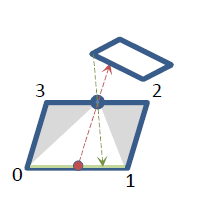
\includegraphics[width=0.35\linewidth]{includes/images/QCar}
\caption{Représentation d'un QCar piloté, tiré de la consigne du projet}
\label{fig:qcar}
\end{figure}
\subparagraph{Déplacements}
La seule action qu'un QCar piloté puisse faire est bouger ou non. Pour cela, il a deux styles de mouvements possibles : les mouvements de surface (ou de côté) et les mouvements d'angle. Ces possibilités sont illustrées sur la figure \ref{fig:qcardepl}
\begin{figure}[h!]
\centering
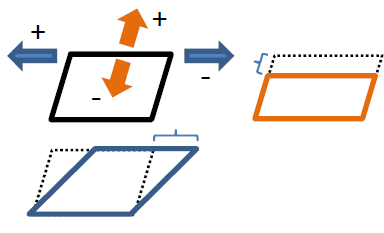
\includegraphics[width=0.4\linewidth]{includes/images/qcar_depl}
\caption{Représentation des mouvements possibles d'un QCar piloté, tiré de la consigne du projet}
\label{fig:qcardepl}
\end{figure}
\subparagraph{Collisions}
Au moment où 2 QCar se touchent (1 côté contre 1 sommet), on considère qu'il y a une collision. Dès lors, si le sommet avait un point, il le perd au profit du second QCar. Et inversement pour le côté. Les collisions se font sans rebonds.
\section{Organisation du projet}
bla
\subsection{Planning}
Au début, nous avions réalisé la planification visible sur la figure \ref{fig:planning}. Au final, cette planification était peut-être trop vague et nous ne l'avons pas exploitée correctement.
\begin{figure}[H]
\centering
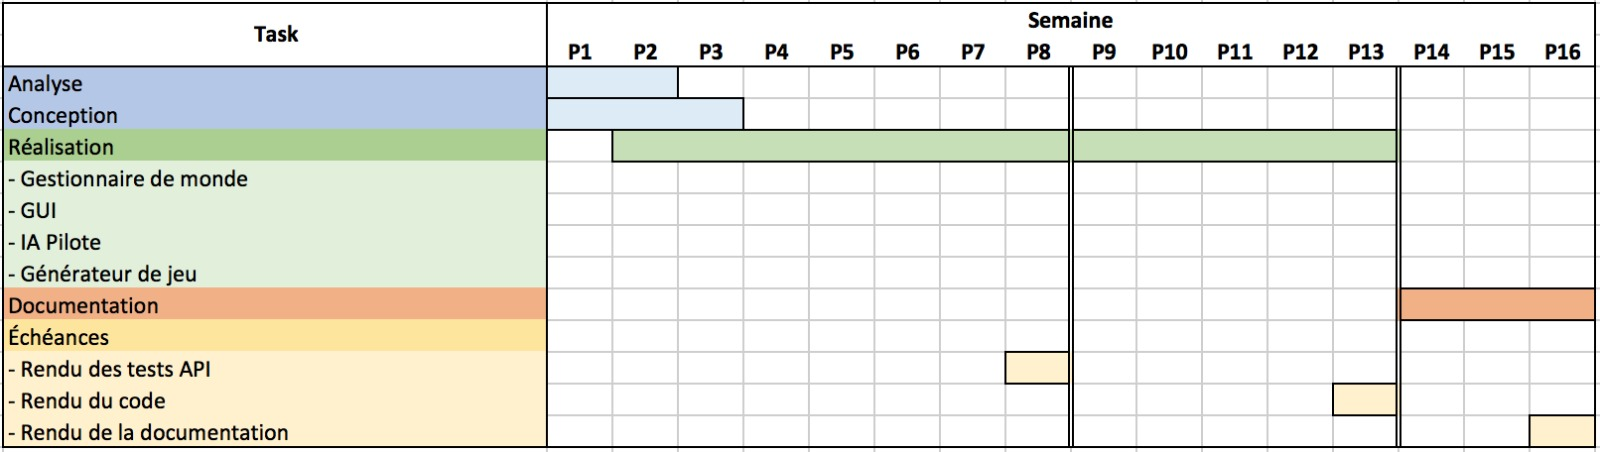
\includegraphics[width=1\linewidth]{includes/images/planning}
\caption{Planification initiale}
\label{fig:planning}
\end{figure}
\subsection{Déroulement}
Chaque semaine, nous essayions de faire une réunion pour faire le point sur les tâches en cours, à faire, et les tâches terminées. Chacun se voyait attribuer des tâches à faire pour la semaine à venir. Malheureusement, notre planification étant trop flexible, nous ne respections pas vraiment les échéances et le suivi des tâches était assez flou.
\subsection{Répartition du travail}
Le travail a été réparti entre les membres du groupe. Un tableau récapitulatif en page \pageref{tabletaches}
\subsection{Gestion du projet}
Pour gérer les taches à faire, celles en cours et celle terminée, nous avons décidé d'utiliser Trello. Cet outil en ligne permet de créer des tâches avec des dates d'échéance, de les déplacer aisément. Cela s'inspire de la méthode SCRUM. Un aperçu de l'interface est visible sur la figure \ref{fig:trello}
\begin{figure}[H]
\centering
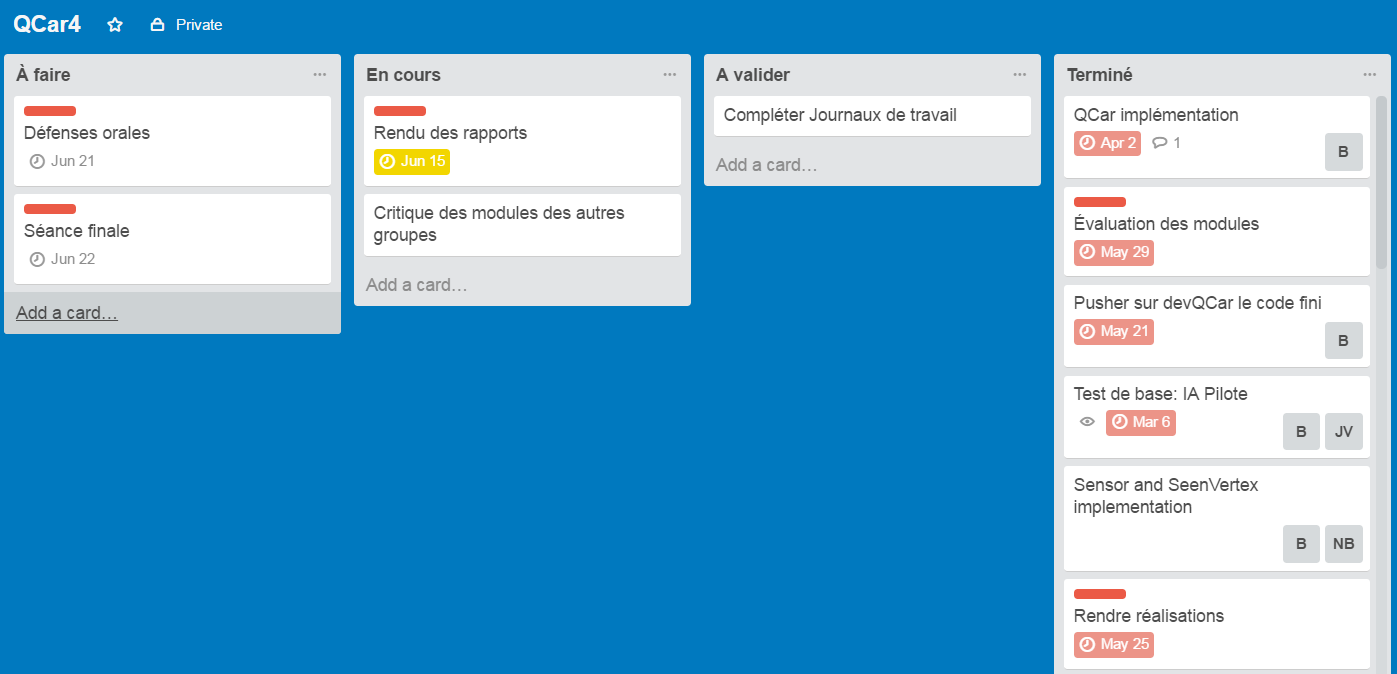
\includegraphics[width=1\linewidth]{includes/images/trello}
\caption{Aperçu de l'interface de Trello}
\label{fig:trello}
\end{figure}
\section{Analyse}
La spécification du projet QCar est très précise en ce qui concerne la structure du projet. La raison de cette précision est que l'étape finale du projet consiste à comparer les réalisations des différents groupes de la classe. Pour que cet objectif soit réalisable, les superviseurs du projet on fournit une "Application Programming Interface" (API) qui régit les interactions entre différents modules de l'application et les rend interchangeables. De plus, deux bibliothèques sont fournies pour aider à réaliser la représentation graphique de l'état du jeu. Contrairement à un projet "from scratch" traditionnel où la phase d'analyse est relativement longue et complexe dans le but de créer une bonne base pour les phases suivantes de la réalisation, la phase d'analyse du projet QCar est axée sur la compréhension des modules fournis. 
\subsection{Analyse de QCar-API} 
L'API QCar définit une découpe modulaire du projet. Chacun des modules principaux peut être accédé par l'intermédiaire d'une classe Factory principale. Ces modules principaux sont le GameProvider, le WorldManager et le Driver. Il y a en réalité un quatrième module principal qui est l'interface graphique, mais il est traité ultérieurement dans cette analyse.
\begin{figure}[H]
 \centering
 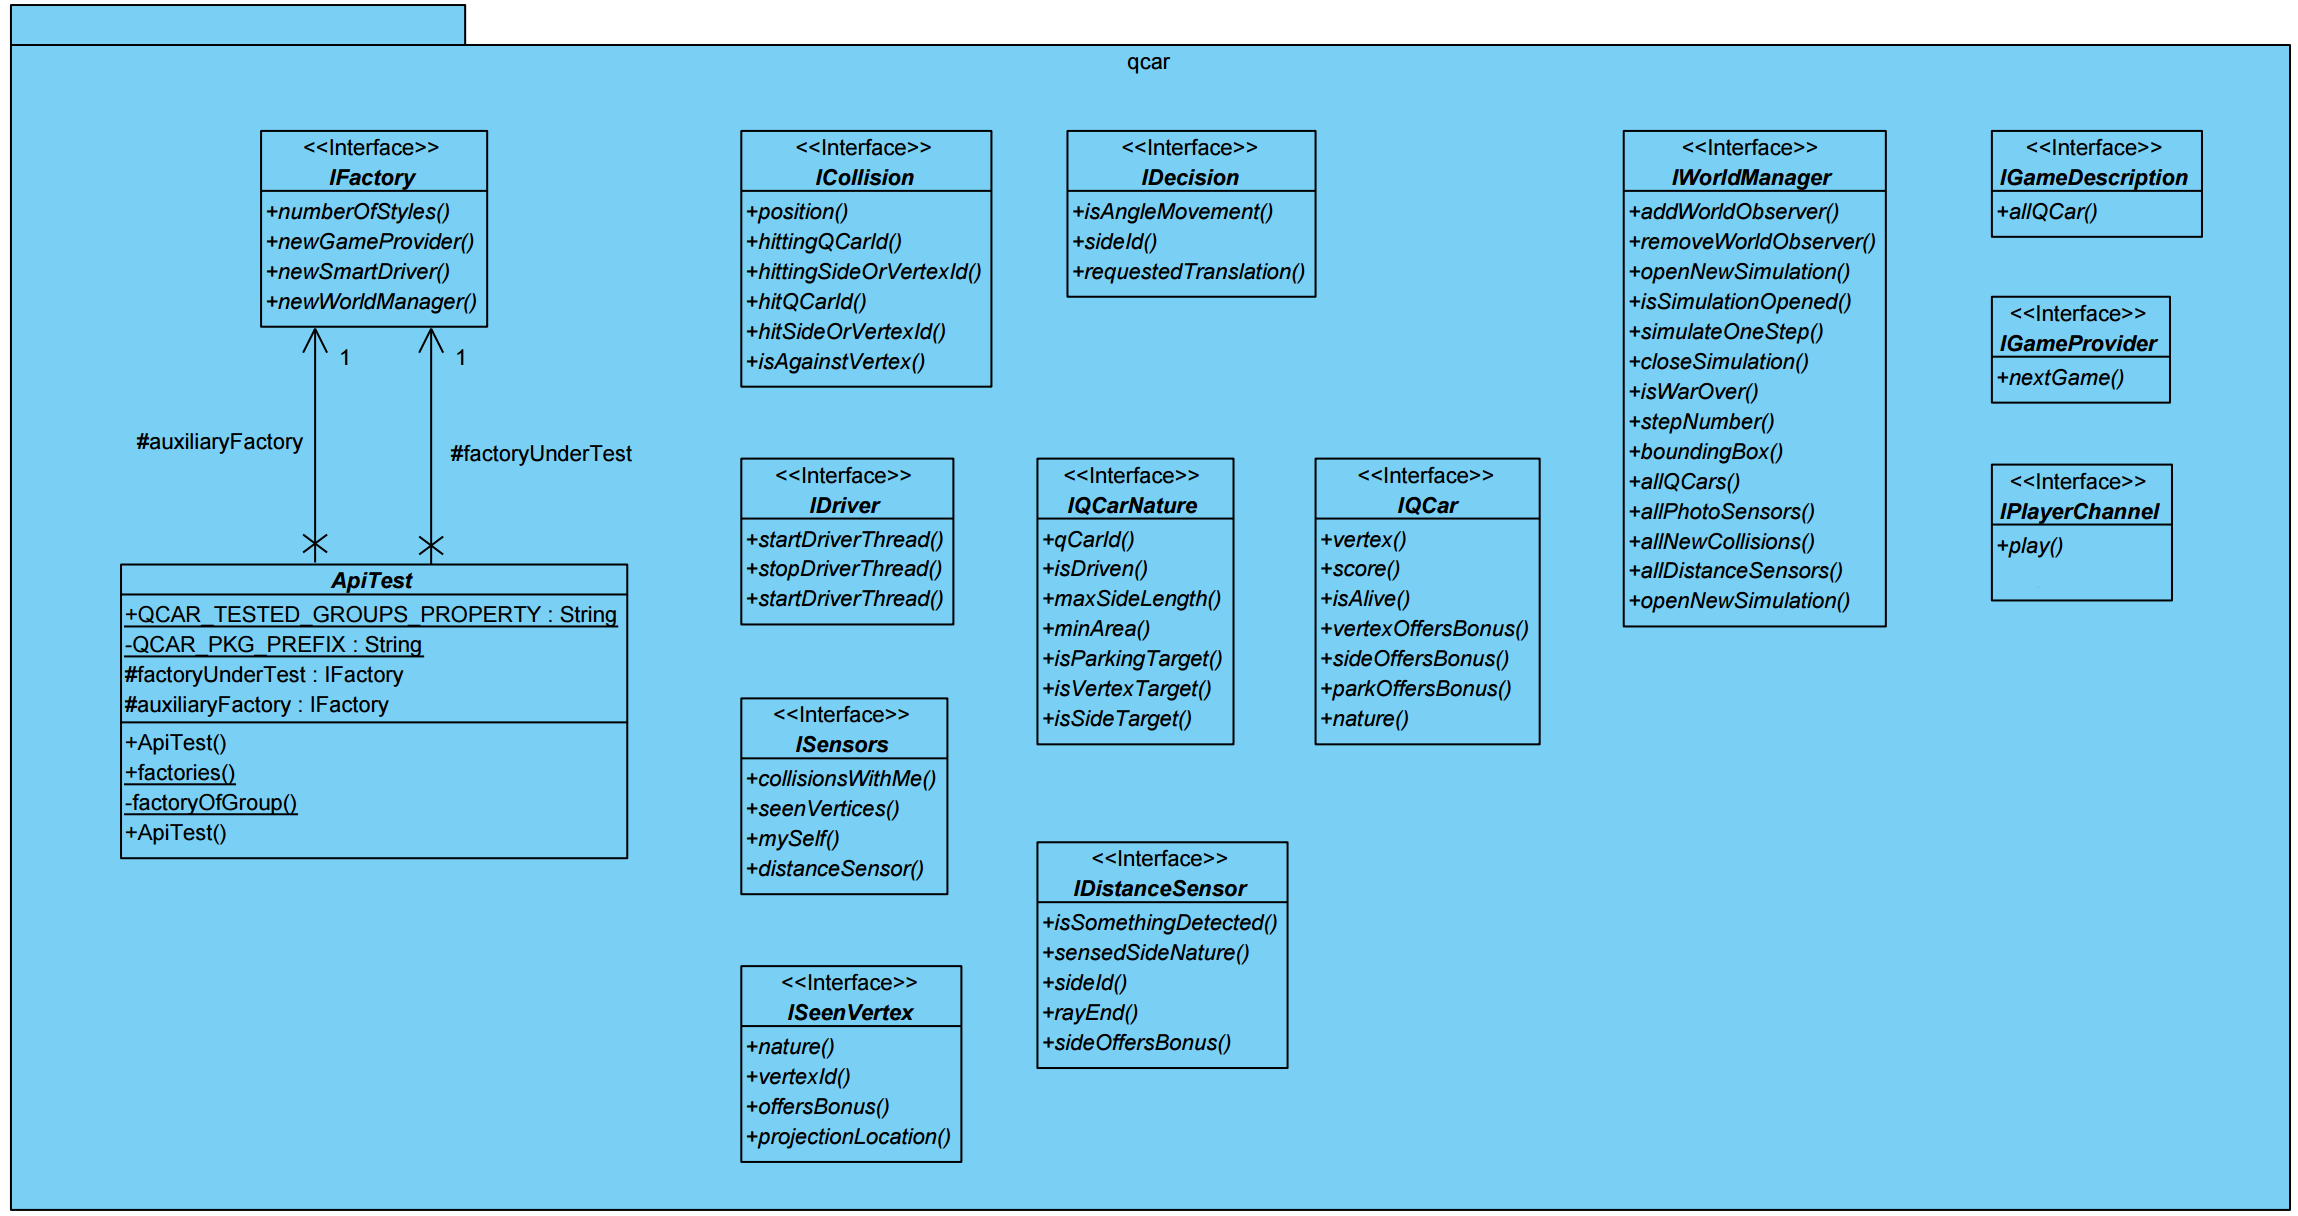
\includegraphics[width=1.0\textwidth]{includes/images/diag_classes_api}
 \caption{\label{fig:diag_classes_api}Diagramme de classes de l'API}
\end{figure}
Chacun des trois modules principaux de l'API possède une interface Java qui lui est dédiée. Les autres interfaces représentent des données qui transitent entre les différents modules.
\paragraph{ICollision}
Les objets implémentant cette interface représentent une collision entre deux QCars.
\paragraph{ISensors}
Les objets implémentant cette interface représentent les senseurs permettant aux Drivers de "voir" le monde et de prendre leurs décisions. Ils regroupent les capteurs photosensibles et les capteurs de distance. Seuls les QCars pilotés ont des senseurs.
\paragraph{ISeenVertex}
Les objets implémentant cette interface représentent un point de QCar qui est vu par le capteur photosensible d'un autre QCar. Le capteur photosensible est un côté particulier du QCar, opposé à un "oeil" qui se trouve entre ses sommets 2 et 3. Le capteur est donc sur le côté inverse, entre les sommets 0 et 1.
\paragraph{IDecision}
Les objets implémentant cette interface représentent une décision prise par un QCar concernant un mouvement. Cette décision sera ensuite interprétée par le WorldManager et provoquera éventuellement de nouvelles collisions et un nouvel état de jeu à transformer en senseurs.
\paragraph{IQCarNature}
Les objets implémentant cette interface représentent la "nature" d'un QCar. Cette nature est comme une carte d'identité pour le QCar et définit une bonne partie de ses attributs.
\paragraph{IDistanceSensor}
Les objets implémentant cette interface représentent le capteur de distance d'un QCar piloté. Ce capteur mesure la distance de l'élément le plus proche avec un rayon, tel un laser, qui part du milieu du capteur photosensible et traverse l'"oeil" du QCar.
\paragraph{IQCar}
Les objets implémentant cette interface représentent un QCar. C'est l'élément principal du jeu qui est représenté comme un parallélogramme. Chaque QCar maintient ses informations internes à jour et met à disposition sa nature.
\paragraph{IGameDescription}
Les objets implémentant cette interface représentent un plateau initial du jeu. Ces objets sont en règle générale fabriqués par un GameProvider et envoyés à un WorldManager.
\paragraph{IPlayerChannel}
Les objets implémentant cette interface représentent un canal de communication entre le WorldManager et un des Drivers de la partie.
\subsection{Analyse de SimViou et QCar-UI}
Les librairies UI et SimViou sont analysées ensemble, car QCar-UI spécialise SimViou. La librairie UI implémente déjà tout ce qui concerne l'affichage du monde. Le fonctionnement de SimViou est détaillé dans sa documentation et n'est pas inclus dans ce rapport. 
\section{Conception}
\subsection{GameProvider}
Le GameProvider sert à créer les QCars de la simulation et à les placer sur le terrain de jeu dans un ordre aléatoire. On peut constater d'emblée que plusieurs contraintes seront à respecter:
\begin{itemize}
 \item le nombre de QCar de nature "driven" est toujours choisi par l'utilisateur de la simulation
 \item aucun QCar ne doit se superposer
 \item aucun QCar ne doit être contenu dans un autre QCar
 \item chaque QCar doit avoir une nature définie
 \item chaque QCar doit respecter une longueur de côté maximale définie
 \item chaque QCar doit respecter une aire minimale définie
 \item l'orientation (angle de rotation par rapport à un point central) et la taille de chaque QCar doivent être choisies de manière aléatoire en tenant compte des contraintes précédentes
\end{itemize}

\subsubsection{Styles}
Les définitions des styles de jeu ont été laissées à l'appréciation de chaque groupe. Ils sont définis dans la classe "GameDescription". Il a été décidé de retenir quatre styles principaux:
\begin{itemize}
 \item un style "MIXED\_STYLE" comprenant à la fois des QCar de nature "driven" contrôlé par une IA "Driver" dont le nombre été choisit par l'utilisateur de la simulation et un mix de QCars de nature "parking" ou "static". Le nombre de ces derniers vaudra une fois et demie le nombre de QCar "driven"
 \item un style "ONLY\_DRIVERS" qui ne comporte que des QCar de nature "driven"
 \item un style "NO\_STATICS" qui ne comporte que des QCar de nature "driven" et "parking"
 \item un style "NO\_PARKING" qui ne comporte que des QCar de nature "driven" et "static"
\end{itemize}
Il est à noter que chacun de ces styles peut être décliné pour un terrain de simulation possédant une bordure définie dans un QCar spécifique ou un terrain n'en possédant pas. Cela fait monter le nombre de styles à un total de huit.
\subsection{Physique et collisions}
Comme cité précédemment, le projet requiert un système de physique permettant de calculer des collisions et des capteurs. Ces calculs sont à réaliser à chaque étape de la simulation et sont un aspect fondamental du bon fonctionnement du reste du projet. Par conséquent, plusieurs idées ont été proposées pour la mise en œuvre de cette partie du projet.
\paragraph{Concept de collisions}
Le principe de collisions est un concept courant dans le monde du jeu vidéo. Une collision n'a pas de sens dans un monde statique, car elle est forcément engendrée par un déplacement (ne serait-ce que de la caméra). Ce principe est très intéressant dans le cadre de ce projet, car dans le monde des QCars, vu que la caméra ne provoque pas de changement de perspective, la seule source de collisions est les mouvements de QCars engendrés par les décisions des Drivers. Ceci permet donc de définir à quel moment les collisions doivent être calculées. De plus, le calcul des collisions à ce moment est crucial, car il permet de bloquer les déplacements qui seraient illégaux. Les QCars ont la capacité de réaliser deux types de mouvements qui sont différenciés par le fait qu'il s'agit ou non d'un mouvement d'angle. Cette différence est à prendre en compte lors de la réalisation du calcul de collisions, bien que suivant la méthode choisie, un des cas est une extension ou une simplification de l'autre.
\paragraph{Démarche}
La complexité de la réalisation d'un système de collisions varie grandement selon les outils utilisés. Dans la suite de ce rapport, trois possibilités de réalisation vont être présentées. Ces trois solutions ne sont pas complètement indépendantes, mais plutôt des itérations de l'idée de base qui permettent de simplifier, optimiser ou clarifier le système de collisions.
\subsubsection{Idée de base: Collisions par intersections}
Bien qu'il y ait beaucoup de manières d'envisager la résolution du problème des collisions, la nature du jeu des QCars fait que l'on retourne toujours à un même concept basique: une collision se produit lorsqu'un point intersecte une droite. 
\subsubsection{Idée 1: Collisions par trigonométrie}
Cette solution se baserait entièrement sur la trigonométrie pour obtenir les distances et les points nécessaires. Cette méthode est intéressante, mais elle fait recours à des outils mathématiques relativement basiques et un traitement plus complexe des cas spéciaux comparé aux autres idées présentées. De plus, elle ne permet aucun type de filtrage ou simplification sur les données à traiter.
\subsubsection{Idée 2: Collisions par changement de base}
Le principe de cette solution utilise les compétences acquises dans les cours d'Algèbre. Le projet QCar utilise une base XY classique. Ce système d'axes est très utile pour une représentation à l'écran, mais rend difficile l'interprétation du résultat de certains calculs qu'il faut réaliser pour les collisions. Pour pallier à ce problème, un changement de base s'avère très utile.
\paragraph{Idée du changement de base}
Changer la base revient à déplacer l'origine du système de coordonnées sur un des points du QCar dont on veut calculer les collisions, à redéfinir l'angle entre les axes et à modifier la graduation des axes pour que le secteur balayé par les mouvements se trouve entre 0 et 1. Ce nouveau système de coordonnées est nommé A1A2.
\begin{figure}[H]
 \centering
 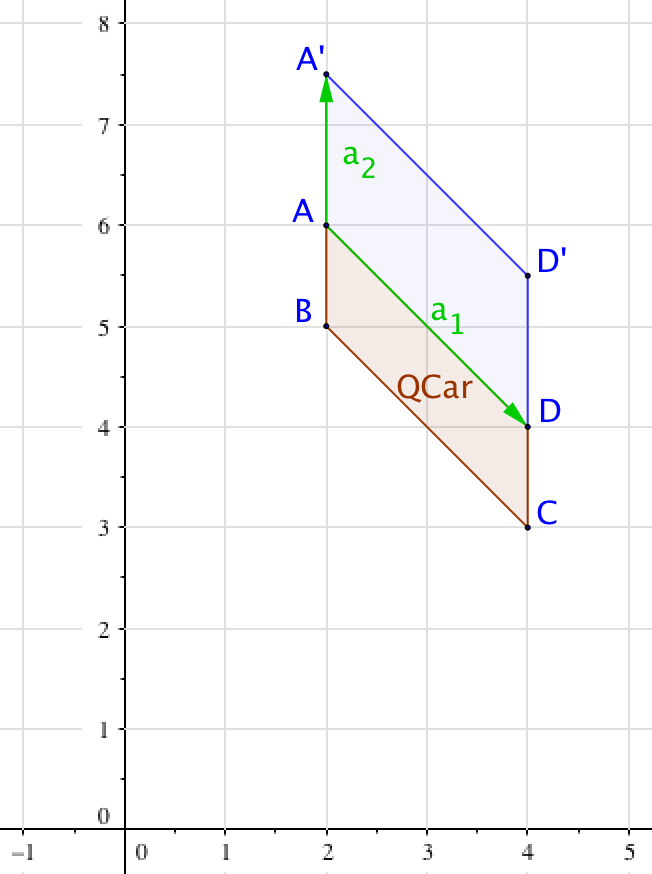
\includegraphics[width=0.5\textwidth]{includes/images/physique_conception_01}
 \caption{\label{fig:physique_conception_01}Représentation des nouveaux axes}
\end{figure}
Comme le montre la Figure \ref{fig:physique_conception_01}, le QCar $ABCD$ (représenté en brun) souhaite déplacer réaliser un déplacement non angulaire de son côté $AD$ vers $A'D'$. Le nouveau système d'axes $a_1a_2$ est ancré sur le point $A$. Le vecteur de base $\overrightarrow{a_1}$ est confondu avec le côté $AD$. Le vecteur $\overrightarrow{a_2}$ est engendré par les points $AA'$. La zone en bleu correspond à la zone de balayage du QCar. Si un point se trouve dans cette zone ou sur son périmètre ses coordonnées transformées seront dans l'intervalle $[0;1]$ pour les deux coordonnées.
\paragraph{Matrice de transition}
Une fois la base du système d'axes A1A2 définie, il est possible de calculer une matrice de passage et sa matrice inverse qui permettent de transformer n'importe quel point exprimé dans la base XY dans la base A1A2 et inversement.
\[
 P =
 \begin{bmatrix}
 ({a_1}_{XY}X2 - {a_1}_{XY}X1) & ({a_2}_{XY}X2 - {a_2}_{XY}X1) \\
 ({a_1}_{XY}Y2 - {a_1}_{XY}Y1) & ({a_2}_{XY}Y2 - {a_2}_{XY}Y1)
 \end{bmatrix}
\]
\[
 P^{-1} = \frac{1}{\det(P)} * 
 \begin{bmatrix}
 P_{11} & -P_{10} \\
 -P_{01} & P_{00}
 \end{bmatrix}
\]
\paragraph{Algorithme selon cette méthode}
Grâce aux matrices de passage, il est possible de rapidement parcourir tous les sommets du jeu et de définir s'ils sont pertinents ou non, car après transformation, une partie des points ayant des coordonnées négatives s'avèrent non pertinents pour les collisions du QCar en cours de traitement. Les points pertinents sont alors testés avec la méthode des intersections.
\begin{figure}[H]
 \centering
 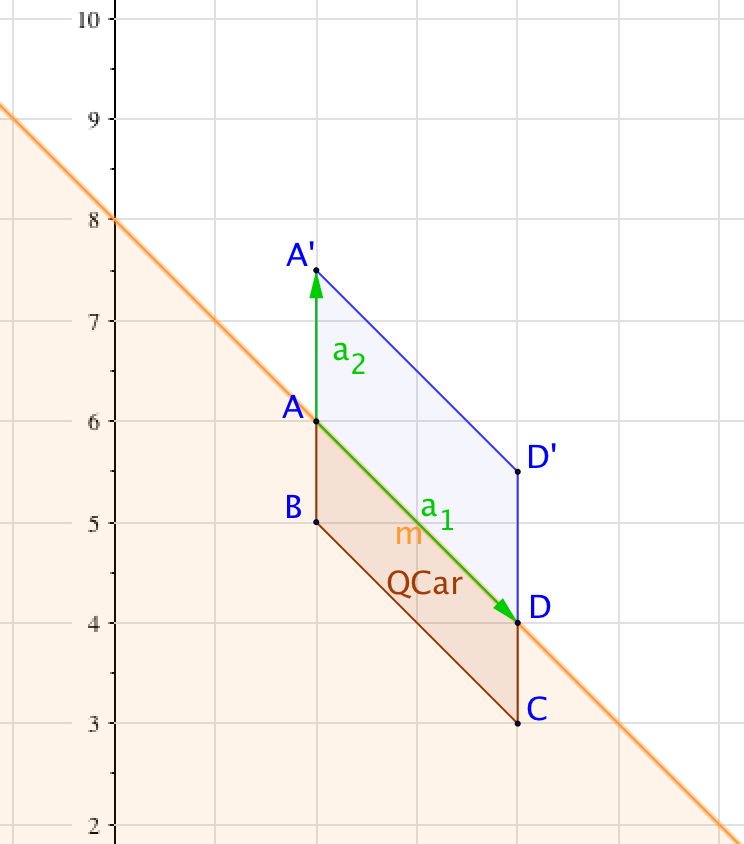
\includegraphics[width=0.5\textwidth]{includes/images/physique_conception_02}
 \caption{\label{fig:physique_conception_02}Représentation des points filtrés}
\end{figure}
Comme le montre la Figure \ref{fig:physique_conception_02}, les points qui se trouvent dans la zone orange sont laissés de côté, car ils ne sont pas pertinents. Selon les déplacements autorisés pour QCar, ces points ne pourraient jamais entrer en collision avec un QCar à ce moment précis de la simulation. Il est impossible de mettre de côté plus de points, car il faut prendre en compte la possibilité que la zone balayée soit traversée par un côté de QCar dont aucun point n'est dans la zone.
\paragraph{Optimisation du parcours des points}
L'optimisation du parcours des points fait l'hypothèse que les points sommets de QCars sont stockés dans une structure de données du type "2-dimensional-rage-tree". Lors du remplissage de cette structure, on profite du parcours de la liste des QCars pour stocker la valeur maximale de toutes les longueurs maximales des côtés des QCars. Lorsqu'il faut appliquer les collisions sur un QCar, on peut prendre uniquement les points qui sont inclus dans une distance comprise entre la coordonnée minimale en x et y moins la distance maximale stockée et la coordonnée maximale en x et y plus la distance maximale stockée. 
\begin{figure}[H]
 \centering
 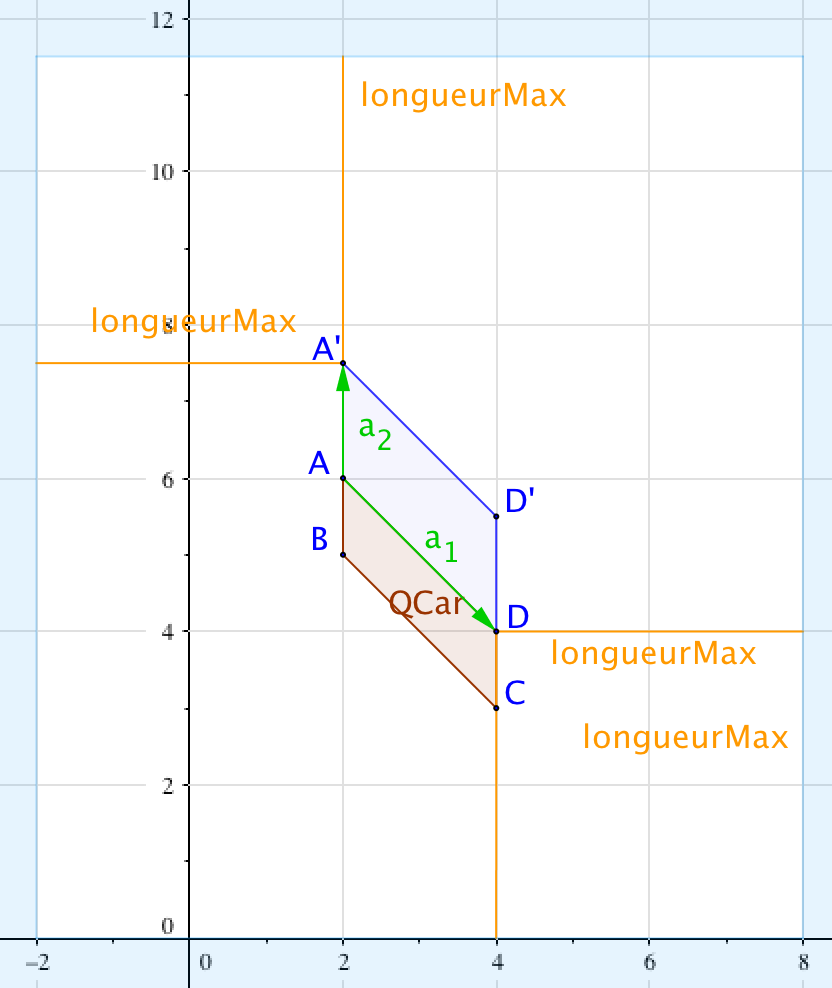
\includegraphics[width=0.5\textwidth]{includes/images/physique_conception_03}
 \caption{\label{fig:physique_conception_03}Représentation de la zone de points à prendre en compte}
\end{figure}
La Figure \ref{fig:physique_conception_03} montre comment le système d'optimisation fonctionne. La mise en place de ce système garantit que tous les points susceptibles d'engendrer une droite qui traverse la zone de déplacement du QCar sont pris en compte. Le filtrage des points pour cette optimisation est réalisé avant la transformation des coordonnées dans la nouvelle base $A_1A_2$. L'idée présentée sur la Figure \ref{fig:physique_conception_02} est appliquée par la suite et a toujours son utilité.
\subsubsection{Idée 3: Ajout d'une grille sur le plan}
Le principe de cette idée est de découper le plan en plusieurs carrés de façon régulière. Puis, pour chaque ligne générant le quadrillage, on stocke les points d'intersection générés par les QCars qui occupent plusieurs carrés. Ceci permet, en faisant l'hypothèse d'une structure contenant tous les points des QCars sous forme triée, de ne considérer que les QCars qui se trouvent ou traversent les zones pertinentes pour chaque déplacement d'un QCar. Ce système de quadrillage résout explicitement le problème des segments qui pourraient traverser un carré sans qu'aucun des points d'extrémité ne soit dans ledit carré. Cette idée devient inutile s'il est possible de garantir que le côté des carrés est plus grand que la valeur maximale de toutes les longueurs maximales de côtés des QCars. Elle retombe alors dans le même cas de figure que l'optimisation citée au point précédent.
\begin{figure}[H]
 \centering
 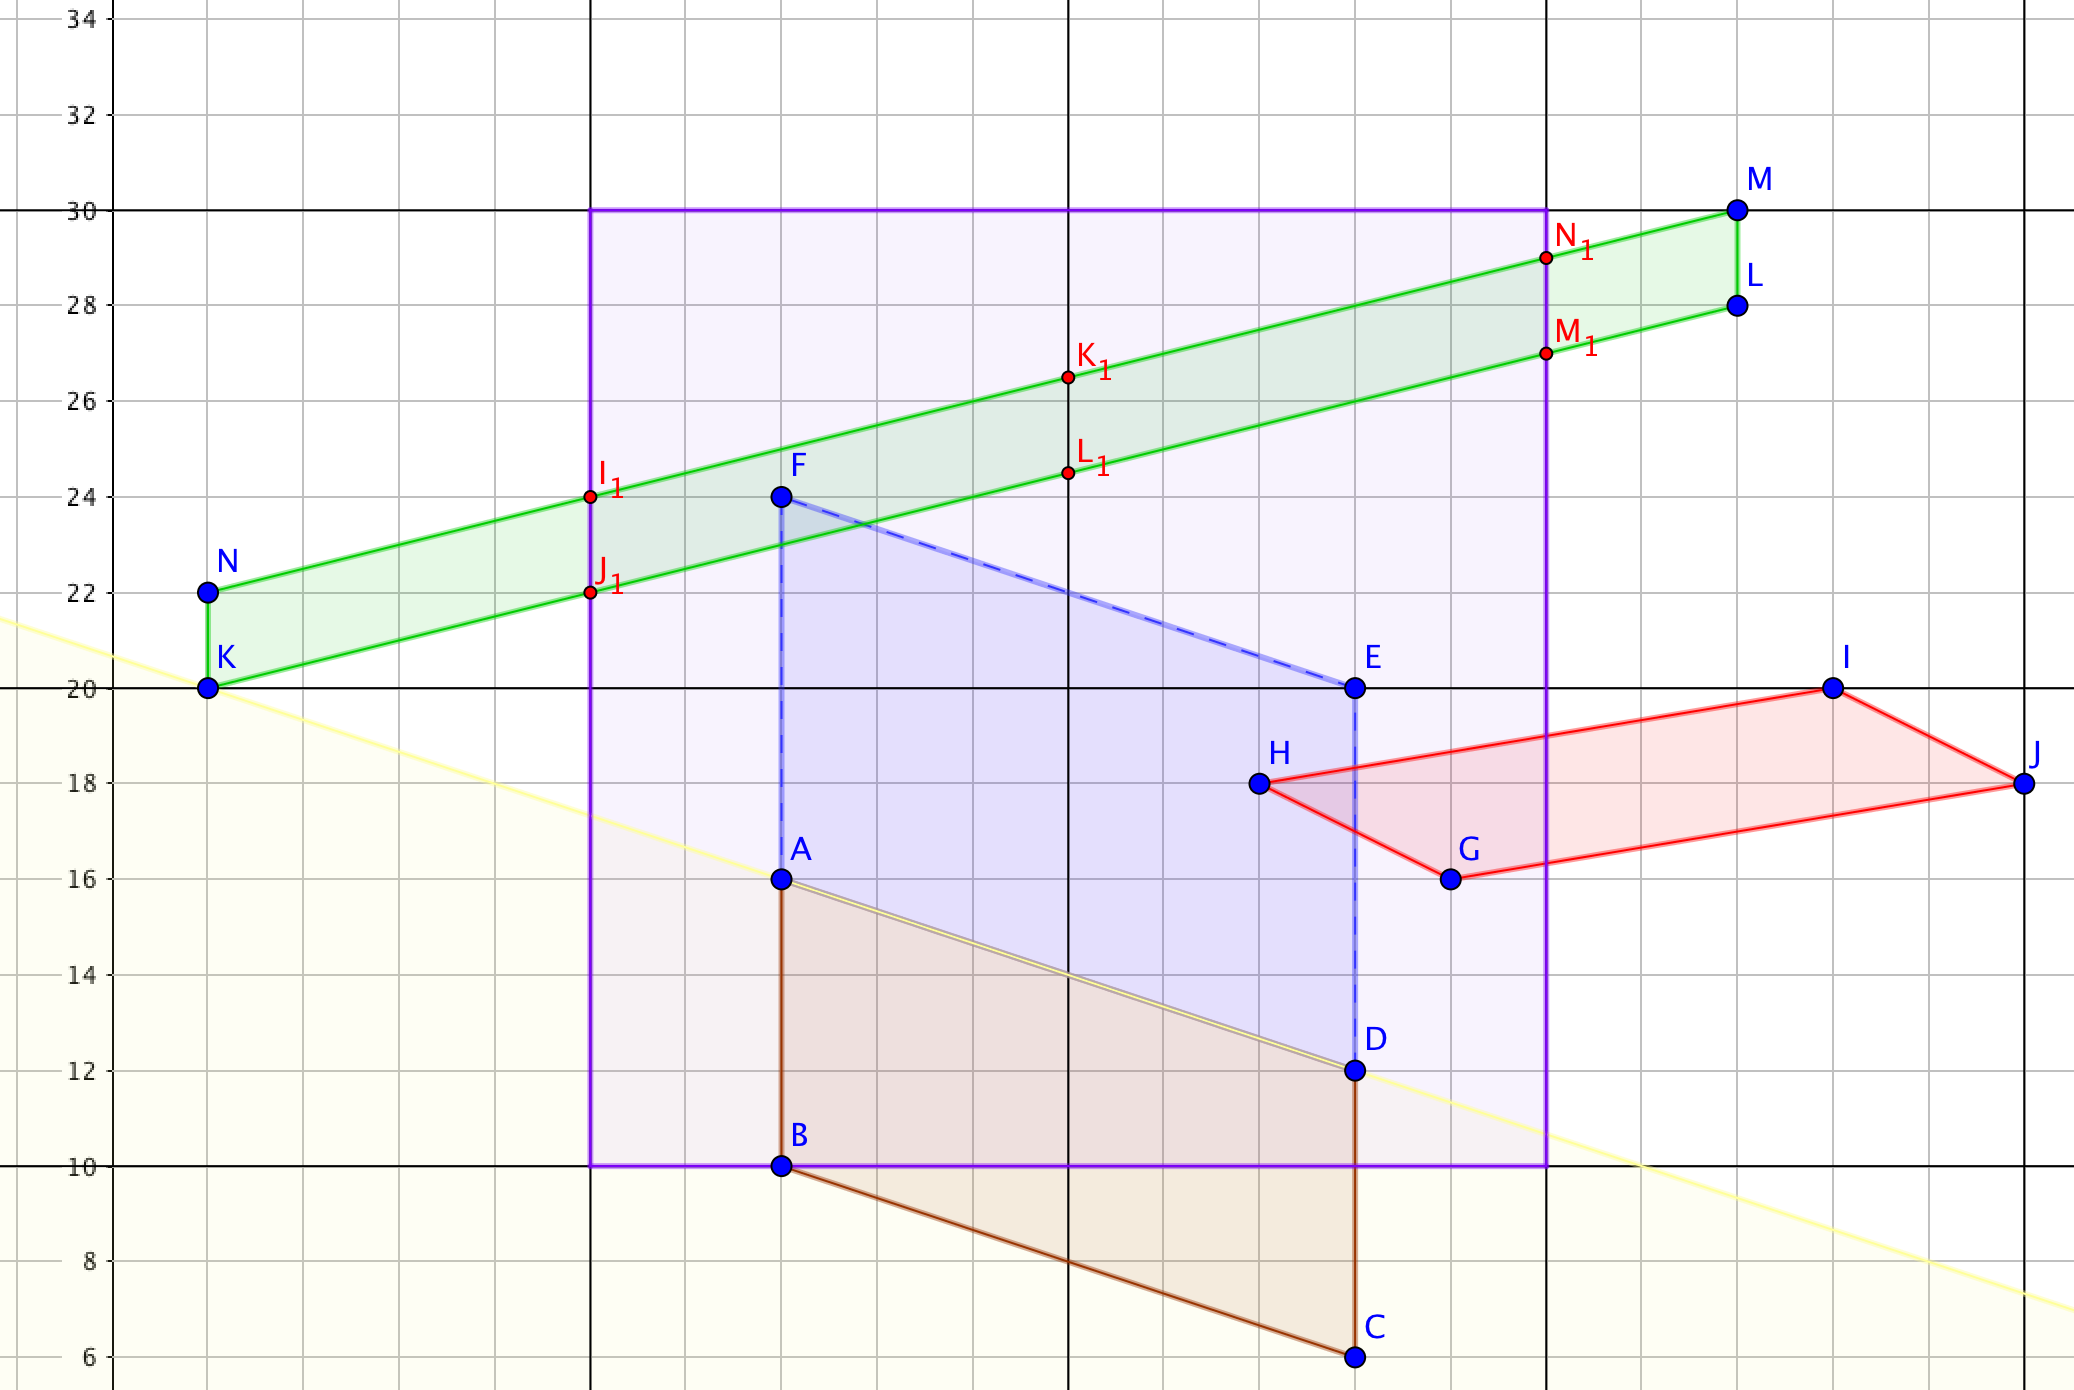
\includegraphics[width=0.7\textwidth]{includes/images/physique_conception_04}
 \caption{\label{fig:physique_conception_04}En rouge, les points intermédiaires stockés}
\end{figure}
La figure 4 montre l'utilité possible d'un tel système. On retrouve une situation du jeu des QCars avec une grille formée par des droites toutes les dix unités du plan. Dans cette figure, le QCar $ABCD$ se prépare à un déplacement en déplaçant le côté $AD$ sur le côté $FE$. La zone en bleu représente la surface parcourue lors du déplacement. La zone en violet représente les zones du grillage qui sont impactées par le déplacement en question, car elles contiennent le QCar en cours de traitement. Le QCar rouge serait facilement détecté, car son sommet $h$ se trouve dans la surface de balayage. Si on néglige la présence du QCar $GHIJ$, la prochaine collision est celle avec le QCar $KLMN$. Cependant, celle-ci n'est pas facile à détecter, car les points ne sont pas dans la zone de balayage. Lors de la génération du quadrillage, les points en rouge $I_1, J_1, K_1, L_1, M_1, N_1$ sont créés et permettent de prendre en compte la présence du QCar $KLMN$, bien que ses sommets ne soient pas dans la zone violette. Cette solution fonctionne bien dans les cas ou le déplacement est aligné avec le quadrillage. Cependant, si le QCar est de travers ou qu'il s'agit d'un déplacement d'angle, cette solution ne s'avère pas très utile et compliquerait l'implémentation. Elle ne sera donc pas utilisée.
\subsubsection{Choix final}
Le choix final pour l'implémentation des collisions se porte sur l'idée 2. Ce choix repose sur le fait qu'elle propose le meilleur compromis entre efficacité, facilité d'implémentation et clarté. L'idée 3 en particulier rajoute beaucoup de complexité dans un projet qui n'en a pas besoin. Si l'ordre de grandeur du nombre total de QCars devait augmenter de manière significative, la mise en place de l'idée 3 pourrait apporter un gain significatif dans les performances de chaque itération.
\subsubsection{Généralisation}
Le même système mis en place pour la détection peu être utilisé pour le calcul des capteurs photo et distance.
\subsection{WorldManager}
Le World manager devra implémenter tout ce qui concerne la gestion du monde. Il est indépendant de l'IHM. Il devra communiquer avec les Drivers via les PlayerChannel. Il faudra implémenter les méthodes pour communiquer avec l'IHM. En plus des méthodes d'accès aux attributs (différentes listes de QCar, Senseurs, Collisions, etc), Il faut les initialiser dans openNewSimulation. C'est aussi le WorldManager qui se charge de détecter si la partie est terminée. La méthode simulateOneStep devra calculer tous les déplacements décidés par les drivers ainsi que les collisions et mettre à jour l'état de ses attributs.
\subsection{PlayerChannel}
Pour la conception du PlayerChannel, en nous basant sur les informations données dans la consigne, nous sommes arrivés au pseudo code suivant : 
\begin{lstlisting}
For each step :
  The World manager sends the sensors
  The World manager releases the driver thread
  The driver takes a decision
  The driver gets locked until next step
  The World Manager retrieves the decision
\end{lstlisting}
A chaque pas de la simulation, le WorldManager va placer les nouveaux senseurs dans chaque PlayerChannel puis il va libérer chaque driver afin de les laisser prendre leur Decision. Une fois que le driver a choisi un mouvement, il va venir se mettre en attente dans le PlayerChannel et le WorldManager va pouvoir récupérer les décisions.
\subsection{Decision}
L'interface IDecision comporte simplement les méthodes d'accès aux attributs. Celles-ci seront implémentées. On ajoutera également une méthode "filtre". Cette méthode devra "valider" une décision. En fonction d'une décision et d'un QCar, elle renverra la décision telle quelle si elle est correcte (du point de vue des nouvelles dimensions du QCar après application de la décision) et corrigera la décision pour la rendre correcte dans le cas contraire. Comme il y a 2 sortes de mouvements possibles, on a différentes contraintes à respecter suivant le mouvement (angleMovement ou non). 
\subsubsection{Approche mathématique} 
\paragraph{Angle movement} Dans ce cas, on cherche à déterminer le déplacement d'angle maximal (décalage d'un côté) qui respectera la contrainte du maxSideLength de la nature du QCar.
\begin{figure} [h!]
\centering
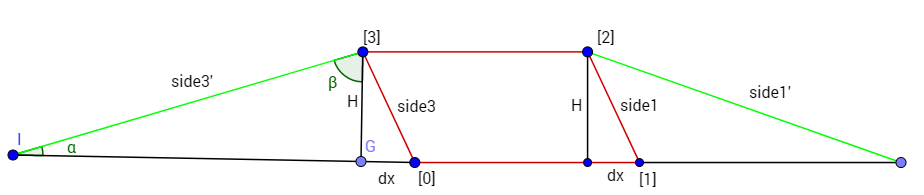
\includegraphics[width=0.9\linewidth]{includes/images/decisions_angle_movement}
\caption{Illustration des contraintes du déplacement d'angle}
\label{fig:decisionsanglemovement}
\end{figure}
Pour illustrer le problème, on va considérer un mouvement du côté 0. Sur la figure \ref{fig:decisionsanglemovement}, c'est le côté du bas. La contrainte sera pour un mouvement positif (vers la droite du dessin) que side1' soit < maxSideLength et pour un mouvement négatif (vers la gauche du dessin) que side3' soit < maxSideLength. On cherche l'allongement maximal du côté 0, donc on cherche la base du triangle rectangle (segment IG sur la figure \ref{fig:decisionsanglemovement}) avec comme hypoténuse side3' = maxSideLength (mSL) et le coté H. On a alors : \[ IG = cos\left(\alpha\right) \cdot mSL = sin\left(\beta\right) \cdot mSL \]
\[ sin\left(\alpha\right) = \frac{H}{mSL} = cos\left(\beta\right) \]
\[ IG = cos\left(arcsin\left(\frac{H}{mSL}\right)\right) \cdot mSL \]
Afin d'ajuster la décision en fonction de l'inclinaison du QCar, il faut ajouter ou enlever dx à la longueur trouvée pour le déplacement maximal.
\[dx = \sqrt{side3^2-H^2}\]
Pour déterminer dans quel "sens" est penché le QCar, on compare la longueur des diagonales (02) et (13). On a les relations suivantes : 
\[(02)>(13) \Rightarrow "droite" \Rightarrow -dx\] 
 \[(02)<(13) \Rightarrow "gauche" \Rightarrow +dx\] 
 \[(02)=(13) \Rightarrow "rectangle" \Rightarrow +-0\] 
 \paragraph{Side movement} Le mouvement d'un côté du QCar est divisé en 2 cas : l'agrandissement  ou la réduction du QCar. On va commencer par la réduction. 
 \paragraph{Side movement négatif}
 \begin{figure}[h!]
\centering
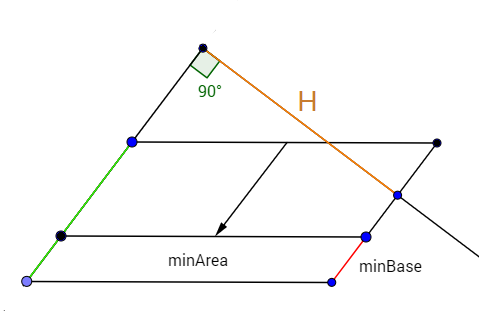
\includegraphics[width=0.6\linewidth]{includes/images/QCar_reduc}
\caption{Illustration des contraintes d'un déplacement de côté négatif}
\label{fig:qcarreduc}
\end{figure}
Sur la figure \ref{fig:qcarreduc}, on illustre un mouvement de côté négatif du côté 3. On a accès à plusieurs longueurs intéressantes : la longueur du côté latéral (side3, en vert sur la figure), et l'aire minimale définie par la nature du QCar : minArea. En calculant la hauteur, on peut trouver minBase à l'aide de la formule de l'aire d'un parallélogramme :
\[minArea = minBase \cdot H  \Rightarrow \frac{minArea}{H} = minBase \]
Le déplacement négatif maximum autorisé vaut donc : $side3 - minBase$
\paragraph{Side movement positif} Le calcul pour un side movement positif est extrêmement simple. Pour calculer le déplacement maximal autorisé, (illustré sur la figure \ref{fig:qcaraugment}), il faut avoir accès à la longueur du côté adjacent à celui qui subit le mouvement (actualSize) et la formule est :\[maxDepl = maxSideLength - actualSize\]
\begin{figure}[h!]
\centering
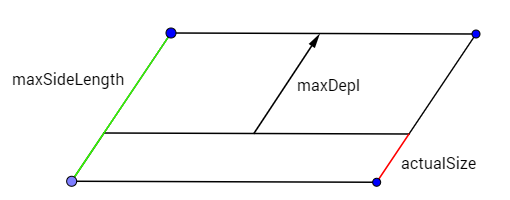
\includegraphics[width=0.7\linewidth]{includes/images/QCar_augment}
\caption{Illustration des contraintes d'un déplacement de côté positif}
\label{fig:qcaraugment}
\end{figure}

\subsection{Driver}
L'interface IDriver nous demande de définir deux méthodes publiques pour le driver : une pour démarrer le processus du pilot et une pour l'arrêter. La prise de décision doit également être implémentée au sein du driver, mais la transmission des informations entre le WorldManager et le driver (décisions et senseurs) est faite via le PlayerChannel
\subsection{IHM}
Pour concevoir l'interface graphique de notre projet, nous avons dans un premier temps lister les éléments que nous avons jugés essentiels afin de voir autour de quels composants notre vue sera articulée. Nous sommes arrivés à la liste suivante:
\begin{itemize}
  \item Sélection du style
  \item Sélection du nombre de Qcar
  \item Classement des QCars dans la partie actuelle
  \item QCarAnimationPane
  \item Panneau de logs
  \item Boutons de contrôle de la partie
  \item Boutons de contrôle manuel du QCar
\end{itemize}
À partir de cette liste, nous avons séparé notre IHM en trois vues: l'éditeur de partie, la simulation et le contrôle manuel d'un QCar. A l'aide de l'outil Balsamiq, nous avons réalisé des maquettes pour nos différentes vues qui ont été ensuite validées lors de nos réunions.
\begin{figure}[H]
 \centering
 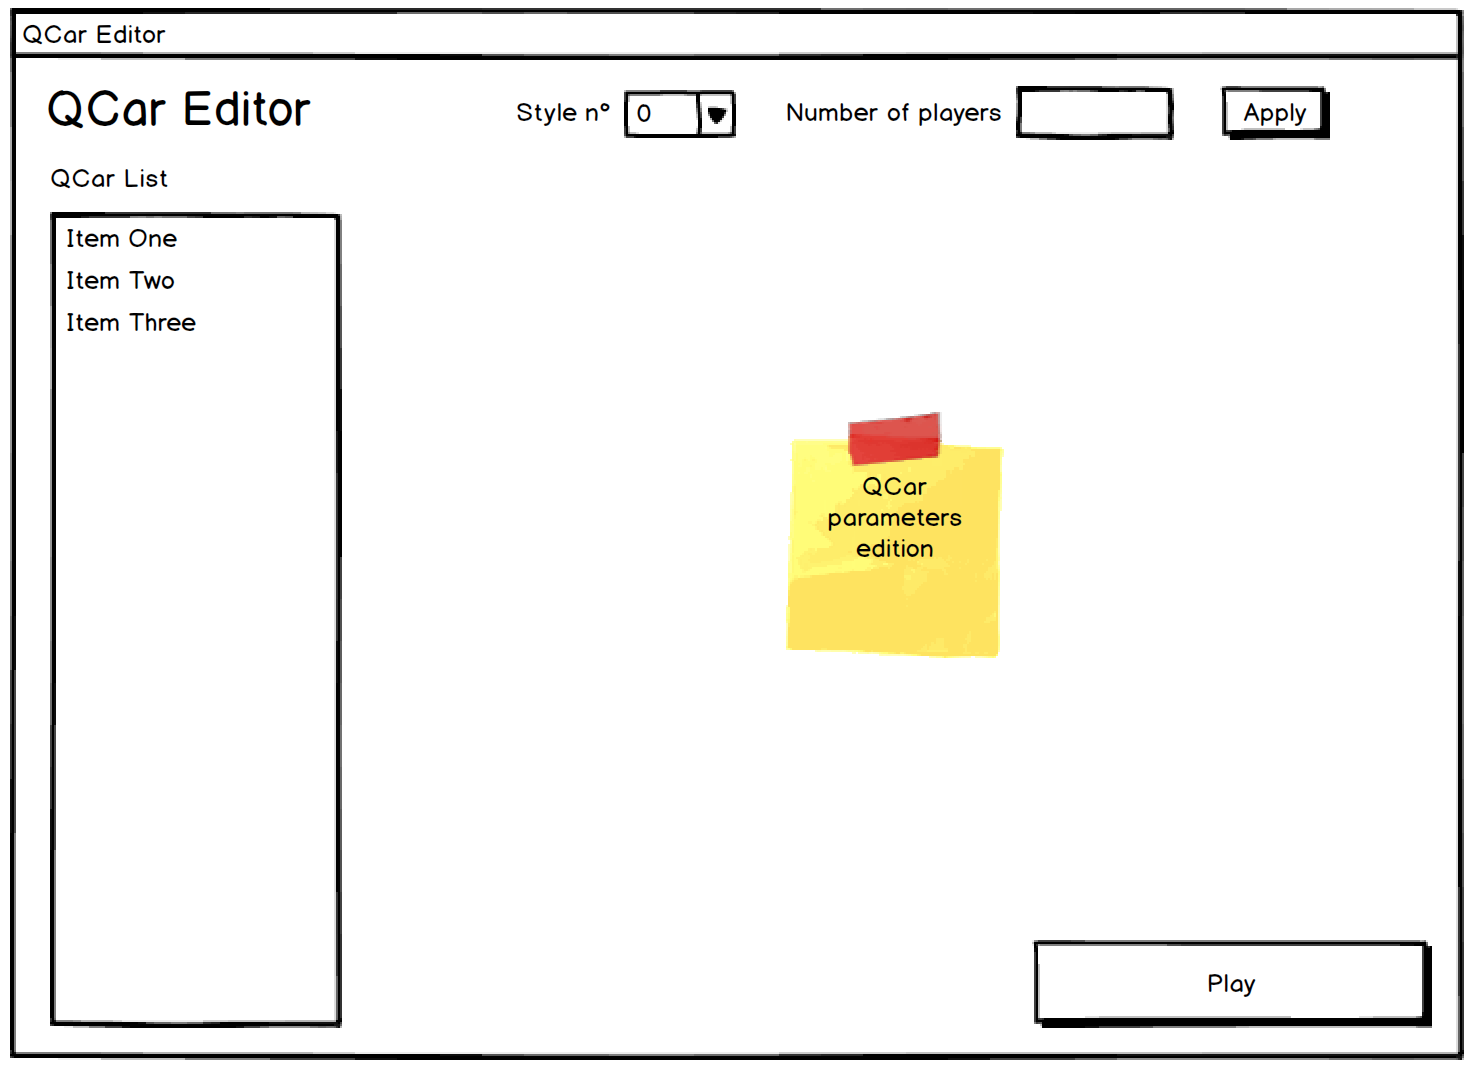
\includegraphics[width=0.7\textwidth]{includes/images/mockupeditor}
 \caption{\label{fig:maquette_editeur}Maquette de l'éditeur de simulation}
\end{figure}
La vue "QCar Editor" est la vue initiale de notre application. Une Combobox permet de sélectionner le numéro du style voulu et un TextField permet de sélectionner le nombre de QCars piloté pour la simulation. Lorsqu'on presse le bouton "Apply", les QCars générés seront placés dans la liste. Si l'utilisateur clique sur un QCar de la liste, les informations de ce QCar seront affichées et si ce QCar est piloté, une Checkbox permettra de prendre le contrôle manuel de ce QCar. Lorsque le bouton "Play" est pressé, la simulation s'ouvre et on passe à la vue suivante.
\begin{figure}[H]
 \centering
 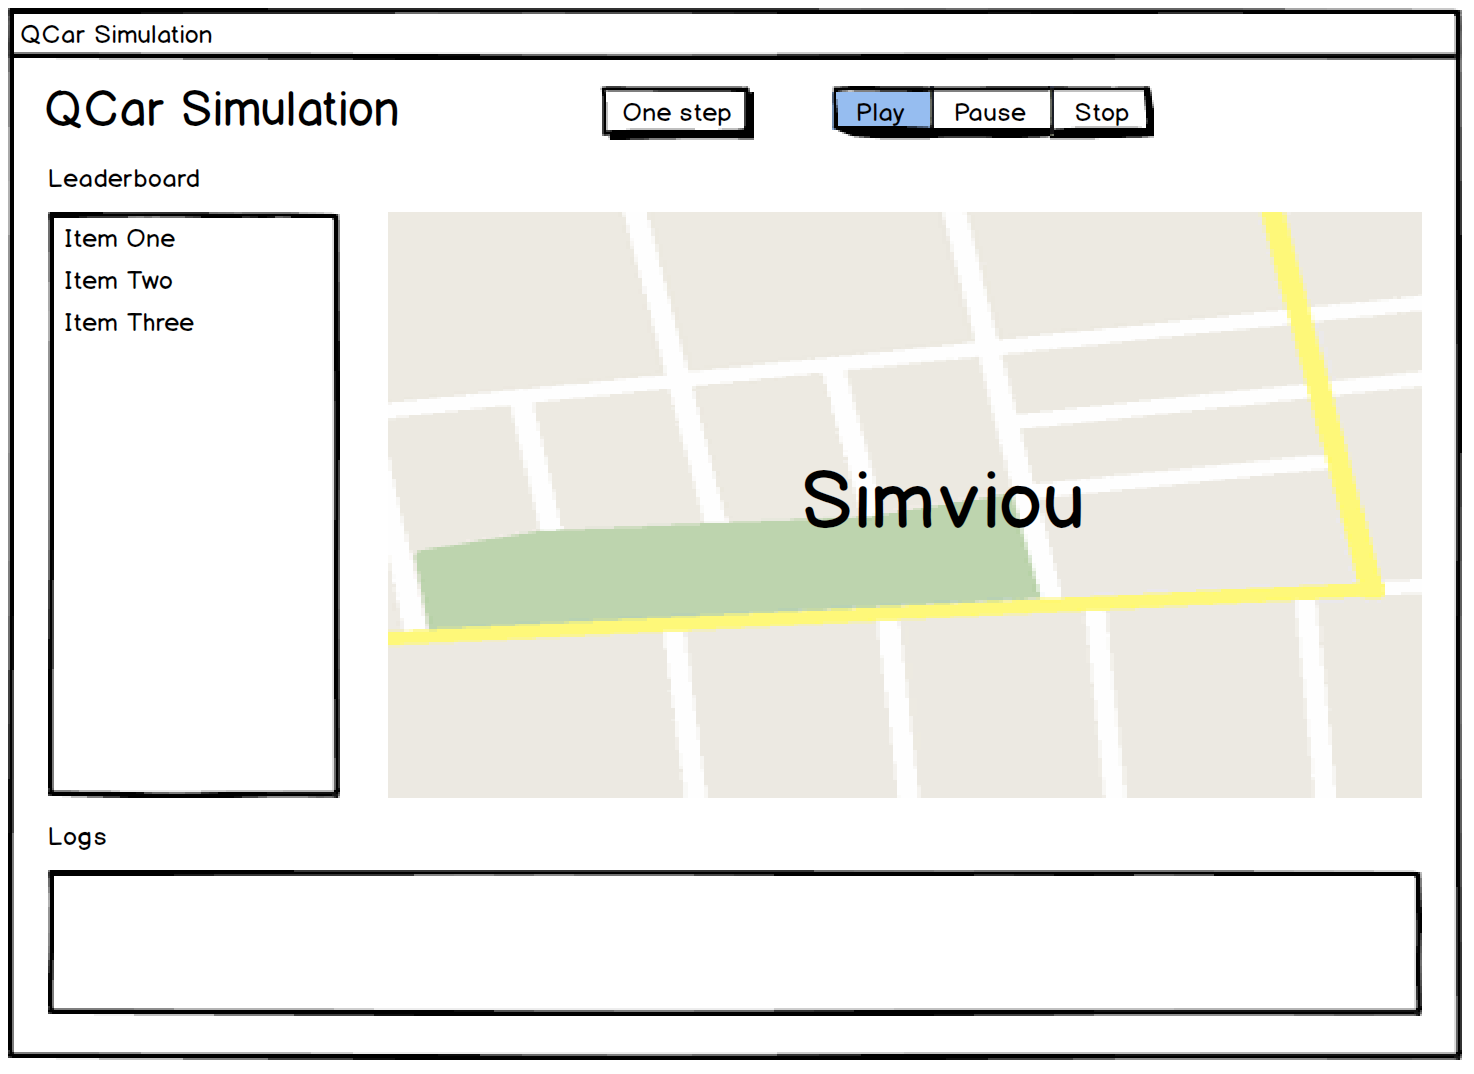
\includegraphics[width=0.7\textwidth]{includes/images/mockupsim}
 \caption{\label{fig:maquette_simulation}Maquette de la simulation}
\end{figure}
C'est dans cette vue que va se dérouler la simulation. Elle contient le QCarAnimationPane qui est la représentation du monde où les QCars évoluent, un classement des QCars pilotés selon leur score, un panneau permettant de logger les événements ainsi que des boutons qui permettent de contrôler la simulation. Une interaction intéressante serait de zoomer sur un QCar lorsqu'on le sélectionne dans le classement.
\begin{figure}[H]
 \centering
 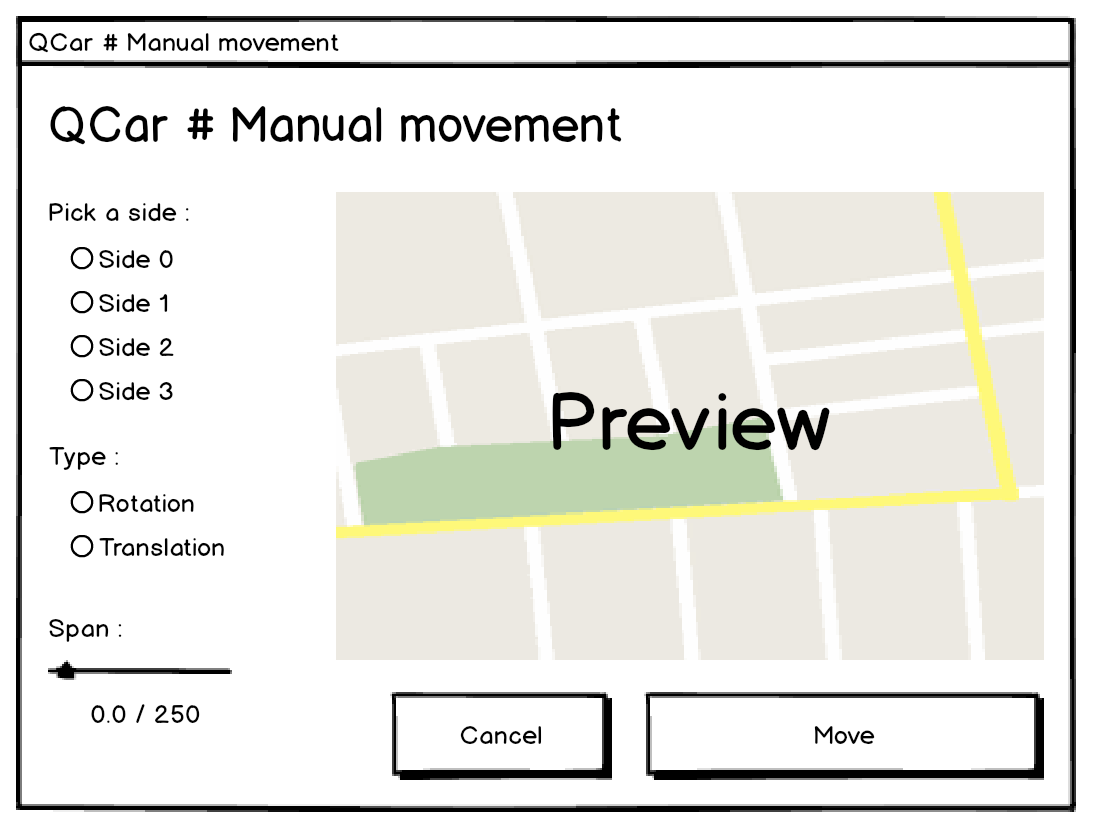
\includegraphics[width=0.7\textwidth]{includes/images/mockupcontrol}
 \caption{\label{fig:maquette_controle}Maquette du pilote manuel du QCar}
\end{figure}
Cette vue sera utilisée uniquement lorsqu'un QCar est contrôlé manuellement et accompagnera la vue de la simulation dans une seconde fenêtre. Elle contient une prévisualisation du mouvement à appliquer ainsi que les options nécessaires aux déplacements du QCar. Le bouton "Move" appliquera le mouvement et le bouton "Cancel" réinitialisera les paramètres du mouvement de manière à avoir un mouvement nul.
Nous avons aussi réfléchi à des interactions telles que des tooltips ou des raccourcis clavier à intégrer à notre projet. Voici une liste des idées que nous avons eu :
\begin{itemize}
  \item Tooltip affichant les informations d'un QCar (nature, score ...) lorsqu'on clique sur un QCar dans la simulation.
  \item Raccourci clavier permettant d'afficher ou non la grille sur le plateau de jeu
  \item Raccourci clavier permettant de mute ou demute l'application
\end{itemize}

\section{Implémentation}
\subsection{GameProvider}
Le principal problème relevé durant la création des QCar est le suivant: assurer que les QCars ne se chevauchent pas.
\subsubsection{Éviter les collisions et chevauchements}
Le principe de base pour la vérification et l'attribution des coordonnées pour les sommets des QCars est de subdiviser l'aire de jeu avec un quadrillage de longueur égale à :
\[ tol * 2 + MAX\_SIDE\_LENGTH \]
avec $ {MAX\_SIDE\_LENGTH} $ étant la longueur maximale du côté d'un QCar et $ {tol} $ étant une tolérance choisie telle que:
\[ tol = MAX\_SIDE\_LENGTH * 0.01 \]
La tolérance $ {tol} $ est ajoutée afin qu'une subdivision du quadrillage ne puisse pas avoir un QCar qui lui soit exactement égal (i.e que les sommets d'un QCar ne puissent pas tous se retrouver sur une intersection du quadrillage).
\begin{figure}[h!]
 \centering
 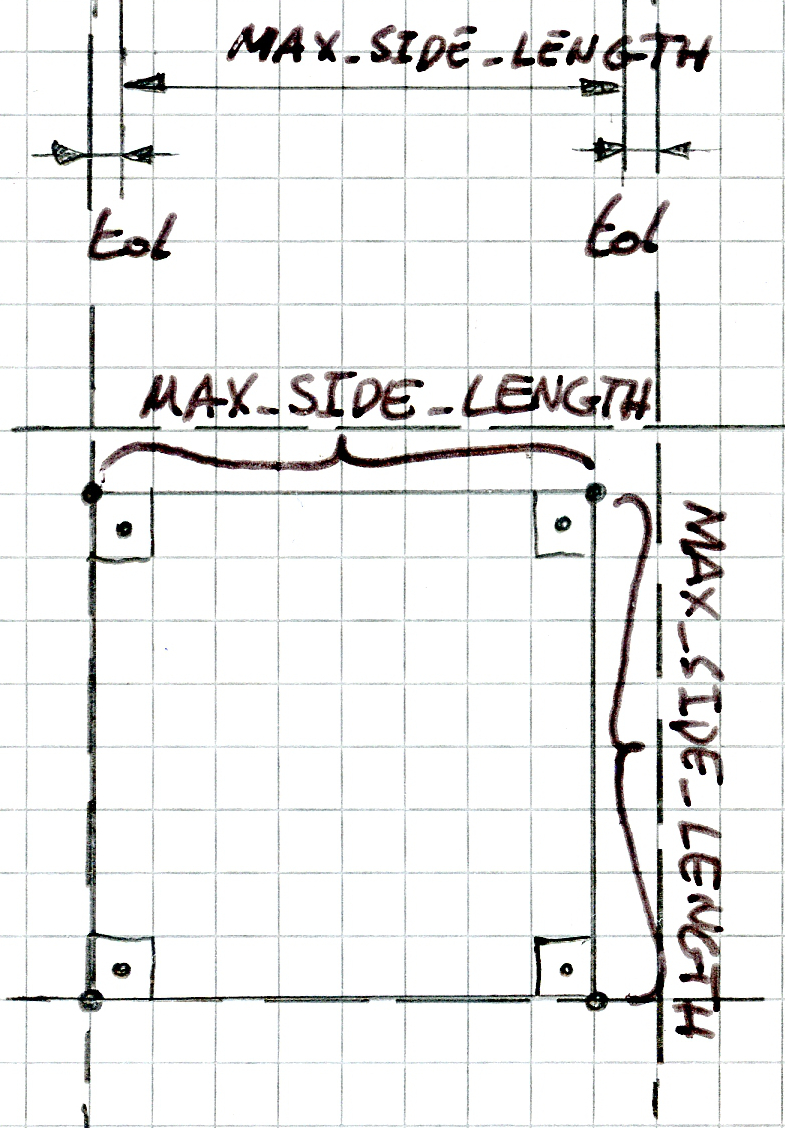
\includegraphics[width=0.25\linewidth]{includes/images/quadri2}
 \caption{Coïncidence entre sommets et subdivisions}
 \label{fig:quadri2}
\end{figure}
L'occupation du quadrillage sera symbolisée par un tableau de valeurs booléennes. L'occupation maximale du quadrillage par un QCar sera de maximum trois subdivisions en x et de trois subdivisions en y en raison de la longueur maximale du côté d'un QCar.
\begin{figure}[h!]
 \centering
 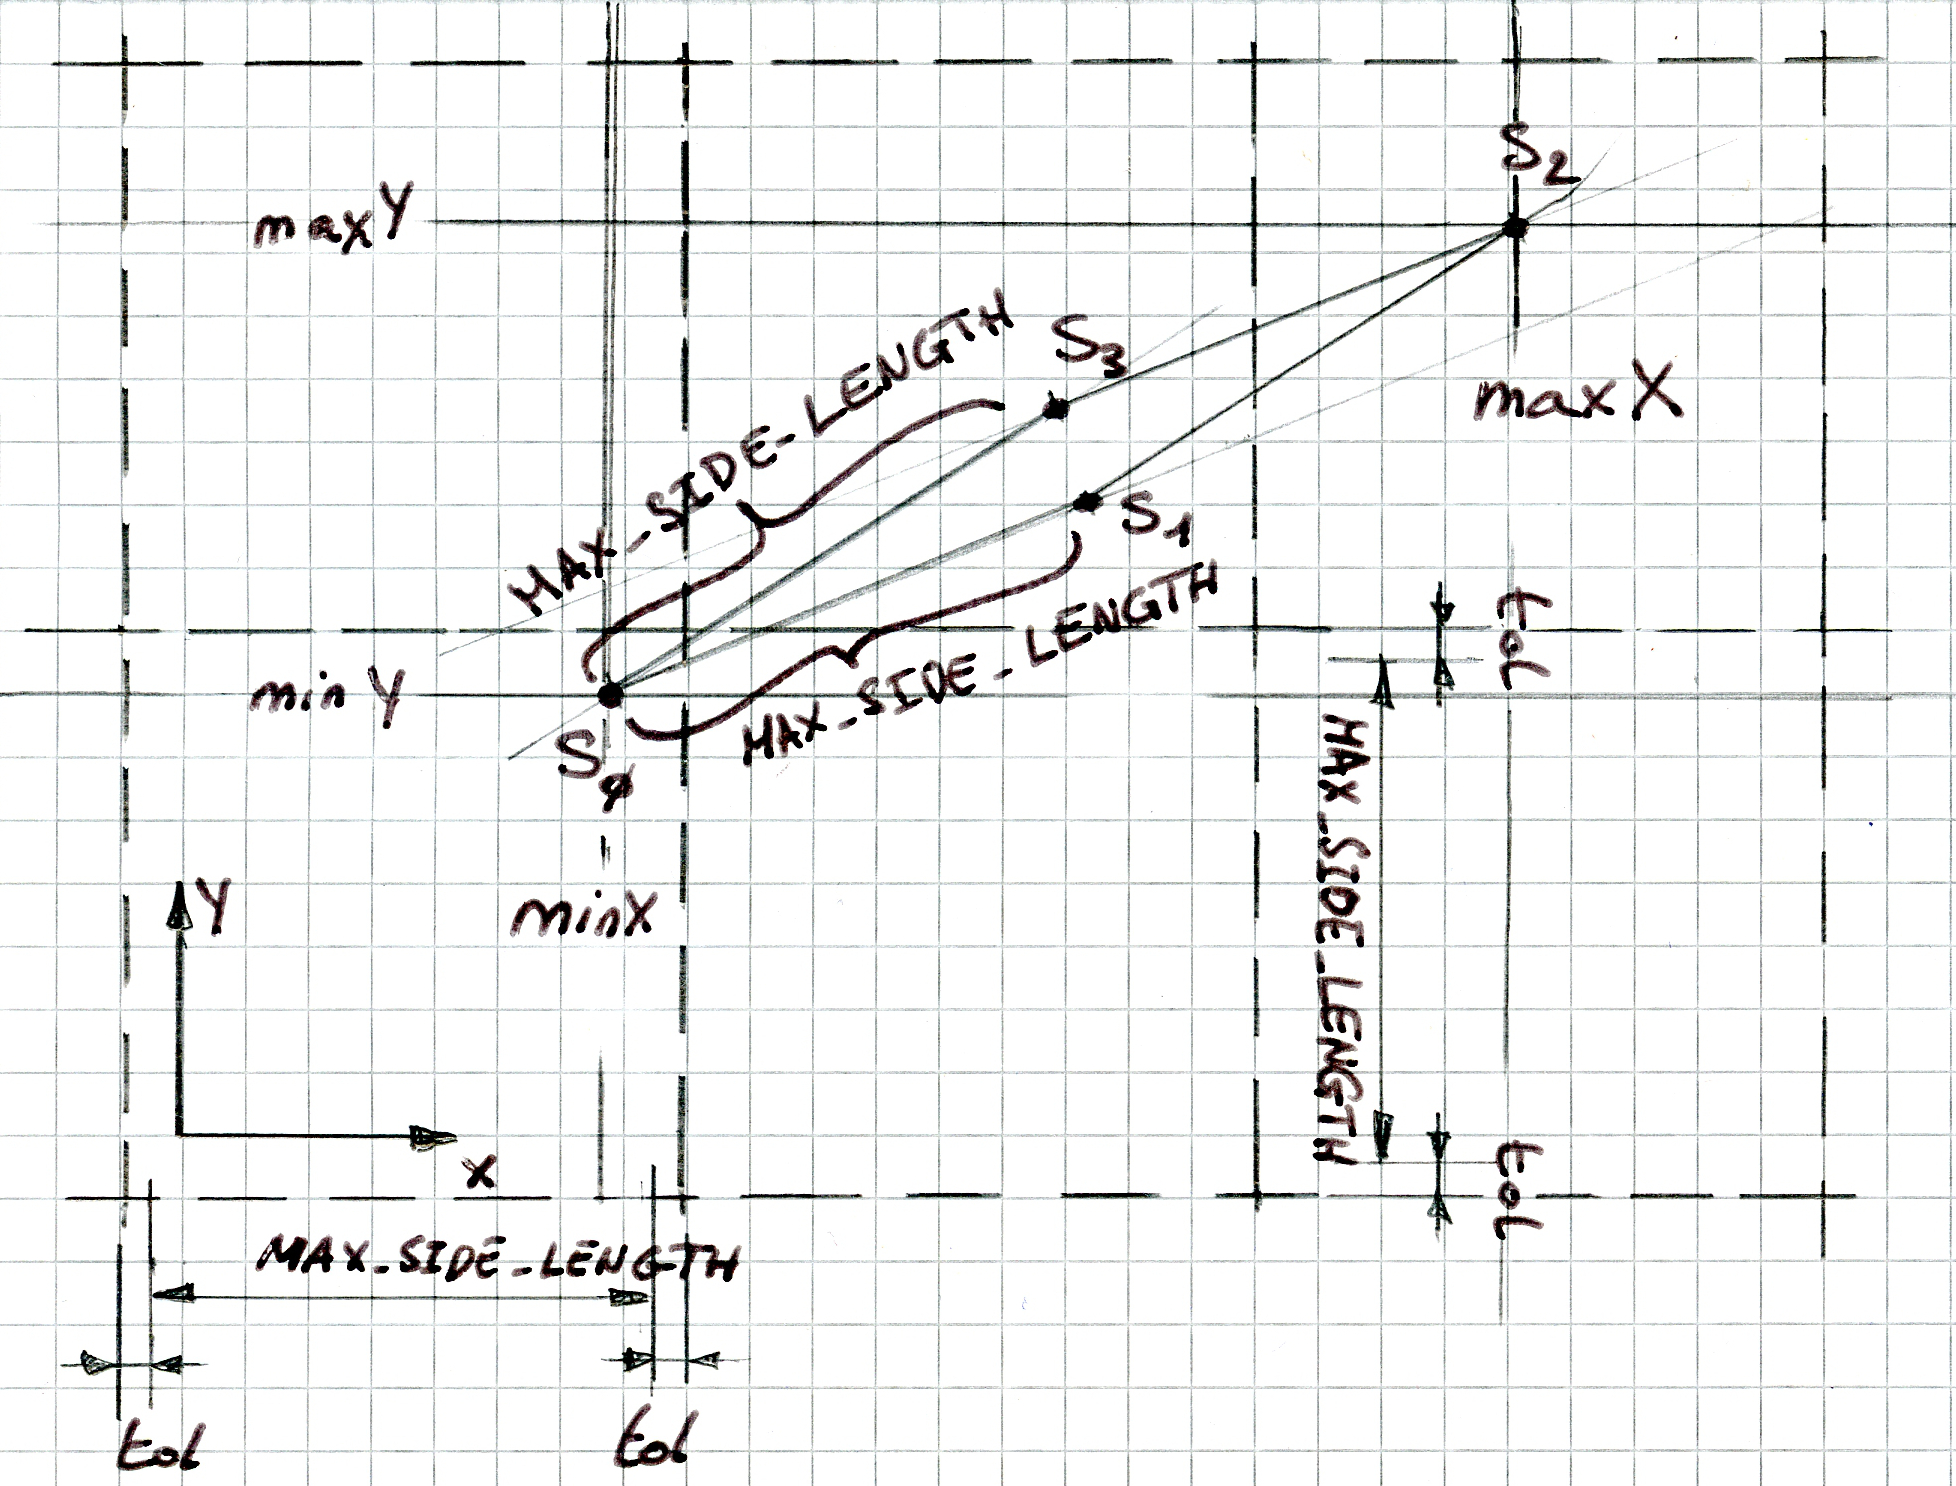
\includegraphics[width=0.5\linewidth]{includes/images/quadri1}
 \caption{Placement d'un QCar dans le quadrillage}
 \label{fig:quadri1}
\end{figure}
Afin de ne pas avoir de ${NuUllPointerException} $ sur le tableau quadrillage, la taille de base d'un côté du tableau sera de la taille d'un côté de l'espace occupé par un QCar sur ce tableau multipliée par une fois et demie, le tout multiplié par le nombre de QCar ${nbrQCar}$ présent sur l'aire de jeu, toutes natures confondues, ceci étant la taille nécessaire pour faire tenir tous les QCars sur une seule ligne du quadrillage. Cette valeur sera référée comme étant la dispersion maximale $ {maxDispersion}$ des coordonnées des QCars sur l'une des ordonnées de l'aire de jeu.
\[ {maxDispersion} = ((2 * MAX\_SIDE\_LENGTH + 4 * tol) * 1.5) * nbrQCar \]
\subsubsection{Calcul des coordonnées}
\paragraph{Sommet 0}Le calcul des coordonnées commence par un choix de coordonnées de valeurs aléatoires pour le sommet $S_{0}$ numéro zéro du QCar, qui sera défini comme une ancre sur l'aire de jeu, tous les autres sommets étant choisis par rapport à cette première position. Les coordonnées $ X_{S_{0}} $ et $ Y_{S_{0}} $ de ce sommet sont choisies de telle manière à ce qu'elles remplissent la condition $0,0 < X_{S_{0}} \le maxDispersion $ et $0,0 < Y_{S_{0}} \le maxDispersion $.
\paragraph{Côté 1: base du parallélogramme}La base $\mathit{side1}$ du parallélogramme QCar est obtenue aléatoirement de telle manière à ce qu’ $0,0 < \mathit{side1} \le MAX\_SIDE\_LENGTH $ afin d'éviter d'obtenir des segments de droites.
La hauteur minimale $minH$ du parallélogramme QCar nécessaire pour respecter l'aire minimale $minArea$ spécifiée dans la nature du QCar est calculée avec la formule suivante:
\[ minH = \frac{minArea}{\mathit{side1}} \]
avec la contrainte $0,0 < minH \le MAX\_SIDE\_LENGTH $. 
La base $\mathit{side1}$ et la hauteur minimale $minH$ seront recalculées jusqu'à ce que $minH$ respectent les contraintes.
\begin{figure}[h!]
 \centering
 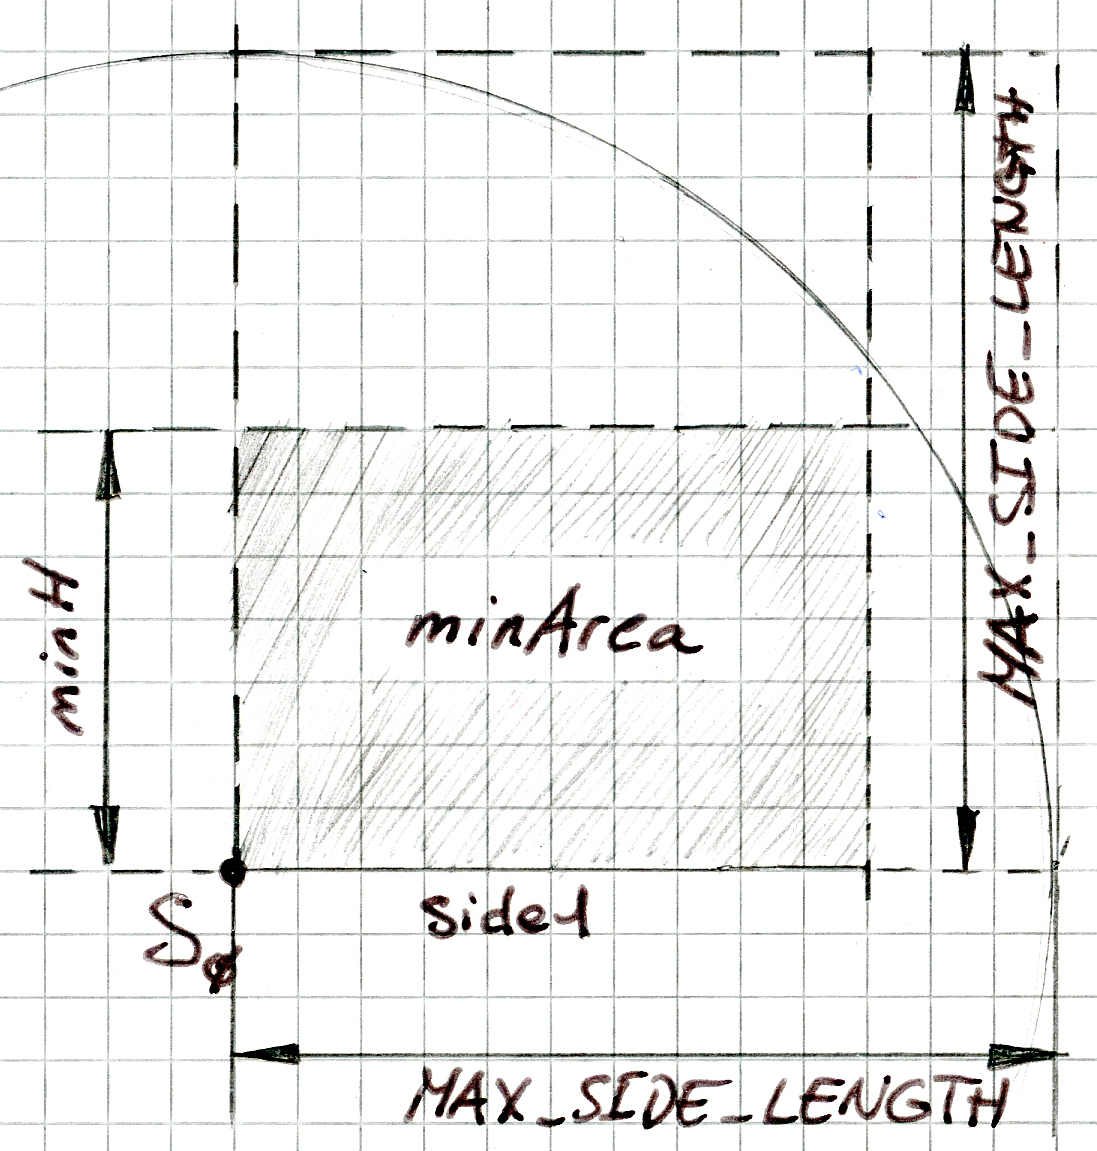
\includegraphics[width=0.4\linewidth]{includes/images/creaQCar1}
 \caption{Calcul de minH}
 \label{fig:creaqcar1}
\end{figure}
\paragraph{Côté 2}
Le côté numéro deux $\mathit{side2}$ du parallélogramme est récupéré en obtenant aléatoirement sa portée contenue dans l'intervalle $[minH;MAX\_SIDE\_LENGTH]$ en suivant la formule:
\[\mathit{side2} = minH + val * \left|MAX\_SIDE\_LENGTH-minH\right|   \] 
avec $val$ une valeur aléatoire respectant la contrainte $ 0,0 \le val < 1,0$.
\begin{figure}[h!]
 \centering
 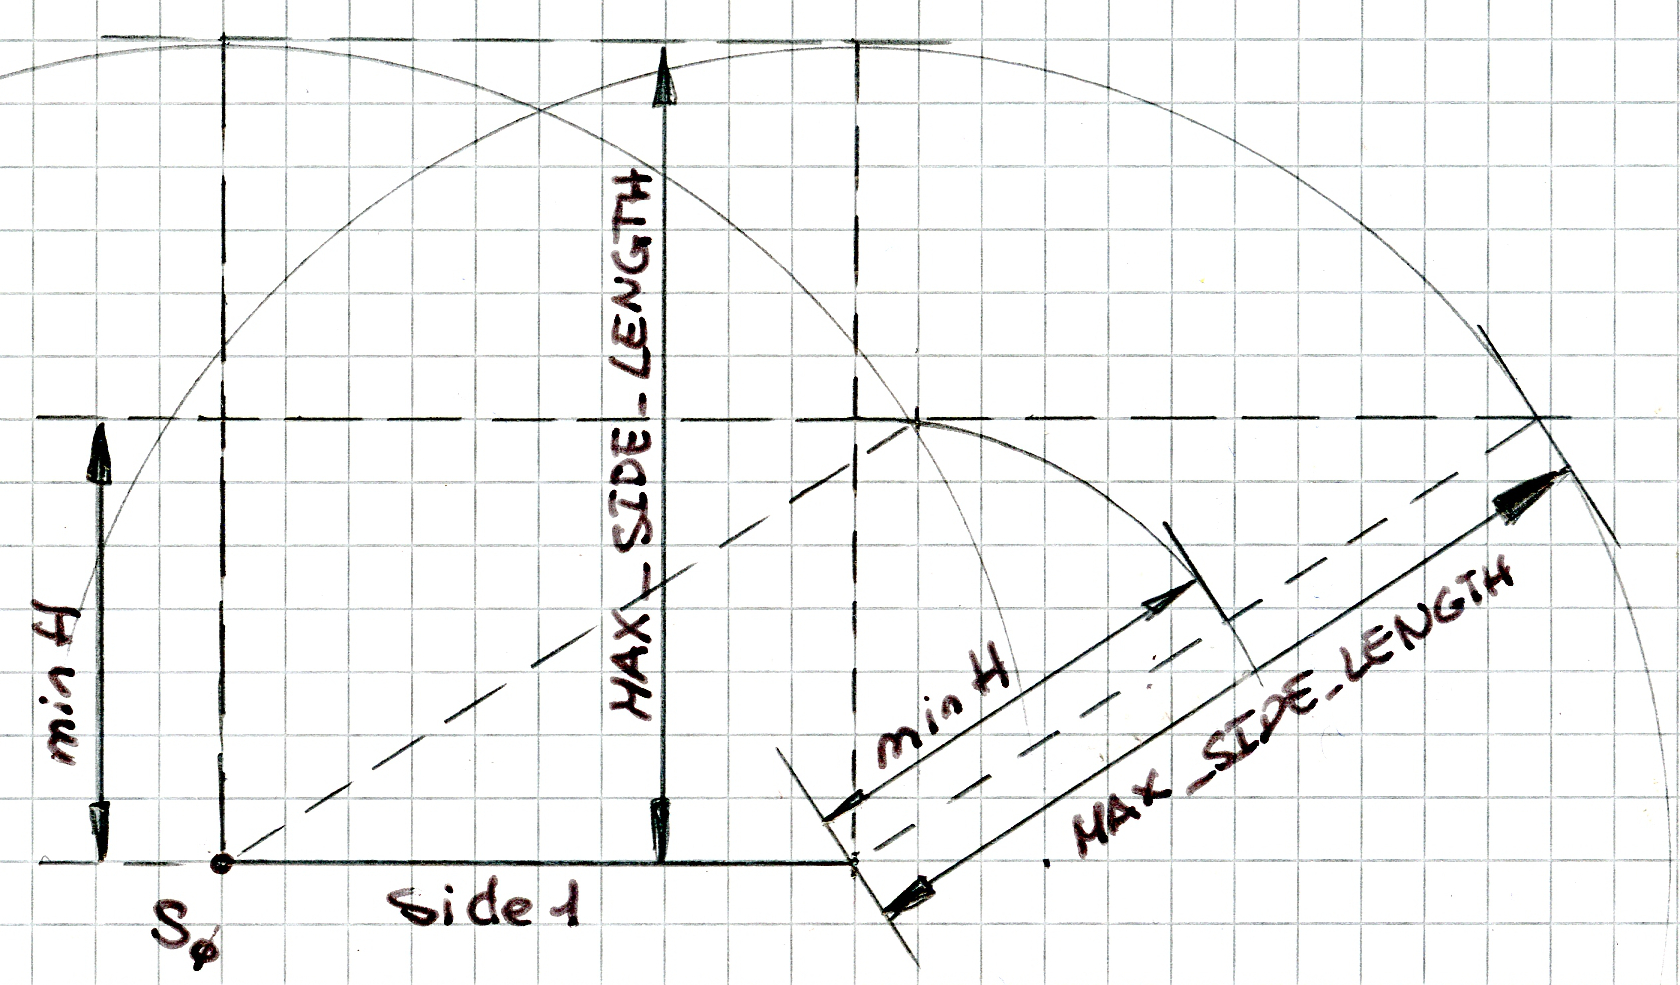
\includegraphics[width=0.6\linewidth]{includes/images/creaQCar2}
 \caption{Portée de side2}
 \label{fig:creaqcar2}
\end{figure}
\paragraph{Calcul de l'offset et de la hauteur effective}
On calcule en premier l'offset maximal $maxOffset$ qui permet de respecter la contrainte $minArea$ en utilisant le théorème de Pythagore:
\[ maxOffset =\sqrt{\left|\mathit{side2}^{2}-minH^{2}\right|} \]
\begin{figure}[h!]
 \centering
 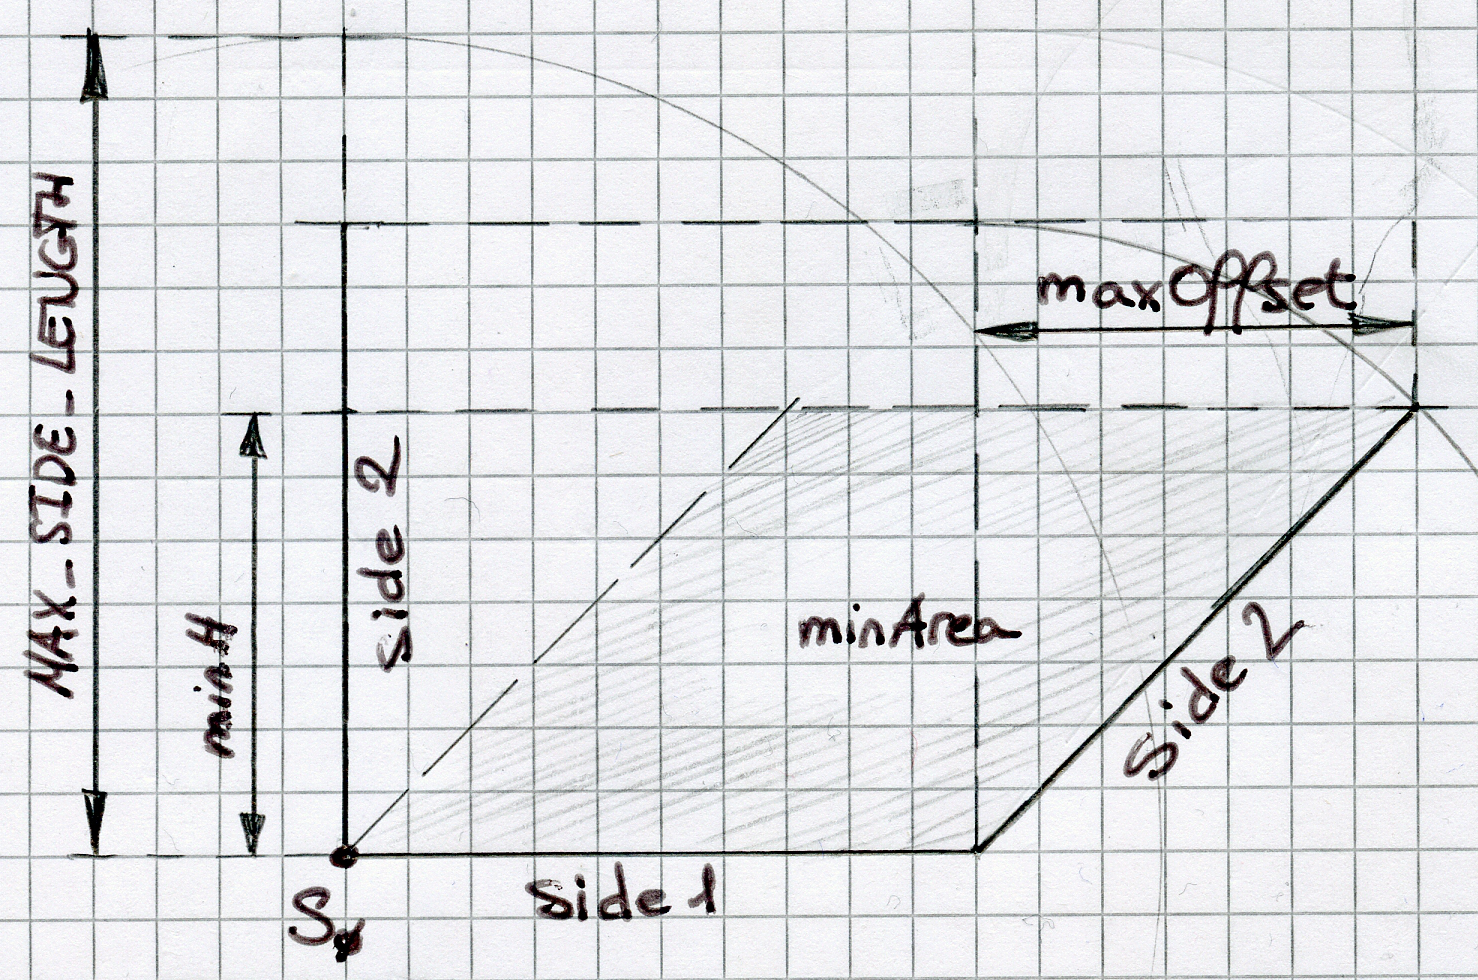
\includegraphics[width=0.5\linewidth]{includes/images/creaQCar3}
 \caption{Portée maximale de l'offset}
 \label{fig:creaqcar3}
\end{figure}
On peut ensuite tirer une valeur d'offset $offset$ aléatoire comprise dans l'intervalle $[0,0;maxOffset]$ et l'utiliser pour calculer la hauteur $H$ effective du parallélogramme QCar en appliquant à nouveau Pythagore:
\[ H =\sqrt{\left|\mathit{side2}^{2}-offset^{2}\right|} \]
Les valeurs $\mathit{side1}$, $\mathit{side2}$ et $H$ ainsi obtenues vont nous permettre d'obtenir les coordonnées correctes des sommets $S_{1}, S_{2}$ et $S_{3}$ du QCar.
\begin{figure}[h!]
 \centering
 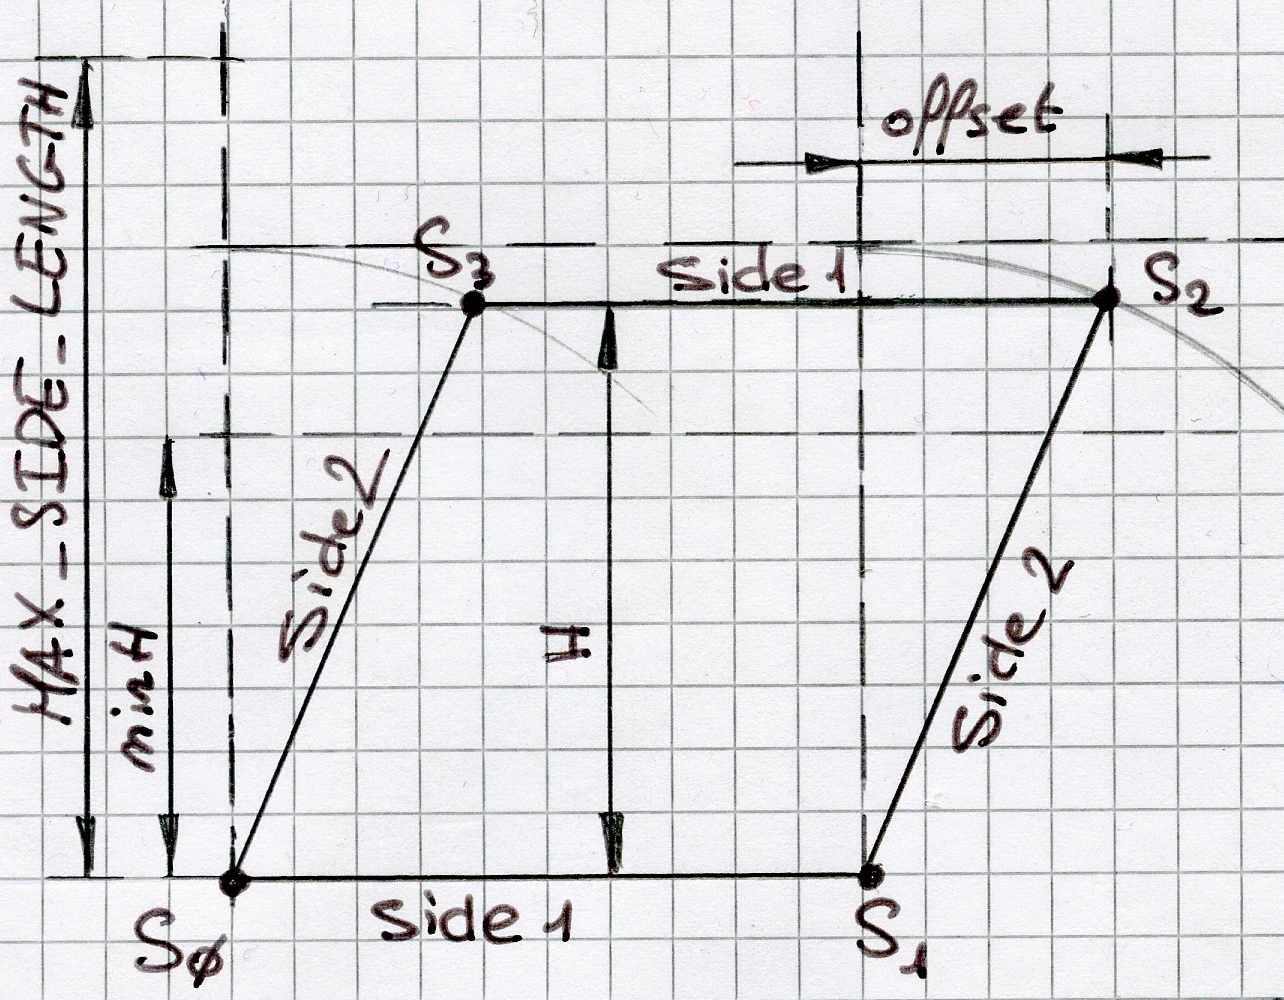
\includegraphics[width=0.4\linewidth]{includes/images/creaQCar4}
 \caption{Les valeurs $\mathit{side1}$, $\mathit{side2}$ et $H$ finales}
 \label{fig:creaqcar4}
\end{figure}
\paragraph{Calcul des coordonnées de $S_{1}, S_{2}$ et $S_{3}$}
Pour les coordonnées de $S_{1}, S_{2}$ et $S_{3}$, il y a quatre cas de figure possibles:
\begin{itemize}
\item l'offset est orienté horizontalement et se dirige vers la droite
\item l'offset est orienté horizontalement et se dirige vers la gauche
\item l'offset est orienté verticalement et se dirige vers le haut
\item l'offset est orienté verticalement et se dirige vers le bas
\end{itemize}
\begin{figure}[h!]
 \centering
 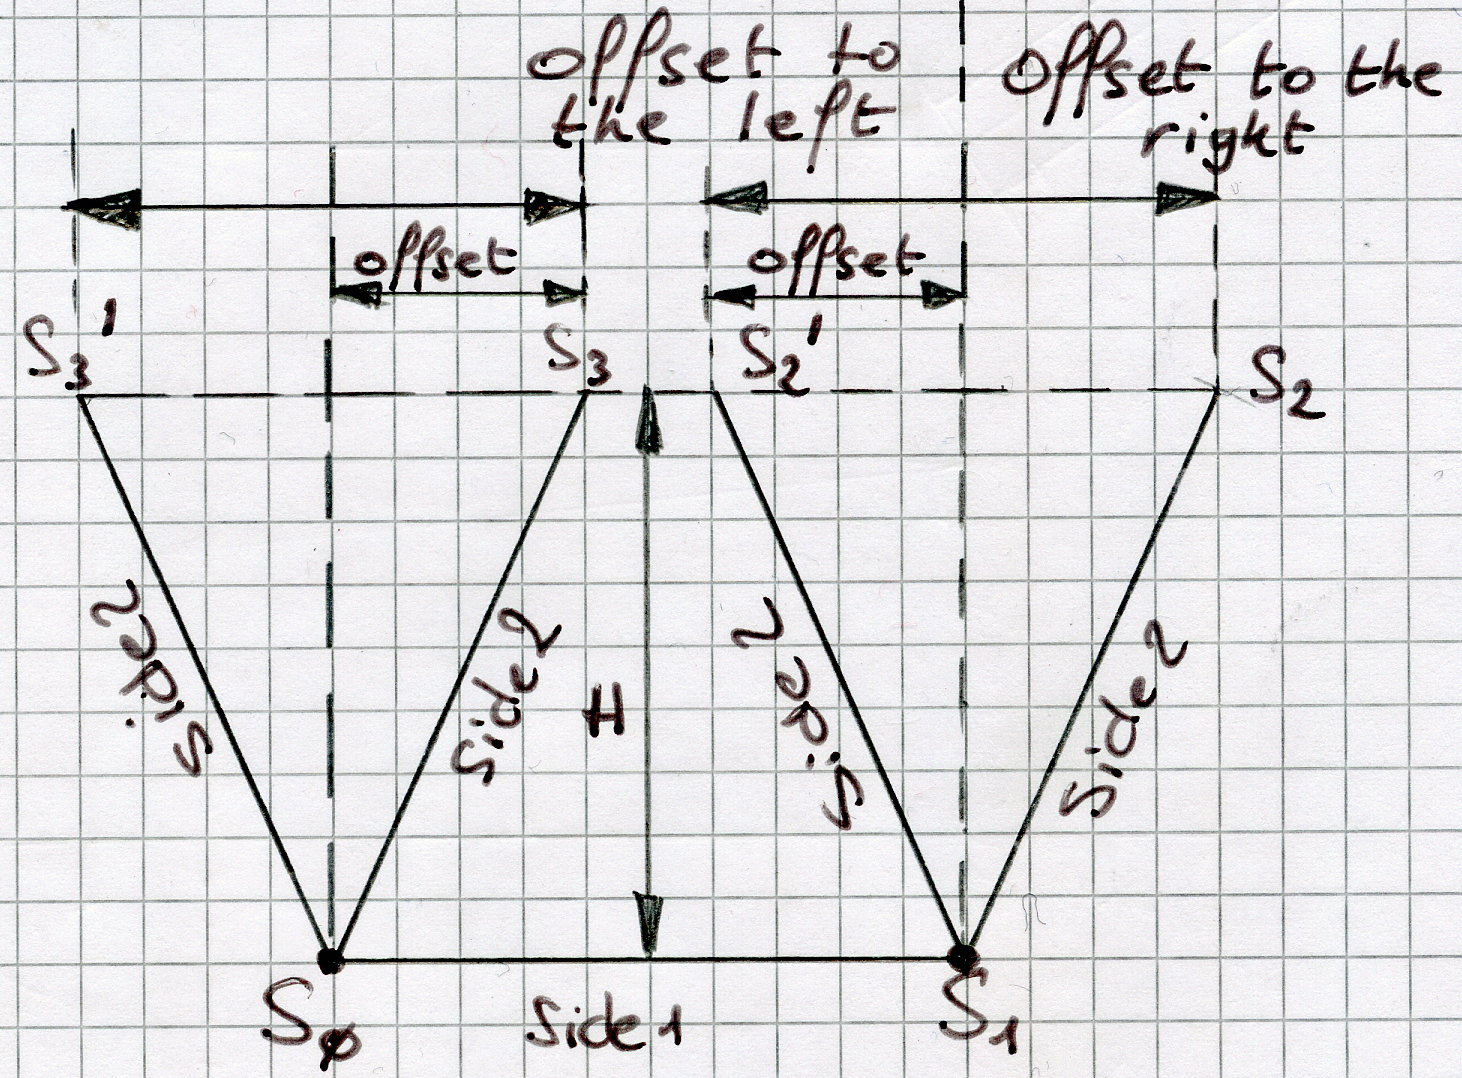
\includegraphics[width=0.3\linewidth]{includes/images/creaQCar5offsethoriz}
 \caption{Offset horizontal}
 \label{fig:creaqcar5offsethoriz}
\end{figure}
\begin{figure}[h!]
 \centering
 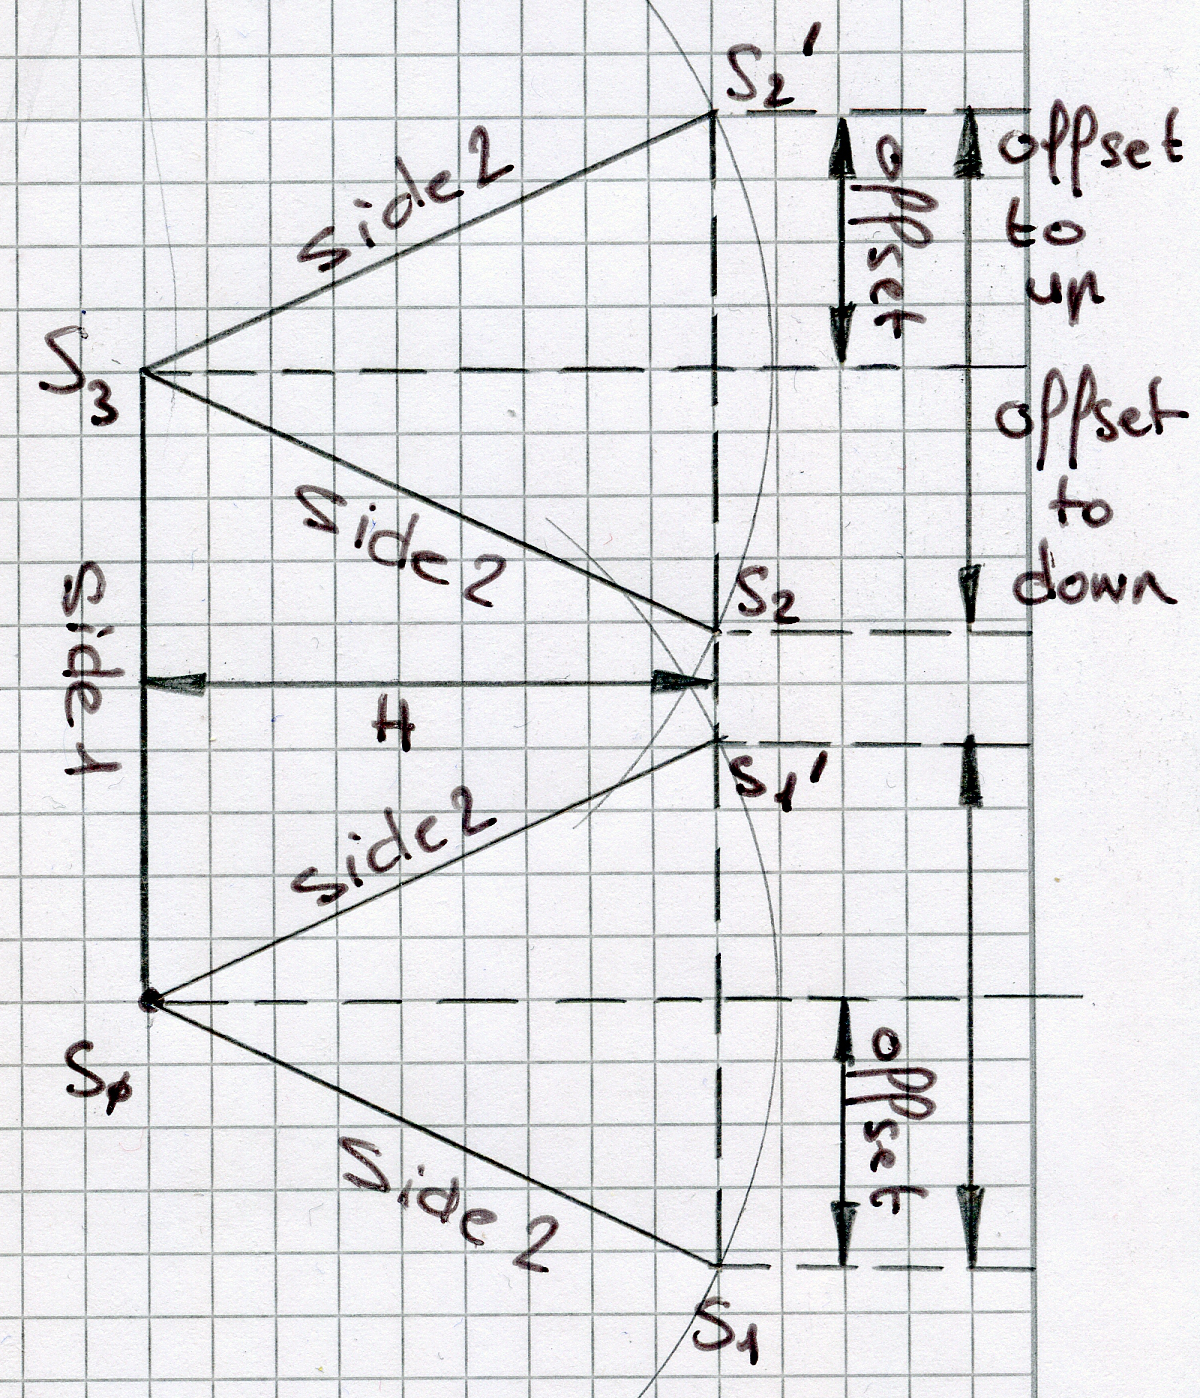
\includegraphics[width=0.3\linewidth]{includes/images/creaQCar6offsetverti}
 \caption{Offset vertical}
 \label{fig:creaqcar6offsetverti}
\end{figure}
Ces cas de figure sont choisis aléatoirement et les coordonnées sont calculées en fonction du sommet ancre $S_{0}$ avec les valeurs de $\mathit{side1}$, $H$ et $offset$. On vérifie les coordonnées en X et Y pour qu'elles soient bien supérieures ou égales à zéro. Si les coordonnées en X sont négatives, on ajoute la valeur absolue de l'offset sur les valeurs en X de tous les sommets et réciproquement pour les coordonnées en Y. 
\paragraph{Rotation de la figure}
La dernière transformation effectuée sur le parallélogramme est une rotation aléatoire avec un angle compris dans l'intervalle $[0,0; 2\Pi]$ radiant sur son centre de symétrie.
\paragraph{Vérification du placement}
La dernière étape est la validation du placement du QCar sur l'aire de jeu en prenant la coordonnée X minimale $minX$ de tous ses sommets, celle minimale en Y $minY$, celle maximale en X $maxX$ et maximale en Y $maxY$ en vérifiant l'occupation du tableau du quadrillage sur le sous-quadrillage:
\[\begin{array}{ccc}
 minX,maxY & ... & maxX,maxY \\ 
 ... & ... & ... \\ 
 minX,minY & ... & maxX,minY
\end{array}\]
Si le sous-quadrillage est libre, le QCar se réserve l'emplacement, sinon, la procédure de création est reprise depuis le début.
\subsubsection{Génération des styles}
La génération des QCars de nature "driven" est toujours effectuée en premier et ils sont placé au début de la liste de QCars. Les natures secondaires "static" et "parking" sont ensuite générées avec un choix de nature aléatoire en fonction du style choisi. Tous les QCars verront leurs coordonnées générées et vérifiées en utilisant la méthode décrite ci-dessus.
\subsection{PhysicsHelper}
\subsubsection{Collisions}
Le QCar piloté est celui avec l'ID 0. Deux cas vont être traités dans les exemples suivants : un mouvement linéaire (non angulaire) et un mouvement angulaire. Dans le premier cas, le QCar 0 désire déplacer son côté \no2 positivement. La longueur du déplacement correspond à la longueur du côté \no3. Dans le deuxième cas, le QCar 0 désire déplacer son côté \no 2 négativement. La longueur du déplacement correspond à la longueur du côté \no2.
\begin{figure}[h!]
\centering
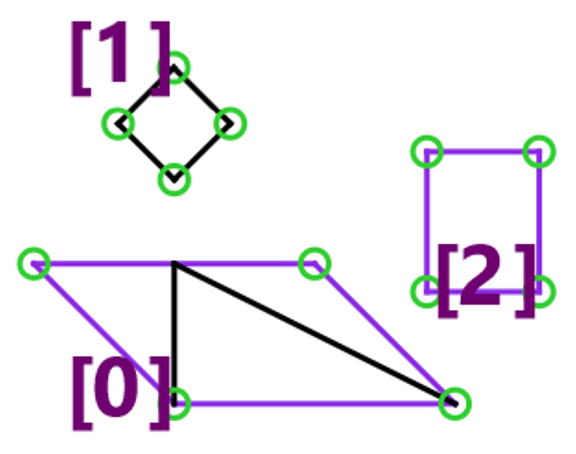
\includegraphics[width=0.4\linewidth]{includes/images/collisions/1_initialState}
\caption{Exemple collision : état initial}
\label{fig:1initialstate}
\end{figure}
Pour détecter si une collision aura lieu ou non, il faut observer et analyser l'aire balayée (zone traitillée rouge) par le déplacement du côté utilisé.
\begin{figure}[h!]
\centering
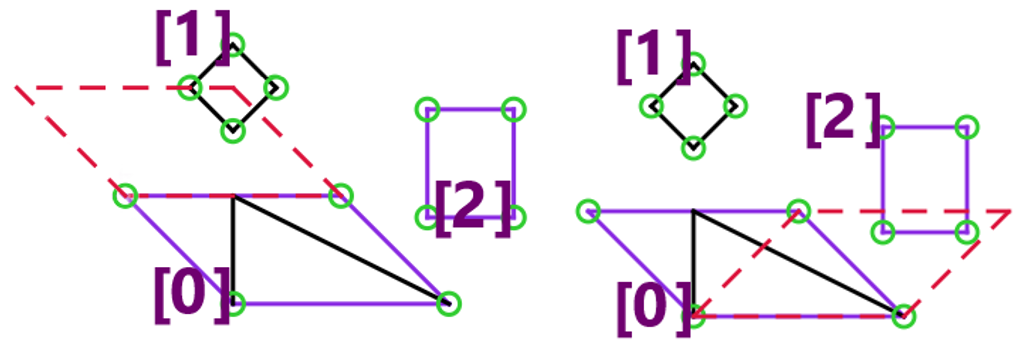
\includegraphics[width=0.7\linewidth]{includes/images/collisions/2_sweptArea}
\caption{Exemple collision : visualisation de l'aire balayée}
\label{fig:2sweptarea}
\end{figure}
Il va donc falloir vérifier en premier lieu si un vertex de n'importe quel Qcar se trouve dans la zone balayée ou sur ses limites. Pour cela, un nouveau système d'axes sera généré par rapport au Qcar et au déplacement. Si on veut déplacer le QCar avec un mouvement non angulaire, l'axe $\vec{a1}$ doit se placer exactement sur le côté à déplacer et sa norme correspond à la longueur du côté. L'axe $\vec{a2}$ doit se placer parallèlement au côté dont l'ID est celui du côté déplacé augmenté de un. Si la longueur de mouvement est négative, alors aucune nouvelle collision n'est à prévoir. Si on veut déplacer le QCar avec un mouvement angulaire, l'axe $\vec{a1}$ doit se placer parallèlement au côté dont l'ID est celui du côté déplacé augmenté/diminué de un selon le signe de déplacement. L'axe $\vec{a1}$ doit se placer exactement sur le côté à déplacer et sa norme correspond à la longueur du côté. L'origine des deux axes est donc déterminée selon le signe du déplacement.
\begin{figure}[h!]
\centering
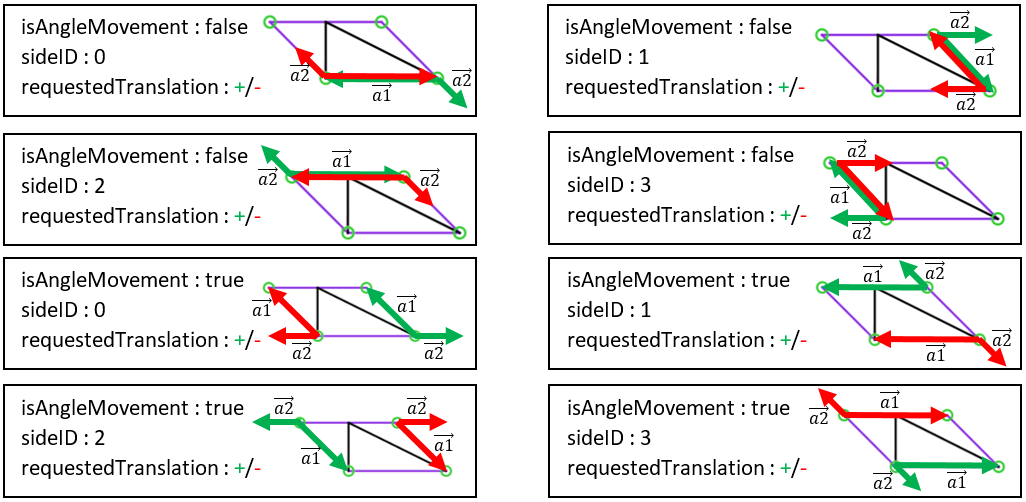
\includegraphics[width=\linewidth]{includes/images/collisions/3_axes}
\caption{Exemple collision : différents placements des axes $\vec{a1}$ et $\vec{a2}$}
\label{fig:3axes}
\end{figure}
Tous les sommets de tous les QCars inclus dans la simulation (lui-même exclu) sont transformés par une matrice de passage. Les résultats de cette transformation sont donc des points avec leurs coordonnées exprimées dans la base $\vec{a1}$ $\vec{a2} $ (A). Pour tester si un point se trouve dans la zone "critique" à la suite d'une décision impliquant un mouvement linéaire (non angulaire), il suffit de tester si ses coordonnées $\vec{a1}$ et $\vec{a2}$ sont inclues entre 0 et 1 compris. Si la coordonnée $\vec{a2}$ vaut zéro, cela signifie que la collision a déjà été détectée au dernier pas de simulation. A l'inverse, pour un mouvement angulaire, il faut également tester les conditions semblables au mouvement linéaire. Mais en plus, il faut tester que la condition du rapport (coordonnée $\vec{a2}$/(1 - coordonnée $\vec{a1}$) soit plus petite ou égale à, $||\vec{a2}||/||\vec{a1}||$ car l'aire balayée est un triangle et non un rectangle. Cette condition se base sur des triangles semblables.
\begin{figure}[h!]
\centering
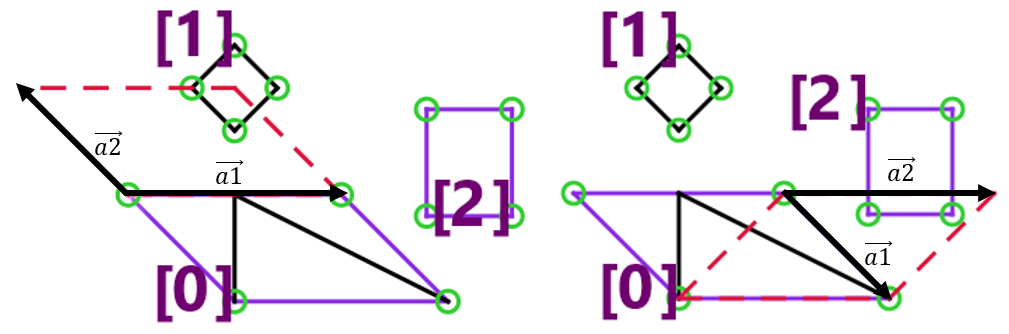
\includegraphics[width=0.7\linewidth]{includes/images/collisions/4_axesPosition}
\caption{Exemple collision : placement des axes $\vec{a1}$ et $\vec{a2}$ + région balayée}
\label{fig:4axesposition}
\end{figure}
Lorsque l'on a détecté qu'un point se trouve dans la région balayée par le mouvement, il faut définir si cette éventuelle collision sera la finale. Pour effectuer cette tâche, la coordonnée  $\vec{a2}$ est indispensable. Dans le cas d'un mouvement linéaire, cette coordonnée suffit. Le point de la collision finale aura la coordonnée $\vec{a2}$ la plus petite. Dans le cas d'un mouvement angulaire, c'est le rapport (coordonnée $\vec{a2}$)/(1 - coordonnée $\vec{a1}$) le plus petit qui va faire foi.
Voici les points potentiellement intéressants qui sont trouvés dans la zone "critique". Pour l'instant, les collisions seront engendrées avec les points bleus à la bordure rouge. Ce sont ces points qui ont soit la coordonnée $\vec{a2}$ la plus petite soit le rapport (coordonnée $\vec{a2}$)/(1 - coordonnée $\vec{a1}$) le plus petit.
\begin{figure}[h!]
\centering
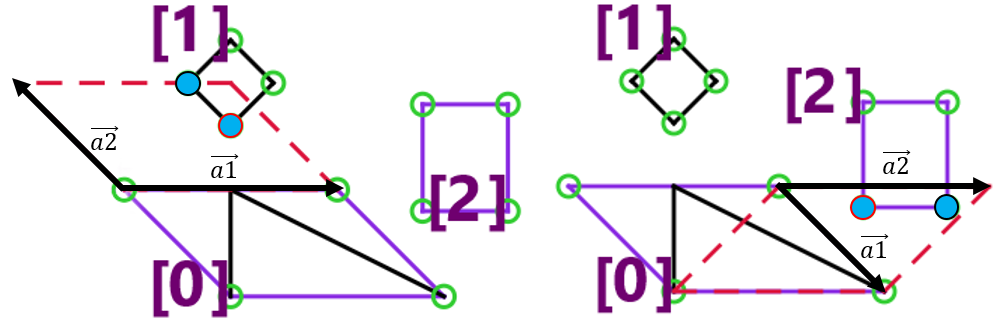
\includegraphics[width=0.7\linewidth]{includes/images/collisions/5_pointCheck}
\caption{Exemple collision : test des points dans la zone}
\label{fig:5pointcheck}
\end{figure}
Une fois le test du point effectué, le côté se situant à la droite du point testé est analysé. Pour cela, on a besoin d'une droite passant par les deux points constituant le segment et des droites qui définissent la zone "critique". En cas de mouvement angulaire, deux droites délimitent la zone, sinon trois (en rouge). Les droites des côtés sont en bleu. 
\begin{figure}[h!]
\centering
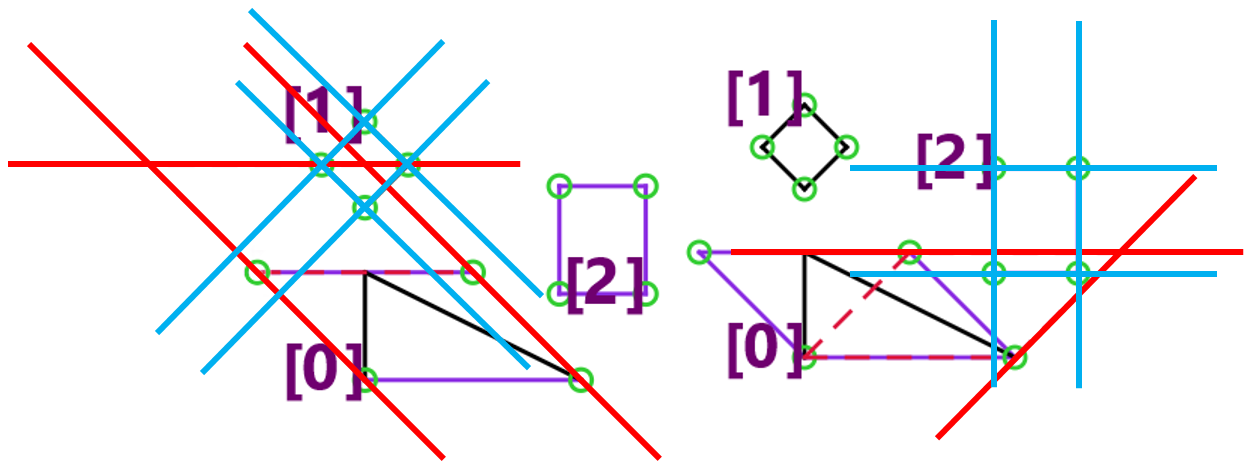
\includegraphics[width=0.7\linewidth]{includes/images/collisions/6_lines}
\caption{Exemple collision : droites}
\label{fig:6lines}
\end{figure}
Les collisions potentielles sont les points d'intersection. Une fois ceux-ci trouvés, il faut vérifier que ces points d'intersection sont sur les segments et non uniquement sur les droites.
\begin{figure}[h!]
\centering
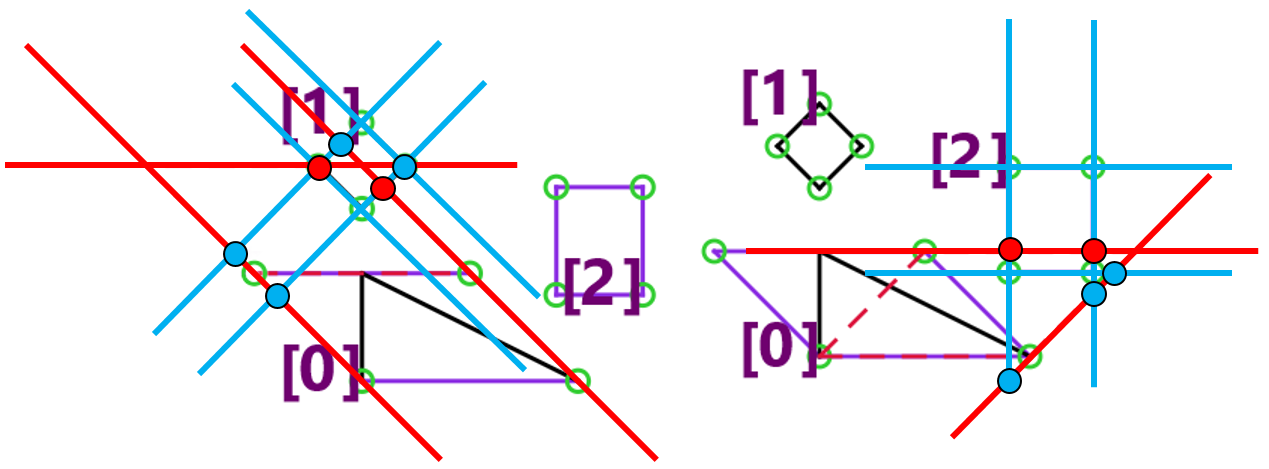
\includegraphics[width=0.7\linewidth]{includes/images/collisions/7_linesIntersections}
\caption{Exemple collision : intersection des droites, collisions potentielles}
\label{fig:7linesintersections}
\end{figure}
Les points bleus sur les illustrations ci-dessus n'ont pas passé le test précédent donc ils sont ignorés. Par contre, les points rouges sont transformés par la matrice de passage. Si leur coordonnée $\vec{a2}$ est plus petite que la coordonnée $\vec{a2}$ de la collision actuelle (si elle existe), alors le point devient la collision actuelle.
Finalement, pour le premier exemple, une collision est détectée entre le QCar 0 et le QCar 1. Dans le deuxième exemple, une collision est détectée entre le QCar 0 et le QCar 2.
\begin{figure}[h!]
\centering
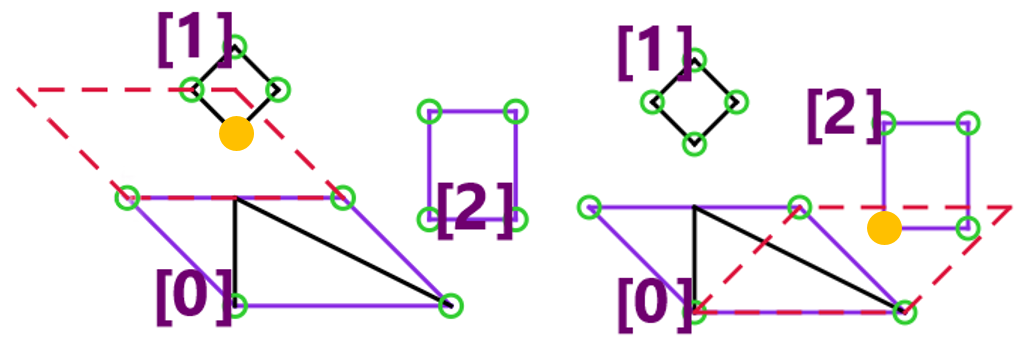
\includegraphics[width=0.7\linewidth]{includes/images/collisions/8_collisionPoints}
\caption{Exemple collision : points de collision détectés}
\label{fig:8collisionpoints}
\end{figure}
Une fois toutes les collisions correctes détectées, on aimerait déplacer le QCar selon la décision demandée jusqu'à la collision et pas plus loin. Pour faire ceci, on calcule le point de la collision projeté sur l'axe $\vec{a2}$ (points rouges sur les graphiques ci-dessous). Et comme l'axe $\vec{a2}$ est toujours le vecteur dirigé dans le sens du déplacement, on sait de combien il va falloir déplacer les points formant le côté à bouger du QCar.
\begin{figure}[h!]
\centering
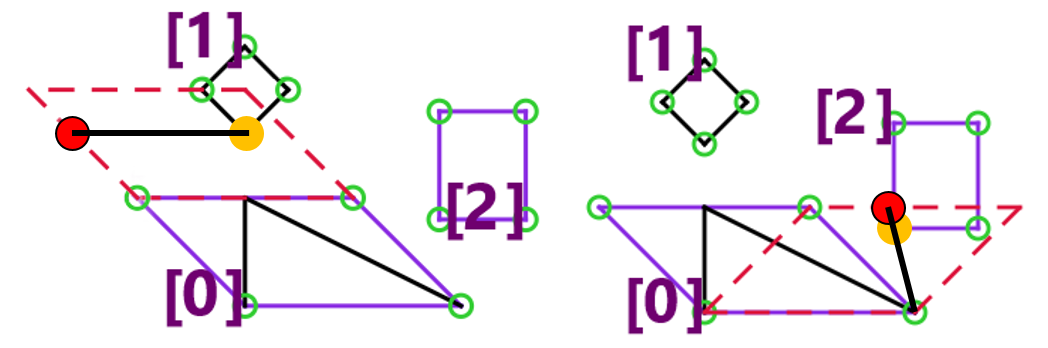
\includegraphics[width=0.7\linewidth]{includes/images/collisions/9_projectionPoints}
\caption{Exemple collision : projection des points}
\label{fig:9projectionpoints}
\end{figure}
On applique ensuite aux points du côté à bouger la translation du vecteur avec pour fin de flèche le point projeté et pour origine l'origine des axes $\vec{a1}$ et $\vec{a2}$, exprimée en x et y.
On obtient finalement ces situations suivant le mouvement.
\begin{figure}[h!]
\centering
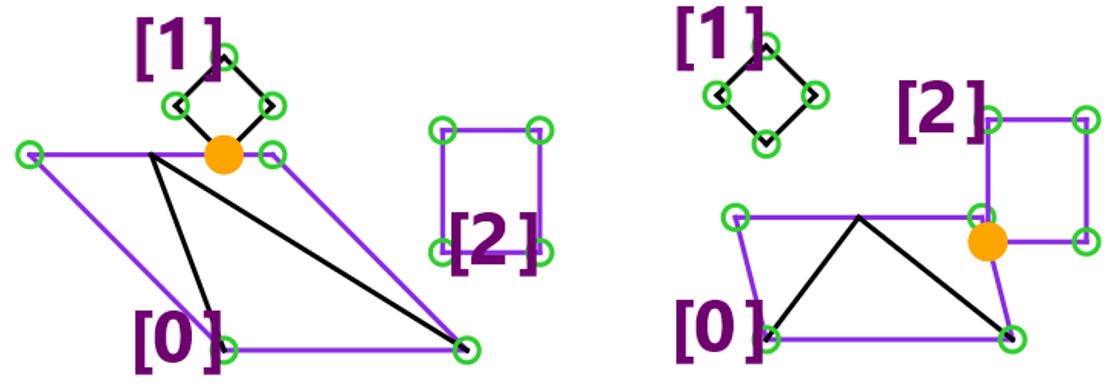
\includegraphics[width=0.7\linewidth]{includes/images/collisions/10_finalState}
\caption{Exemple collisions : état final}
\label{fig:10finalstate}
\end{figure}
\subsubsection{Sensors}
Concernant le calcul des sensors, on a regroupé deux traitements en un seul. Les calculs des SeenVertices et du DistanceSensor sont effectués dans la même méthode.
Le système utilisé est semblable à celui de l'algorithme de détection de collisions. On va donc également utiliser les axes $\vec{a1}$ et $\vec{a2}$ ainsi qu' une matrice de passage pour convertir les points d'une base à l'autre (essentiellement XY vers A).
Le situation initiale est présentée sur la figure \ref{fig:1initialstatesensors}.
\begin{figure}[H]
\centering
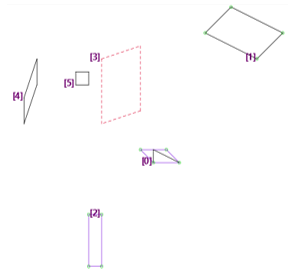
\includegraphics[width=0.5\linewidth]{includes/images/sensors/1_initialState}
\caption{Sensors : état initial}
\label{fig:1initialstatesensors}
\end{figure}
Les axes $\vec{a1}$ et $\vec{a2}$ sont placés sur le côté \no 2 du QCar avec pour origine l'œil. La zone visible est définie par les deux axes. Elle est "accédée" par l'œil (eye) qui se trouve au milieu du côté \no 2 du QCar. Si l'aire de simulation est bornée par un QCar "externe", alors la zone visible est également bornée telle que la deuxième illustration le démontre. Dans le cas contraire, la vision est infinie. 
\begin{figure}[H]
\centering
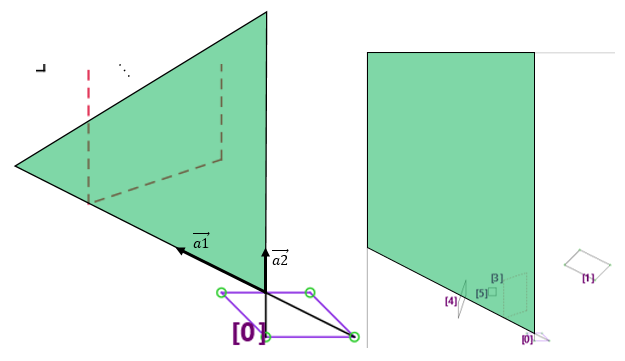
\includegraphics[width=0.7\linewidth]{includes/images/sensors/2_seenAreas}
\caption{Sensors : aires balayées}
\label{fig:2seenareas}
\end{figure}
Une fois les axes de vision définis, il va falloir tester chaque vertex de chaque QCar. Pour appliquer ceci, on transforme le point concerné à l'aide de la matrice de passage. Les coordonnées du point en sortie sont exprimées en base A. L'unique condition à vérifier pour que ce point soit potentiellement visible par le QCar est que ses nouvelles coordonnées soient positives ou égales à zéro.
Les points rouges sont les points non visibles et les verts sont les points potentiellement visibles.
\begin{figure}[H]
\centering
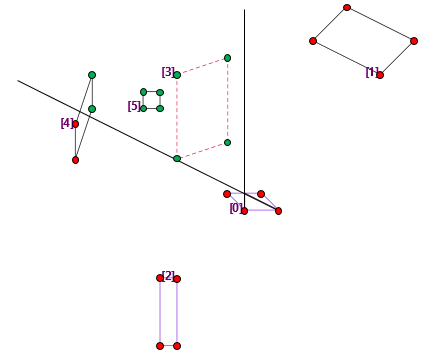
\includegraphics[width=0.7\linewidth]{includes/images/sensors/3_pointsInclusion}
\caption{Sensors : point inclus}
\label{fig:3pointsinclusion}
\end{figure}
Maintenant, la condition pour qu'un point potentiellement visible devienne non-visible est qu'un côté de QCar (surtout un des siens) ait une intersection avec le segment "point potentiellement visible" – œil (eye).
Dans le cas du QCar n° 5, on remarque que le segment "point rouge" – œil est intersecté par les deux segments bleus (côtés du même QCar). Le point rouge devient donc invisible.
\begin{figure}[H]
\centering
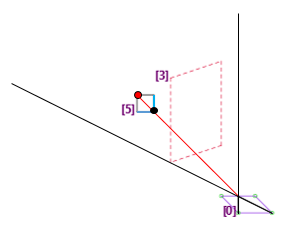
\includegraphics[width=0.5\linewidth]{includes/images/sensors/4_nonIncludedPoint}
\caption{Sensors : point non inclus}
\label{fig:4nonincludedpoint}
\end{figure}
Si le point est bien visible, il faut calculer la projection du segment point – œil. C'est le point projeté sur le côté \no 0 du QCar. Il est utilisé dans le constructeur du SeenVertex. Pour cela, la méthode de recherche d'intersection est très utile. On va chercher "l'intersection" entre la droite point – œil et le côté \no 0 du QCar.
\begin{figure}[H]
\centering
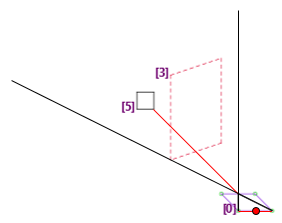
\includegraphics[width=0.5\linewidth]{includes/images/sensors/5_projectedPoint}
\caption{Sensors : point projeté}
\label{fig:5projectedpoint}
\end{figure}
En ce qui concerne le DistanceSensor, pour chaque point testé, on vérifie le segment se trouvant à sa droite. On cherche "l'intersection" entre ce segment et le segment "milieu du côté \no 1 du QCar" – œil. Le point d'intersection du DistanceSensor final aura la coordonnée $\vec{a2}$ la plus petite. Dans l'illustration ci-dessous, il y aura deux intersections avec la même coordonnée $\vec{a2}$. C'est la première intersection qui va être retenue.
\begin{figure}[H]
\centering
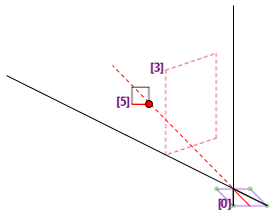
\includegraphics[width=0.5\linewidth]{includes/images/sensors/6_distanceSensor}
\caption{Sensors : Illustration du DistanceSensor}
\label{fig:6distancesensor}
\end{figure}
Ainsi on peut voir ce que voit le QCar sur la figure \ref{fig:7seenvertices}
\begin{figure}[H]
\centering
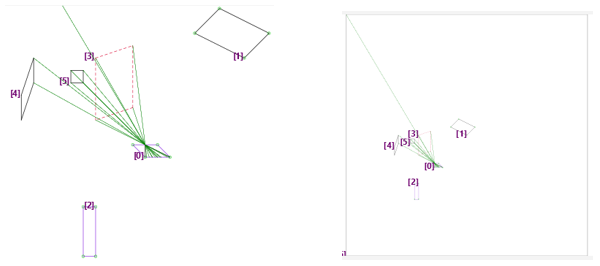
\includegraphics[width=\linewidth]{includes/images/sensors/7_seenVertices}
\caption{Sensors : résultat de SeenVertices}
\label{fig:7seenvertices}
\end{figure}

\subsection{WorldManager}
Le WorldManager utilise en grande partie les fonctionnalités implémentées dans WorldManagerPhysicsHelper. 
\paragraph{openNewSimulation} 
Cette méthode initialise toutes les variables nécessaires à une partie, elle récupère une liste de QCars, initialise un sémaphore chargé de synchroniser les pas de simulation (dans le cas où tous les pilotes ont donné leur décision avant la fin du temps imparti). Les PlayersChannels sont créés à partir de la liste des Sensors et sont fournis aux Drivers lorsqu'on lance les threads des drivers.
\paragraph{simulateOneStep}
Le but de la méthode est, comme son nom l'indique, de lancer un pas de simulation, en récupérant les décisions des drivers (autant ceux joués manuellement que ceux conduits par l'IA). On commence par envoyer les senseurs aux drivers puis on libère les sémaphores des PlayerChannels pour permettre aux drivers d'exécuter leur prise de décision. Une fois que tous les drivers ont donné leur décision ou que le temps est écoulé, on récupère toutes les décisions. Celles-ci passent à travers le "filtre" de décision pour n'avoir que des décisions conformes aux QCarNatures puis il fait appel au WorldManagerPhysicsHelper qui calcule les collisions éventuelles  ainsi que les senseurs. Les mouvements sont effectués par l'appel à updateWorldState qui applique les mouvements un à un. Finalement on récupère les nouveaux senseurs avec la méthode fetchSensors.
\paragraph{fetchSensors}
Cette méthode appelle computeSensors du WorldManagerPhysicsHelper pour récupérer les nouveaux senseurs (puisque les QCars ont bougé). Elle met à jour les listes des DistanceSensors et PhotoSensors pour permettre à l'IHM de les afficher.
\subsection{PlayerChannel}
Initialement, nous avions implémenté la solution prévue lors de la phase de conception en utilisant un sémaphore par PlayerChannel. Cette solution fonctionnait, mais ne répondait pas à la condition où le world manager doit continuer immédiatement si tous les pilotes ont donné leur décision avant la fin du temps imparti. Afin de remédier à ça, nous avons ajouté une seconde sémaphore qui servira à bloquer le world manager le temps que les driver prennent leur décision. Chaque PlayerChannel contient maintenant un sémaphore servant à bloquer le pilote ainsi qu'une référence vers le sémaphore du WorldManager. Le WorldManager se met en attente sur son sémaphore jusqu'à ce qu'il y ait autant de permits libérés que de pilotes ou jusqu'au timeout. Après qu'un pilote ait pris sa décision, il va maintenant libérer un permit avant de se bloquer sur sa sémaphore. Il faut aussi faire attention à drainer les permits de la sémaphore du world manager qui seraient arrivés après le timeout au début de chaque pas de la simulation sinon un pilote particulièrement lent pourrait libérer le world manager avant que tous les pilotes aient répondu ou que le timeout se produise.
\subsection{Driver}
Pour développer l'"intelligence" du driver, l'approche a été de premièrement définir le comportement du QCar en cas de collision effective puis dans les cas où il n'y a aucune collision, de la recherche et la poursuite d'une cible. Afin de réguler le comportement en cas de collision, nous avons accès aux senseurs qui sont donnés par le WorldManager à chaque pas de la simulation. Les senseurs sont un objet qui contient. \begin{itemize}
\item Un senseur de distance (DistanceSensor) qui part du milieu du côté photosensible du QCar passant par le milieu du coté opposé et qui va jusqu'au premier obstacle qui intersecte la droite ainsi créée. 
\item La liste des collisions avec soi-même (List<Collision>)
\item Une liste des arêtes vues par le côté photosensible. (List<SeenVertex>)
\end{itemize}
Lorsque le WorldManager envoie les senseurs au driver, celui-ci renvoie un Decision en invoquant la méthode takeDecision(). Cette méthode utilise une file d'attente de décisions. Dans le cas où un mouvement nécessite d'être décomposé en plusieurs étapes, les mouvements sont ajoutés à cette file. Par exemple, le mouvement d'un quart de tour nécessite 3 mouvements de cotés. Suivant l'état des senseurs et si le driver a déjà une cible, différentes méthodes seront appelées par takeDecision().
\paragraph{En cas de collision} Si la liste de collisions reçue n'est pas vide : on appelle collisionDecision() en lui donnant la liste de collisions. À partir de cette liste, la méthode va déterminer quel côté va devoir bouger pour s'éloigner de l'endroit de la collision. En fonction des collisions, la méthode calcule 2 nombres : un code pour les côtés touchés et un code pour les sommets. Avec ces 2 informations, on appelle la fonction decisionFromCodes(). Celle-ci priorise le code de collisions avec des sommets pour le mouvement à effectuer. Si aucun sommet n'est en collision, elle utilise le code des côtés.
\paragraph{Cible non définie} Si le QCar n'a pas de cible, il va essayer d'en définir une. Via la méthode acquireTarget(). Cette méthode va générer une correspondance entre une id d'un QCar et tous les sommets que l'on voit qui ont cette id. À partir de cette table de correspondance, on recherche la cible la plus "intéressante", c'est-à-dire celle qui a le total de points le plus élevés (la somme des points disponibles sur les sommets que l'on voit). On définit alors cette id comme étant la targetId et on appelle orientateTowardAcquiredTarget() afin de se tourner dans la bonne direction. Si la cible est un parking, on va s'orienter vers le milieu des sommets que l'on voit et sinon vers le premier point intéressant. Si cette procédure échoue, on retourne la prochaine décision de la file et si la file est vide, on effectue un quart de tour sur la droite ou la gauche aléatoirement (randomQuarterTurn()).
\paragraph{Cible définie} Si la cible est définie, on ajoute un mouvement en ligne droite et on renvoie la décision de orientateTowardAcquiredTarget().
\paragraph{Décisions en 2 temps} La plupart des décisions renvoyées ajoutent une 2ème décision dans la file. En effet, pour avancer dans une direction, il faut allonger un côté et par la suite réduire le côté opposé pour pouvoir continuer à avancer (sinon on dépasse la contrainte du MaxSideLength définie dans la nature du QCar).
\subsection{IHM}
L'interface graphique que nous avions initialement prévue lors de la conception a subi une multitude de changements lors de l'implémentation. Nous avons entre autres ajouté une vue supplémentaire lorsque la simulation est terminée et nous avons retiré la fenêtre de contrôle manuelle afin de l'intégrer directement à la fenêtre de simulation.
\begin{figure}[H]
 \centering
 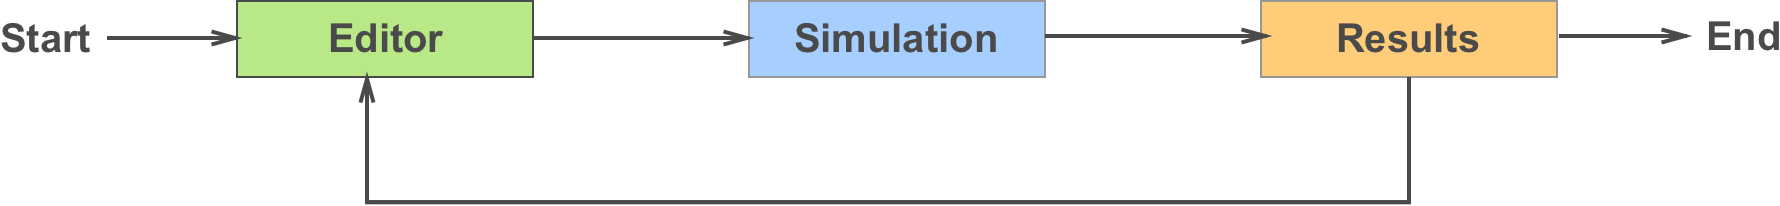
\includegraphics[width=0.9\textwidth]{includes/images/enchainementvue}
 \caption{\label{fig:echainement_vue}Enchaînement des vues dans notre IHM}
\end{figure}
Ce schéma montre l'enchaînement des vues de notre application. La classe Main se contente d'ouvrir la vue de l'éditeur et passe le relai à son contrôleur. Lorsqu'une simulation est démarrée, on passe à la vue de la simulation. Une fois la simulation terminée ou stoppée, on passe à la vue du classement final depuis laquelle on peut recommencer une nouvelle simulation en rouvrant l'éditeur ou fermer l'application.
\begin{figure}[H]
 \centering
 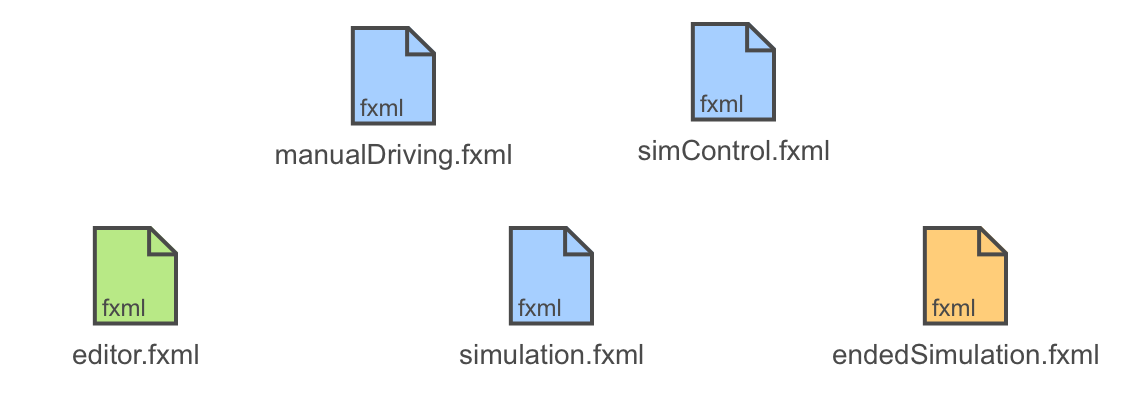
\includegraphics[width=0.7\textwidth]{includes/images/fichiersfxml}
 \caption{\label{fig:fichierfxml}Eléments de notre IHM}
\end{figure}
Nous avons créé un fichier fxml par vue. Pour la simulation, nous avons deux composants fxml supplémentaires qui seront chargés dans la vue en fonction du type de partie. Chaque fichier fxml est rattaché à un contrôleur Java. 
\subsubsection{Éditeur de partie}
\begin{figure}[H]
 \centering
 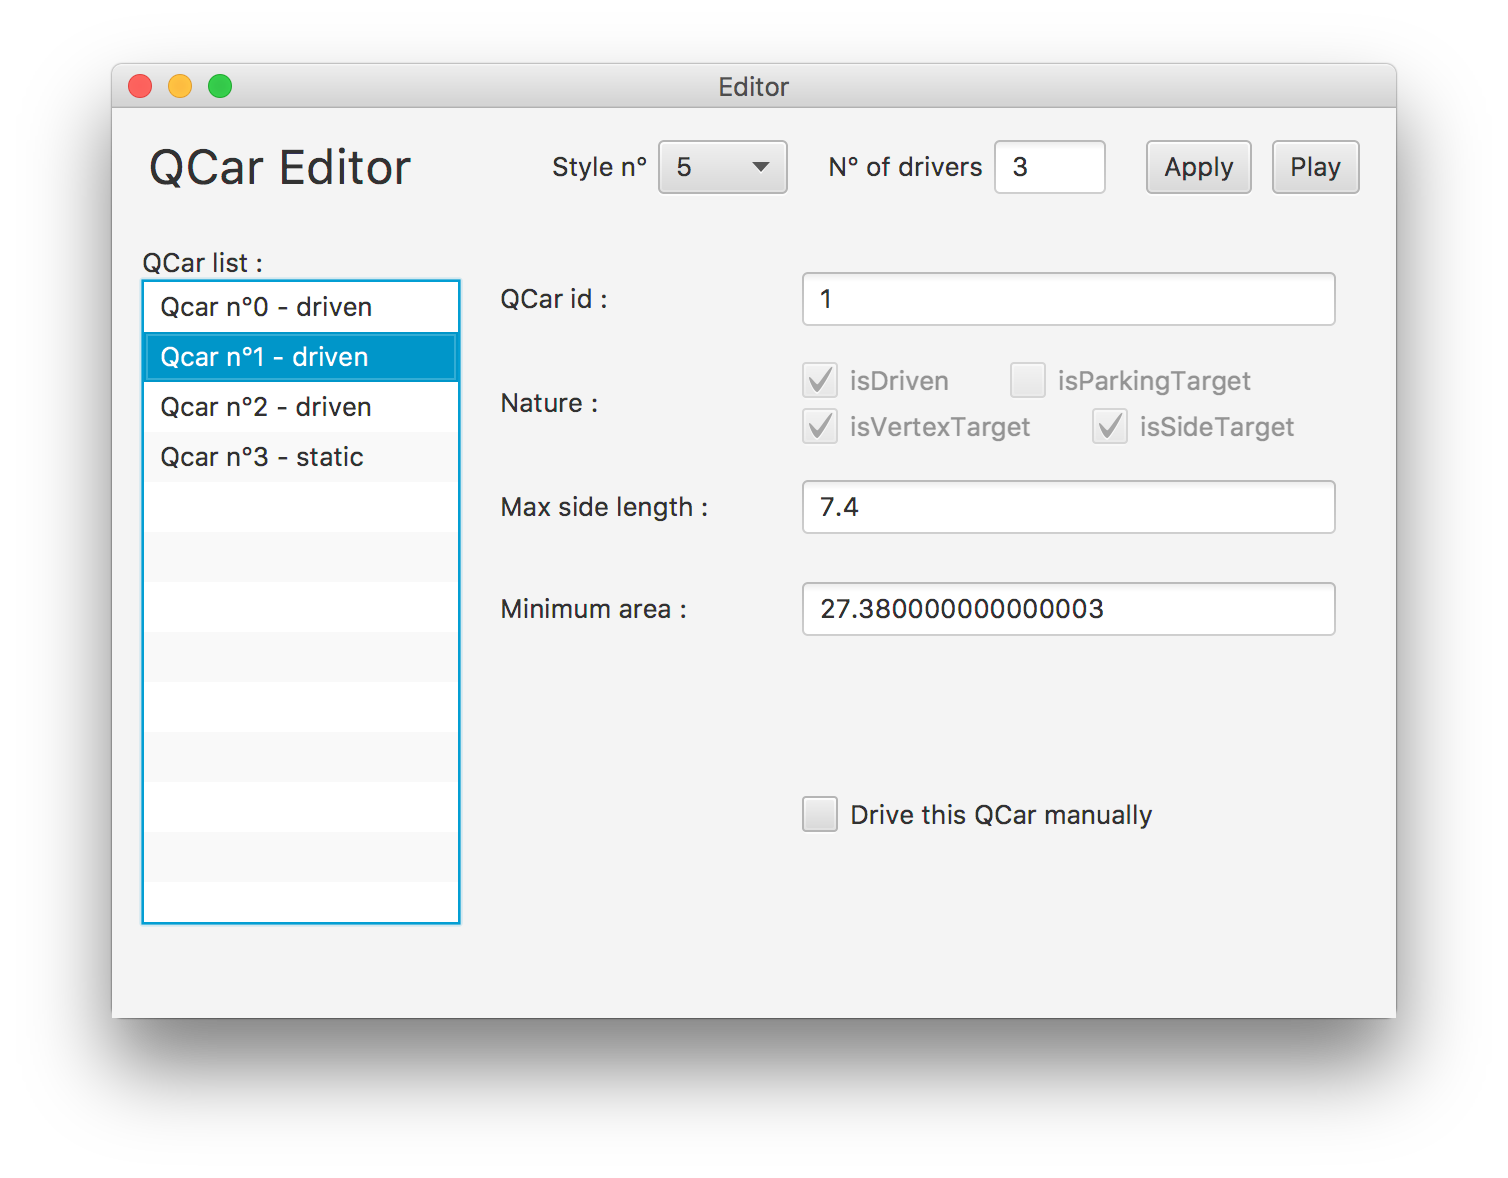
\includegraphics[width=0.9\textwidth]{includes/images/editor}
 \caption{\label{fig:editeur}Éditeur de partie}
\end{figure}
L'éditeur est la vue initiale de l'application. Notre implémentation est très proche de la maquette réalisée durant la phase de conception. L'utilisateur peut choisir un style dans la DropDownList ainsi que le nombre de QCar piloté. Si l'utilisateur rentre une valeur non valide pour le nombre de QCar piloté, un pop up signalera à l'utilisateur qu'il doit entrer un nombre valide. L'utilisateur doit cliquer sur le bouton "Apply" pour générer les QCars. Une fois générés, les QCars apparaissent dans la liste et l'utilisateur peut cliquer sur un QCar afin d'afficher plus d'information à propos de ce QCar. L'utilisateur peut sélectionner un QCar afin de le piloter manuellement, mais il ne peut pas modifier la nature du QCar. Le bouton "Play" n'est cliquable que lorsqu'une liste de QCar est générée. Lorsque le bouton "Play" est cliqué, le contrôleur va charger la vue de la simulation et récupérer son contrôleur. Il va ensuite instancier un WorldManager à partir de la Factory, générer le nombre de pilotes voulus toujours à partir de la factory, démarrer une nouvelle simulation dans le world manager, il va passer le stage et le world manager aux contrôleurs de la simulation et finalement il va afficher la vue de la simulation dans le stage.
\subsubsection{Simulation}
\begin{figure}[H]
 \centering
 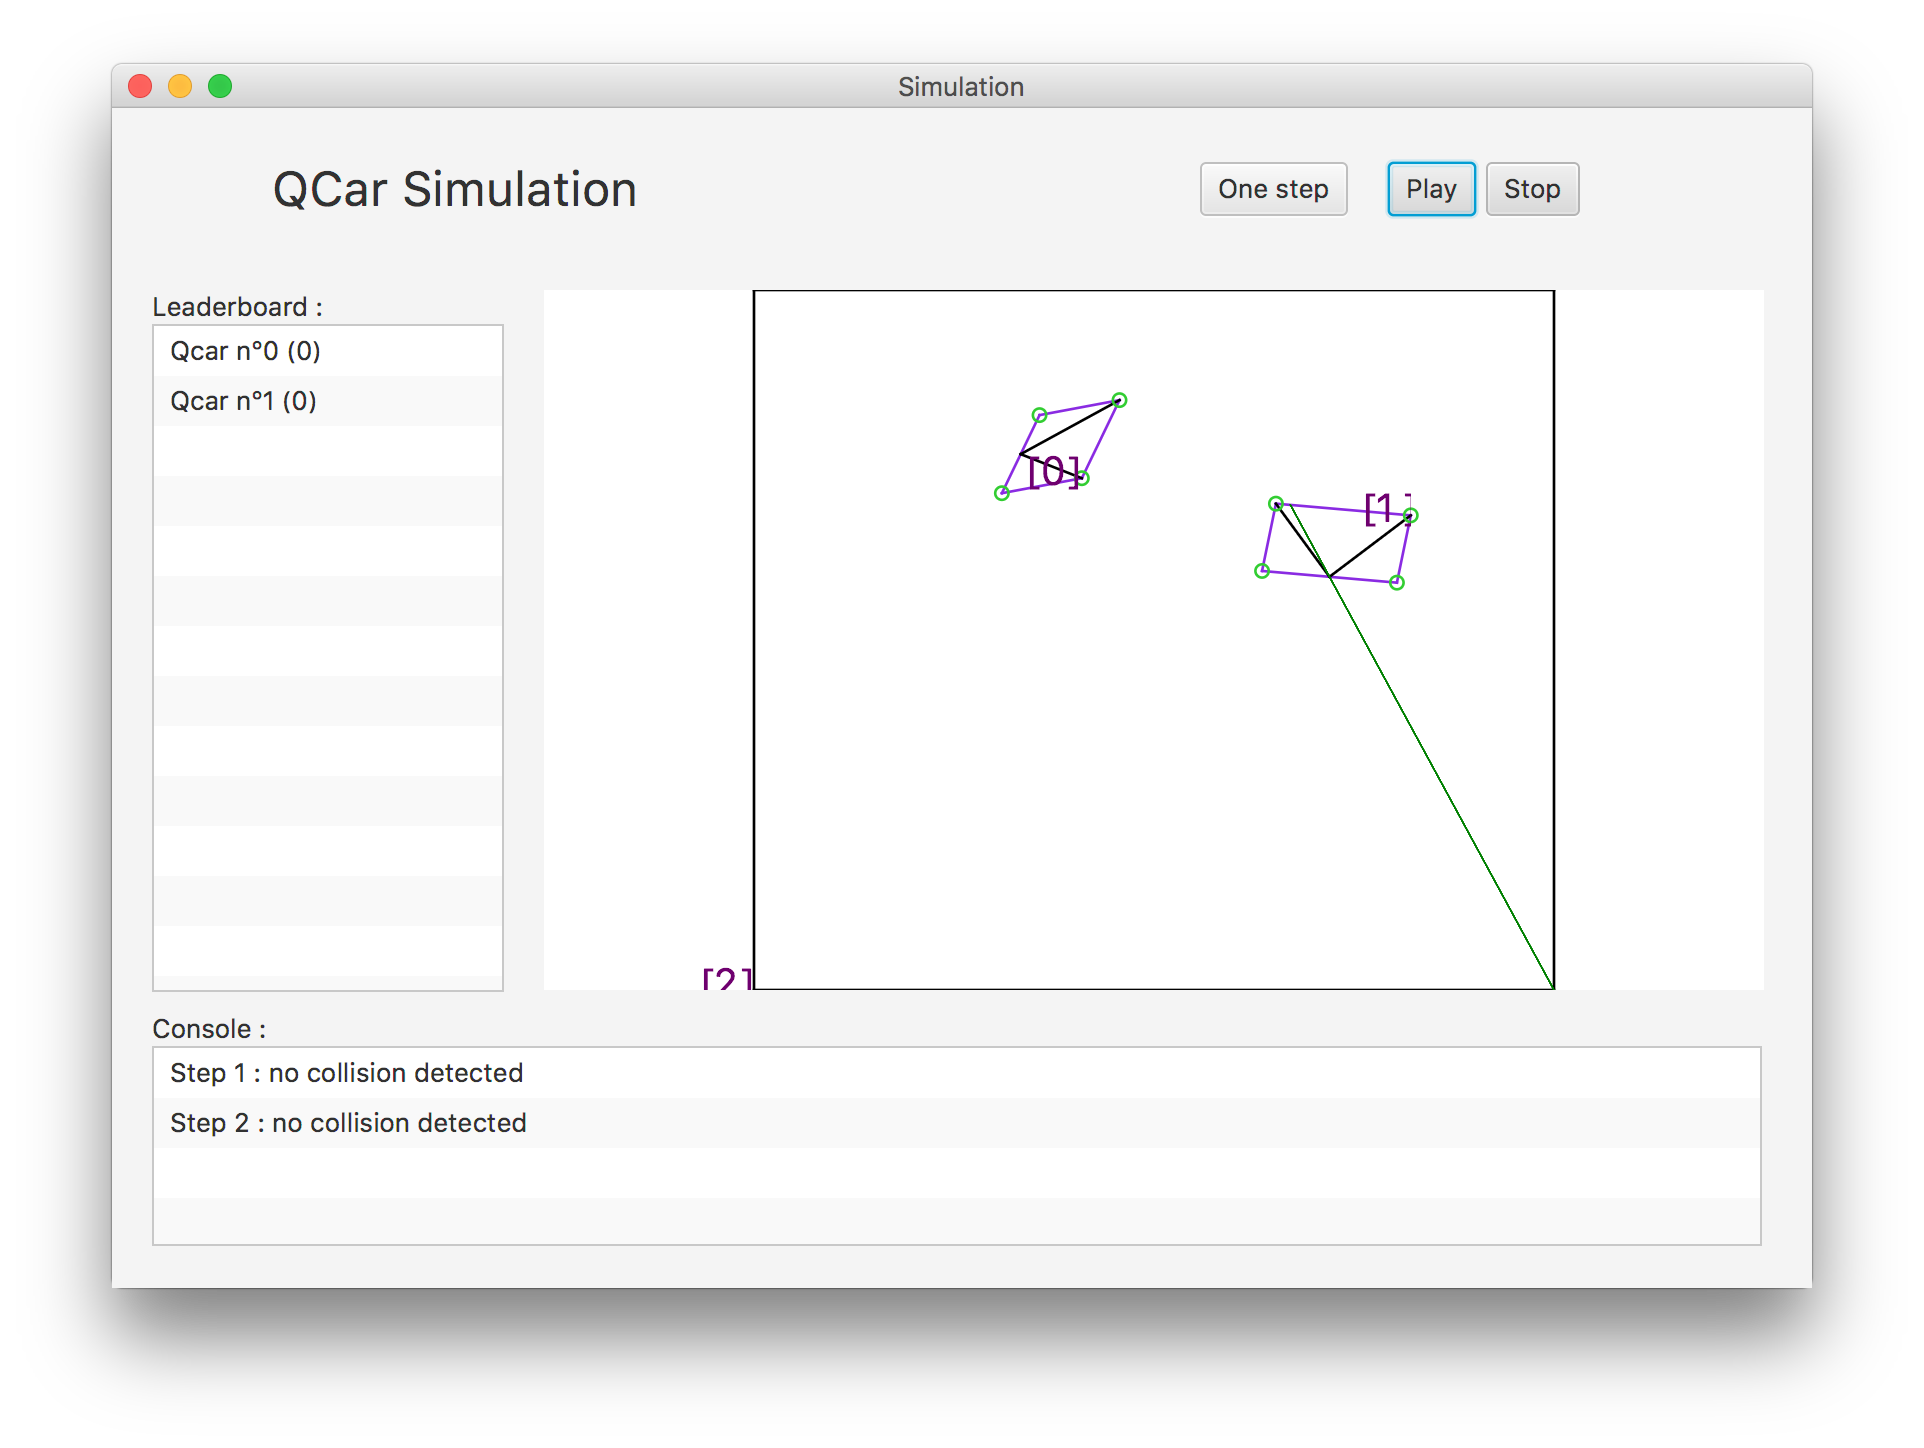
\includegraphics[width=0.7\textwidth]{includes/images/simulation}
 \caption{\label{fig:simulation}Simulation sans QCar piloté manuellement}
\end{figure}
Pour la simulation, nous avons opéré quelques changements par rapport à ce qui était prévu lors de la conception. Nous avons maintenant deux en-têtes: un permettant le contrôle manuel d'un QCar et l'autre servant à gérer la simulation. Le contrôleur de la simulation va charger l'un ou l'autre en-tête en fonction des paramètres qu'il reçoit de l'éditeur. Le reste des éléments est très proche de ce qui était prévu initialement. Nous avons notre classement des QCars pilotés qui est trié en fonction des scores, un panneau permettant de logger les événements de la partie après chaque pas de la simulation et la zone de jeu de nos QCars.
Pour simuler des pas, nous utilisons un service déclaré dans la classe SimControlCtrl. Ce service va appeler la méthode simulateOneStep du WorldManager une fois si l'événement provient du bouton "One Step" ou en boucle si le ToggleButton "Play" est sélectionné. Ce service permet d'isoler le simulateOneStep dans un thread séparé. De cette façon, l'interface graphique ne freeze pas pendant la simulation du pas.
\begin{figure}[H]
 \centering
 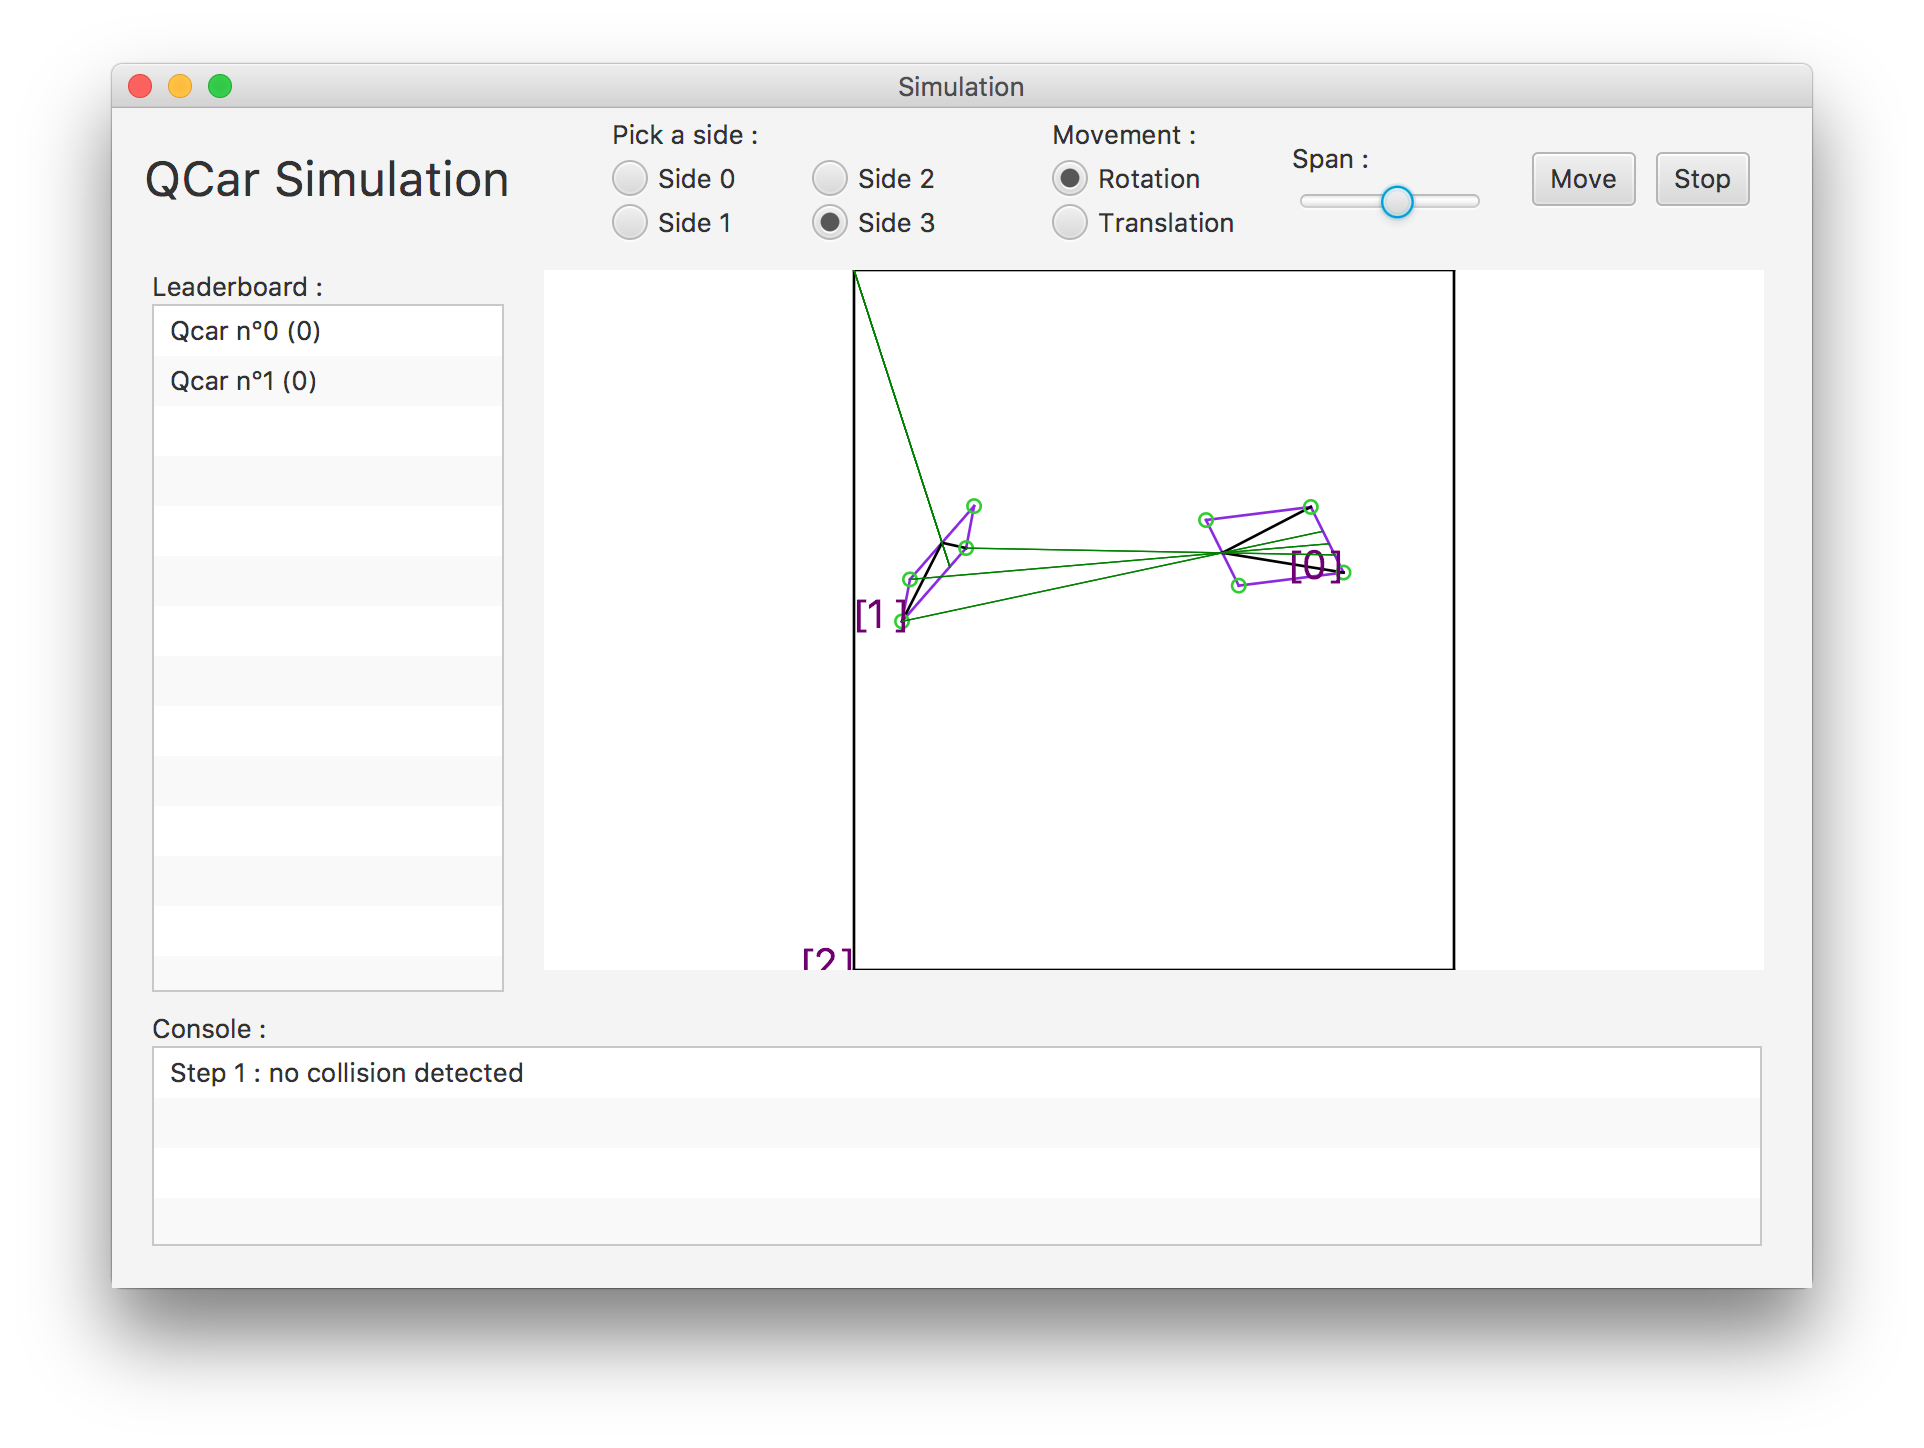
\includegraphics[width=0.7\textwidth]{includes/images/manuelsim}
 \caption{\label{fig:simmanuel}Simulation avec un QCar piloté manuellement}
\end{figure}
Lorsqu'un QCar est sélectionné pour être piloté manuellement, la vue de la simulation chargera l'en-tête ManualDriving ainsi que son contrôleur. Dans cet en-tête, on retrouve tous les paramètres permettant de générer une décision. Le slider permettant de choisir l'envergure d'un mouvement a ses limites redéfinies à chaque fois que le côté ou le type de mouvement sélectionné change. Pour passer la décision manuelle de la vue au world manager, nous avons créer une classe ManualDriver qui implémente l'interface IDriver. De cette façon, le world manager voit le pilote manuel comme un driver normal. Nous utilisons aussi un service pour l'appel de la méthode simulateOneStep(), sauf qu'avant on crée et passe la décision au channel manualDriver.
Malheureusement notre implémentation souffre d'un bug: suivant la position du QCar, les méthodes servant à définir l'envergure minimale et maximale du mouvement retournent des valeurs non valides. À cause de ça, dans certaines configurations le slider n'est pas utilisable rendant certains mouvements impossibles.
Nous avons abandonné l'idée d'implémenter la prévisualisation du mouvement d'un QCar piloté manuellement pour des raisons de temps.
\begin{figure}[H]
 \centering
 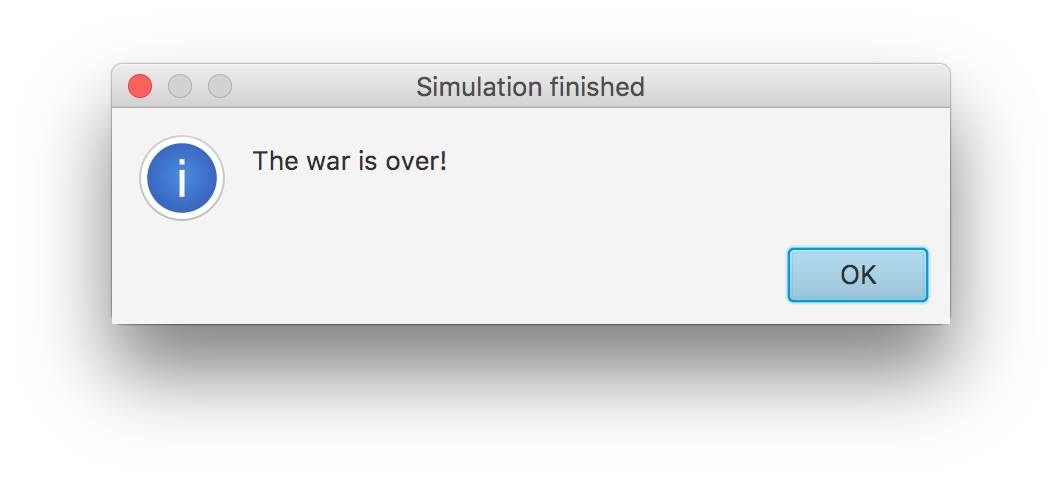
\includegraphics[width=0.7\textwidth]{includes/images/endpopup}
 \caption{\label{fig:endsim}Pop up affiché lorsque la simulation est terminée}
\end{figure}
Afin de détecter la fin de la simulation, la méthode isSimulationOver() est appelée après chaque pas et va appeler la méthode isWarOver() du world manager. Si elle reçoit vrai, un pop up va s'afficher pour prévenir l'utilisateur que la simulation est terminée et lorsque l'utilisateur pressera bouton "Ok", la méthode endSimulation() sera appelée. Cette dernière va fermer la simulation, charger la prochaine vue et lui passer le classement final de la simulation.
Cependant nous avons découvert un bug dans notre implémentation, lorsque le service essaie de créer une Alert lorsque la simulation est terminée, le service reste bloqué dans l'instanciation de l'Alert. Pour remédier à ça, il faut appeler la méthode isSimulationOver non pas depuis le service, mais directement depuis le thread de la vue. 
\subsubsection{Interaction avec la librairie SimViou}
Afin de gérer les interactions entre simviou et notre application, nous avons utilisé une classe UIOp qui implémente UIOperations. Dans cette dernière nous avons défini un méthode qui change le mode de simulation entre STEP\_BY\_STEP et ANIMATION\_RUNNING. Cette méthode est appelée lorsqu'on clique sur le ToggleButton "Play" ou sur le bouton "One Step" dans la simulation. Nous avons aussi ajouté une méthode qui permet de couper ou d'activer le son dans la simulation. Cette méthode est appelée par un raccourci clavier sur la touche "M".
\begin{figure}[H]
 \centering
 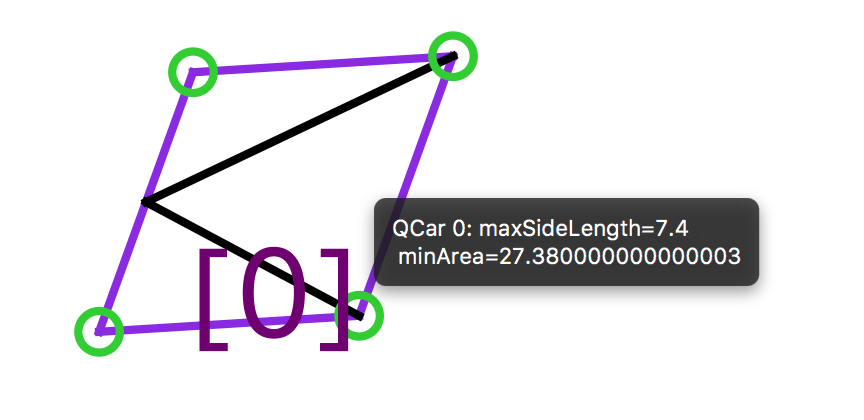
\includegraphics[width=0.7\textwidth]{includes/images/tooltip}
 \caption{\label{fig:tooltip}Tooltip affiché lorsqu'on clique sur un QCar}
\end{figure}
Nous avons ajouté un tooltip lorsqu'on clique sur un QCar dans la simulation. Ce tooltip affiche l'id du QCar sur lequel on a cliqué ainsi que son maxSideLength et son minArea. Nous avons jugé utile d'ajouter ces informations dans un tooltip, car elles ne sont autrement pas visibles pour l'utilisateur depuis la simulation. Afin de détecter si le point où l'utilisateur a cliqué est à l'intérieur d'un QCar, nous utilisons un algorithme nommé PNPOLY.
\subsubsection{Panneau de score}
\begin{figure}[H]
 \centering
 \includegraphics[width=0.7\textwidth]{includes/images/endscreen}
 \caption{\label{fig:scoreboard}Résultats de la simulation}
\end{figure}
La vue finale de notre application, à partir de cette dernière on peut soit fermer l'application soit recommencer une nouvelle simulation à partir de l'éditeur. Le contrôleur de la simulation lui passe le classement final de QCars piloté à la fin de la simulation. Comme pour les autres vues, elle est liée à son propre contrôleur.
Cependant nous avons un bug mineur avec le tri du classement, les QCars sont classés dans l'ordre croissant de leur score. Pour régler ce problème, il faudra modifier l'expression lambda responsable du tri dans la classe SimulationCtrl pour rendre le classement décroissant.
\section{Tests, résultats, améliorations et problèmes}
\subsection{Missing Features}
\subsubsection{Gestion des scores}
Dans la version finale de notre projet, il n'y a aucune gestion des scores. Lors des collisions, il n'y a pas d'échange de points. Le QCar touché ne perd pas de points et le QCar qui touche n'en récupère pas non plus. LE fait de se trouver complètement à l'intérieur d'un parking n'est pas détecté non plus. Cela aurait dû être fait dans le WorldManager, après de la détection des collisions. Les scores des QCars devraient alors être adaptés et les QCars cibles n'apportant plus de points seraient supprimés.
\subsubsection{Utilisation du DistanceSensor par le Driver}
Dans l'"intelligence" du Driver, il n'y a aucune utilisation de la distance par rapport aux autres QCar. Le Driver va tenter de poursuivre la cible qui a le plus de points même si elle est très éloignée alors qu'il y aurait une cible avec légèrement moins de points, mais plus près.
\subsection{Affichage du DistanceSensor} Dans l'IHM, les DistanceSensors ne sont pas affichés.
\subsection{Raccourcis clavier} Il aurait été souhaitable d'implémenter plus de raccourcis clavier pour rendre le programme plus ergonomique. 
\subsection{Tests}
Notre programme ne passait pas certains tests, autant ceux fournis par les autres groupes que les nôtres. Il n'y a pas grand-chose de plus à dire, car la qualité générale des tests était très faible. Cela s'explique, car nous n'avons jamais exercé cela. C'est un gros point à améliorer. Nous avons tout de même codé des tests pour le WorldManagerPhysicsHelper, notamment pour l'inversion des matrices et les changements de base. Le programme passait ces tests, mais nous n’avons dû recoder les méthodes et pas mis à jour les tests.
\subsection{Améliorations}
\subsubsection{Algorithme de collisions, nombre proche de 0}           
Les collisions sont généralement détectées, mais le déplacement ne s'applique pas en conséquence dû à des erreurs d'arrondies.\\
Solution $\rightarrow$ utilisation de l'objet BigDecimal.\\
Cette solution devrait aussi être utilisée dans le "filtre" des décisions. Dans les cas extrêmes où on a des valeurs proches de 0, dû à un calcul de cos(arcsin()), on se retrouve avec des NaN qui faussent totalement les résultats.
\subsubsection{Algorithme des senseurs}  
Certains vertex sont visibles même derrière d'autres QCar. Du coup la condition des parkings n'a pas été implémentée. On peut   actuellement voir à travers un parking, car tous les vertices dans la zone visible sont vus et non parce que sa nature est un parking.
Dans le calcul du senseur de distance, on ne vérifie pas la nature du  QCar que l'on intersecte. Si c'est un parking, le DistanceSensor devrait voir au travers et sinon non.\\
Solution $\rightarrow$ introduction de tests conditionnels (if).
\subsection{Problèmes rencontrés}
Cette section présente des problèmes rencontrés pendant la réalisation du projet qui n'ont pas été présentées dans les autres sections du rapport, car ils n'étaient pas directement en relation avec les autres chapitres.
\subsubsection{Blocage du JavaFX Thread}
Pendant la phase d'implémentation, un problème est survenu lorsqu'il a fallu connecter les différents composants du projet pour la première fois. Ce problème se produisait lorsque le bouton "One Step" était pressé dans l'interface graphique. Une fois le bouton cliqué, la fenêtre devenait grisée et le programme ne répondait plus au point où le système d'exploitation proposait de le quitter vu qu'il ne répondait plus.
\paragraph{Analyse du problème}
Ce clic était intercepté par le Thread en charge de la gestion de cette même interface, nommé JavaFX Thread. En théorie, ce Thread ne doit pas être utilsé pour réaliser des traitements longs ou bloquants, car il est constitué d'une boucle infinie responsable de la réactivité de la fenêtre. Si ce Thread se bloque, la fenêtre se gèle et le système d'exploitation considère l'application comme plantée. 
\paragraph{Cause du problème}
Plusieurs lancements du programme avec le débogueur ont été nécessaires pour trouver la cause du problème. Finalement, la cause a été identifiée. Ce problème était engendré par le fait que le JavaFX Thread tentait de s'appeler lui-même, mais n'était pas disponible pour répondre à sa propre demande. C'est précisément à la ligne 71 de la classe AnimationPane fournie par la librairie SimViou que cet appel a lieu:
\begin{lstlisting}[language=Java]
71  UITools.runFX(() -> { worldStateChanged(); },
72  blockingWorldListener);
\end{lstlisting}
\paragraph{Solution du problème}
Dans un premier temps, ce problème a été contourné en créant un nouveau Thread dans le handler en charge de réagir au clic sur le bouton "One Step". Cette solution a fonctionné et a permis d'établir avec certitude qu'il s'agissait bien d'un deadlock du JavaFX Thread. L'implémentation finale utilise un Service et est décrite plus en détail dans la section correspondant à l'implémentation de l'IHM. Ce problème ne se serait probablement pas produit si la constante booléenne IS\_WORLD\_LISTENER\_BLOCKING déclaré à la ligne 17 de la classe QCarAnimationPane fournie par la librairie qcar-ui était initialisé à false.
\section{Critique, analyse des modules imposés}
Gui 1, WorldManager F, GameProvider E, Driver A
\subsection{Conformité par rapport à la spécification}
Le WorldManager F est correct du point de vue de la détection des SeenVertices et des DistanceSensors. Les collisions sont généralement bien gérées, mais avec parfois des "collisions fantômes" détectées alors qu'il n'y en a pas. Ce cas se produisait souvent avec le vertex 0 du QCar 0. Les QCars n'offrant plus de points sont correctement effacés. 
\subsection{Performances}
La plupart des simulations effectuées se terminaient par un "ABORT" après 1000 pas de simulation.
\subsection{Capacité du pilote}
Le QCar dirigé tourne souvent sur lui-même alors qu'il voit des sommets avec des points. Il se bloque parfois sans raison. Il tente de forcer le passage contre un obstacle et répète les mêmes décisions sans remarquer le blocage. Dans certaines configurations il arrive tout de même à marquer quelques points.
\subsection{Pertinence des configurations de jeu}
Le GameProvider E ne génère qu'une seule configuration de jeu : 5 QCar, dont 1 est conduit et les 4 autres sont fixes. Il n'y a pas de parking.
\subsection{Robustesse}
Parfois le WorldManager F ne respecte parfois pas les contraintes de taille (maxSideLength et minArea de la QCarNature). Avec le Driver B, le World Manager F n'empêche pas le QCar de sortir de la Bounding Box. 
\subsection{Critique de l'IHM gui1}
\paragraph{Configuration de la simulation}
Les éléments nécessaires au lancement d'une partie sont bien présents. Le fait d'avoir la configuration de la partie dans une seconde fenêtre placée devant celle de la simulation peut poser problème. En effet, si l'ulisateur clique sur la fenêtre de la simulation, la fenêtre de configuration de la partie passe en arrière-plan et n'est plus visible. De plus les boutons présents dans la fenêtre de simulation sont cliquables même s’il n'y pas de simulation en cours. Des exceptions sont levées dans la console si on clique sur de ces boutons. Nous avons trouvé un bug où la simulation est lancée avec trois QCars pilotés, et ce même si on configure la partie pour avoir plus ou moins de trois pilotes. Afin de reproduire le bug, il faut simplement insérer une valeur dans le Spinner "Number of drivers" manuellement (sans utiliser les boutons sur le côté).
\paragraph{Simulation sans pilote manuel}
La simulation en mode automatique est très fluide. On perd le zoom lorsqu'on simule un pas et il n'est pas possible de zoomer pendant que la simulation est en mode automatique. À part ça, le reste des éléments semble bien fonctionner.
\paragraph{Simulation avec pilote manuel}
Lorsqu'on souhaite faire un déplacement manuel avec l'interface graphique, on ne peut pas faire de mouvement d'angle. De plus, l'application lève des exceptions dans la console lorsqu'on augmente ou décrémente l'envergure du déplacement. La fenêtre de prévisualisation du mouvement est une très bonne idée et fonctionne bien. Les raccourcis clavier permettant de déplacer le QCar s'appliquent bien dans la fenêtre de prévisualisation cependant nous n'avons pas trouver comment appliquer le déplacement dans la simulation.
\paragraph{Conclusion}
Nous avons trouvé que cette interface est bien pensée. L'utisation des keybinds pour bouger un QCar est une très bonne idée. Le fait d'avoir une petite fenêtre contenant une prévisualisation est aussi une bonne idée. Outre les quelques bugs que nous avons trouvés, nous jugeons cette interface plutôt bonne.
\section{Contributions personnelles au projet}
\newcommand*\rot{\rotatebox{90}} %rotate the table headers
\newcommand*\me{\textbullet} %bullet for the table attributions
\subsection{Projet en général}
\label{tabletaches}
\begin{table}[H]
 \centering
 \begin{tabular}[]{l|c|c|c|c|c|}
   Tâche           & \rot{Cédric Bouteille} & \rot{Jérôme Vonlanthen} & \rot{Karim Romanens} & \rot{Natanael Braga} & \rot{Nicolas Fuchs} \\\hline      
   PVs des réunions    & \me  &\me      & \me     & \me              &\me              \\\hline
   Gestion Git        & ~     &~      & ~              & \me              &~              \\\hline
   Planning          & ~                & ~                & \me              & ~              & ~              \\\hline
   GameProvider               & \me                & ~                 & ~              & \me              & ~              \\\hline
   Physique et collisions              & ~                & ~                 & ~              & \me              & \me              \\\hline
   WorldManager              & \me                & \me                 & \me             & \me              & \me
   \\\hline
   PlayerChannel               & ~                & ~                 & \me              & ~              & ~ \\\hline
   Decision              & ~                & \me                & ~              & ~              & ~ \\\hline
   Driver              & ~                & \me                & ~              & ~              & ~\\\hline
   IHM              & ~                & ~                & \me       &         ~          & \me  \\\hline
 \end{tabular}
\end{table}
\subsection{Rapport du projet}
\begin{table}[H]
 \centering
 \begin{tabular}{l|c|c|c|c|c|}
  Tâche           & \rot{Cédric Bouteille} & \rot{Jérôme Vonlanthen} & \rot{Karim Romanens} & \rot{Natanael Braga} & \rot{Nicolas Fuchs} \\\hline 
  Logo & ~              & ~               & ~            & ~            & \me               \\\hline
  Introduction & ~              & \me               & ~            & ~            & ~               \\\hline
  
  Organisation du projet    & ~   &  ~    & \me       & ~       & ~       \\\hline
  Analyse               & ~          & ~       & \me      & \me    & ~    \\\hline
  GameProvider               & \me                & ~                 & ~              & ~              & ~              \\\hline
  Physique et collisions              & ~                & ~                 & ~              & \me              & \me              \\\hline
  WorldManager              & ~                & \me                 & ~              & ~              & \me
  \\\hline
  PlayerChannel               & ~                & ~                 & \me              & ~              & ~ \\\hline
  Decision              & ~                & \me                & ~              & ~              & ~ \\\hline
  Driver              & ~                & \me                & ~              & ~              & ~\\\hline
  IHM              & ~                & ~                & \me       &         ~          & ~  \\\hline
 \end{tabular}
\end{table}
\section{Conclusion}
Malgré le fait que nous n'ayons pas réussi à implémenter notre application comme nous l'aurions souhaité, ce projet a été une expérience intéressante. Nous nous rejoignons dans l'idée qu'il aurait fallut qu'un des membres assume de manière tacite ou non la gestion du groupe pendant les huit premières semaines et force quelque peu les autres membres à prendre leurs responsabilités quant aux décisions qui étaient prises chaque semaine. Nous pensons qu'il aurait été pertinent d'assigner les rôles de gestion de projet classiques dès la première semaine.\\
L'entente au sein du groupe a bien fonctionné, cependant un manque d'initiative et de communication s'est fait sentir au début du projet. Il est intéressant de noter qu'après la phase des tests d'API, presque tous les membres du groupe ont redirigé leur choix initial vers un autre composant du projet de manière naturelle, permettant ainsi à chacun de se diriger vers un composant qui s'adaptait mieux à ses compétences. Nous sommes restés majoritairement solidaires dans les périodes proches des échéances. Un des objectifs majeurs dans un projet impliquant autant de membres à ce moment de notre formation est de découvrir les "joies" du travail en équipe. Pour parvenir à cette fin, nous avons tenté de mettre en place des outils qui auraient du nous aider à réussir tels que notre scrum en ligne. Au final, nous avons laissé Trello un peu de côté ce qui ne nous a pas empêché d'acquérir une certaine compétence dans l'art de l'organisation.

\subsection{Conclusions individuelles}
\subsubsection{Cédric Bouteille}
Ce projet aura été pour moi un vrai test sur mes capacités de gestion d'imprévus, notamment en ayant eu ma machine hors service pendant une semaine, ce qui a provoqué un effet de cascade m'empêchant de progresser à la fois dans le projet et dans les cours. Cette accumulation de retards m'aura confronté à mes propres limites et a eu l'effet d'une grosse piqure de rappel sur l'importance de la gestion de projet et des priorités.\\
Concernant les tests et l'apprentissage de la rédaction de ceux-ci, je rejoins l'avis Jérôme Vonlanthen sur le sujet.\\
J'ai aussi pu constater que lors d'un projet de plusieurs semaines, on peut vite tomber de manière inconsciente dans le phénomène de report des tâches à plus tard et qu'il est important d'avoir des réunions hebdomadaires pour faire le point sur l'avancement et pouvoir réagir au plus vite en cas de problèmes.
\subsubsection{Jérôme Vonlanthen}
Tout en étant conscient que le but principal de ce projet était de mettre l'accent sur l'organisation au sein du groupe et de nous laisser nous débrouiller, j'aurais apprécié d'être un peu plus guidé. Par exemple une suggestion dans l'ordre ou la priorité des composants à développer ou alors augmenter le nombre de "points" de contrôles, de rendu de petites parties de code, avec un retour sur les choses à améliorer. Une autre amélioration pourrait venir du point de vue des tests. Il serait bénéfique d'apprendre à rédiger de "bons" tests ce qui nous permettrait d'être plus efficaces pour la suite du projet.\\ 
Malgré ces points, ce projet a, pour moi, permis de nous confronter à une situation de travail de groupe. On remarque très vite les différents caractères des membres de l'équipe et il faut réussir à les concilier pour travailler ensemble. Il est également nécessaire que quelqu'un prenne le "lead" et soit la personne qui anime les discussions. C'est cette partie qui, à mon avis, nous a manqué pendant ce projet. La gestion du projet ainsi que la planification sont également des éléments très importants que nous n'avons pas assez considérés.\\
En voyant le résultat de la plupart des groupes lors de la mise en commun des composants, il n'y a pas vraiment de programmes fonctionnels et c'est dommage. D'où mes remarques sur un suivi un peu plus marqué.
\subsubsection{Karim Romanens}
J'aurais apprécié être un peu plus accompagné tout au long du projet. Par exemple, placer quelques checkpoints durant le travail où certaines fonctionnalités doivent être implémentées et rendues. Cela nous aurait permis d'avoir des feedbacks réguliers et nous aurait aidés à mieux choisir quelles tâches priorisées.\\ J'ai trouvé qu'en général les documents fournis manquaient de clarté cependant les professeurs étaient toujours présents pour répondre aux éventuelles questions et éclaircir certains points. \\ Ce projet m'a permis de me rendre compte que mener un projet entier à bien n'est pas une mince affaire. J'ai trouvé très difficile de commencer le projet, car plein d'éléments dépendent les uns des autres et c'était compliqué de choisir par où commencer. \\ Je suis quand même un peu déçu du résultat final de notre projet. Avec une meilleure gestion de notre temps, je pense qu'on aurait pu avoir un projet bien plus fonctionnel.\\ L'entente au sein de notre groupe était globalement bonne. Pour les prochains projets, il faudra vraiment que je remplisse mon journal de travail au fur et à mesure, car il n'est parfois pas évident de se rappeler des tâches que l'on a faites la semaine précédente.
\subsubsection{Natanael Braga}
Bien qu'à prime abord le projet QCar paraisse peu intéressant, j'ai apprécié pouvoir travailler à sa réalisation au sein du groupe 4. Il est vrai que notre implémentation n'est pas parfaite et que bon nombre de bugs sont toujours présents. Mais je suis cependant très satisfait du fait que nous ayons réalisé beaucoup d'effort dans la conception de notre implémentation, plutôt que de suivre une approche plus traditionnelle de partir directement dans le code. Nous avons essayé de relever certains défis en utilisant des outils que nous avons acquis pendant notre cursus dans cette école. Ce "pari" quelque peu risqué nous a causé des difficultés vers la fin du projet et a entravé notre capacité à rendre le projet dans l'état où nous l'aurions souhaité. Cependant, cet effort réalisé me donne, personnellement, un sentiment d'accomplissement personnel.\\
De mon point de vue, notre gestion de groupe n'était pas parfaite. Notamment, il était parfois difficile de mettre en route la communication. Une fois que la communication s'établissait, les choses progressaient assez bien. Je résumerais cet aspect en disant qu'à mon avis, il nous manquait un peut une dynamique que d'autres groupes avaient car nous nous connaissions moins au départ.\\
J'ai particulièrement apprécié pouvoir travailler régulièrement en binôme avec différents membres du groupe sur des aspects du code distincts et mettre en place une ambiance d'entraide entre tous. Tous les membres ont founit des efforts et personne ne s'est reposé sur les autres.\\
En conclusion, j'aimerais retenir pour mes futurs projets en groupe l'importance de déléguer les tâches basiques de la gestion de projet dès le début. Ceci pour éviter que le projet ne stagne trop longtemps au départ. Je remercie mes colègues pour le travail réalisé et les superviseurs pour l'aide qu'ils nous ont fourni au long du projet.

\subsubsection{Nicolas Fuchs}
 
J'ai trouvé le concept du jeu très intéressant pour un projet. Par contre je n'ai pas trouvé le jeu en lui-même intéressant. Il fallait bien sûr qu'on travaille sur un projet qui soit réalisable sur un semestre, mais le temps de développement ne valait pas la peine pour ce jeu-là. Surtout que le jeu doit se lancer en ligne de commande sans interface graphique. Je pense que ça aurait été plus motivant si à la base tous les Qcars dirigés devaient être conduits manuellement et ensuite se pencher si on a le temps sur le développement de drivers. Mais que dans tous les cas on se base sur un mode visuel puisque c'est un jeu.\\
La documentation simviou manquait de clarté. Dans la documentation du projet, certains concepts basiques n'étaient pas assez bien expliqués (signe de déplacement par rapport au côté, utilisation obligatoire d'un pane contenant la QCaranimationPane pour l'affichage). Certaines fonctionnalités de l'animationPane étaient difficilement trouvables et pas mises en avant (QCarAnimationPane.COLLISION\_EVENT, …). \\
Le projet était assez difficilement séparable à son début. Tous les modules étaient interdépendants et on ne savait pas trop où partir. De ce côté-là, j'aurais attendu plus de suivis et de suggestions. On ne pouvait pas bien prédire qu'est-ce qui prendrait le plus de temps à développer et comment bien répartir les tâches. Certaines ont demandé énormément de temps tandis que d'autres très peu. Dans ce domaine-là, on aurait pu un peu mieux répartir les tâches. \\
La gestion du temps n'était pas évidente non plus. Le temps est très vite passé. \\
J'ai trouvé que le travail était un peu trop individuel certaines fois. Alors bien sûr, on ne peut pas toujours tous être sur le même fichier en même temps. Mais travailler un peu plus en binôme aurait été plus agréable surtout au commencement du projet lorsqu' on ne sait pas trop comment partir. \\
Lors de problèmes par contre, l'entre-aide a été satisfaisante. On s'est toujours mis ensemble pour régler un souci lorsqu'il y en avait un chez un des membres du groupe.\\
L'ambiance de groupe était généralement bonne. Par contre lorsque l'on se donnait rendez-vous, certaines personnes n'étaient pas là, mais travaillaient quand même à la maison. Ça ne renforce pas l'esprit de communication et d'équipe. La communication aurait pu être un peu améliorée.
\label{findudocument}
\section{Annexes}
\begin{itemize}
\item PVs des réunions
\item Journaux de travail
\end{itemize}
\includepdf[pages=-]{includes/pvs/P1-24022017.pdf}
\includepdf[pages=-]{includes/pvs/P2-27022017.pdf}
\includepdf[pages=-]{includes/pvs/P3-06032017.pdf}
\includepdf[pages=-]{includes/pvs/P4-17032017.pdf}
\includepdf[pages=-]{includes/pvs/P5-20032017.pdf}
\includepdf[pages=-]{includes/pvs/P6-27032017.pdf}
\includepdf[pages=-]{includes/pvs/P8-10042017.pdf}
\includepdf[pages=-]{includes/pvs/P9-24042017.pdf}
\includepdf[pages=-]{includes/pvs/P10-03052017.pdf}
\includepdf[pages=-]{includes/pvs/P11-11052017.pdf}
\includepdf[pages=-]{includes/pvs/P12-18052017.pdf}
\includepdf[pages=-]{includes/pvs/P13-22052017.pdf}
\includepdf[pages=-]{includes/pvs/P14-29052017.pdf}
\includepdf[pages=-]{includes/pvs/Bouteille.pdf}
\includepdf[pages=-]{includes/pvs/Vonlanthen.pdf}
\includepdf[pages=-]{includes/pvs/Romanens.pdf}
\includepdf[pages=-]{includes/pvs/Braga.pdf}
\includepdf[pages=-]{includes/pvs/Fuchs.pdf}
\end{document}